% !TeX spellcheck = russian-aot-ieyo
% Зачем: Определяет класс документа (То, как будет выглядеть документ)
% Примечание: параметр draft помечает строки, вышедшие за границы страницы, прямоугольником, в фильной версии его нужно удалить.
\documentclass[a4paper,14pt,russian,oneside,final]{extreport}

% Зачем: Настройка Times New Roman.
% Рекомендовано для Windows (нужен PSCyr, подробности см. в fonts_windows.tex)
% раскомментировать, чтобы использовать:
%\input{fonts_windows}% не забудьте закомментировать \input{fonts_linux}

% Рекомендовано для Linux (нужен scalable-cyrfonts-tex, подробности см. в fonts_linux.tex)
% раскомментировать, чтобы использовать:
\input{fonts_linux}% не забудьте закомментировать \input{fonts_windows}

% Зачем: Установка кодировки исходных файлов.
\usepackage[utf8]{inputenc}

% Зачем: Делает результирующий PDF "searchable and copyable".
\usepackage{cmap}

% Зачем: Чтобы можно было использовать русские буквы в формулах, но в случае использования предупреждать об этом.
\usepackage[warn]{mathtext}

% Зачем: Учет особенностей различных языков.
\usepackage[russian]{babel}

% Зачем: Добавляет поддержу дополнительных размеров текста 8pt, 9pt, 10pt, 11pt, 12pt, 14pt, 17pt, and 20pt.
% Почему: Пункт 2.1.1 Требований по оформлению пояснительной записки.
\usepackage{extsizes}


% Зачем: Длинна, пимерно соответвующая 5 символам
% Почему: Требования содержат странное требование про отсупы в 5 символов (для немоноширинного шрифта :| )
\newlength{\fivecharsapprox}
\setlength{\fivecharsapprox}{6ex}


% Зачем: Добавляет отступы для абзацев.
% Почему: Пункт 2.1.3 Требований по оформлению пояснительной записки.
\usepackage{indentfirst}
\setlength{\parindent}{\fivecharsapprox} % Примерно соответсвует 5 символам.


% Зачем: Настраивает отступы от границ страницы.
% Почему: Пункт 2.1.2 Требований по оформлению пояснительной записки.
\usepackage[left=3cm,top=2.0cm,right=1.5cm,bottom=2.7cm]{geometry}


% Зачем: Настраивает межстрочный интервал, для размещения 40 +/- 3 строки текста на странице.
% Почему: Пункт 2.1.1 Требований по оформлению пояснительной записки.
\usepackage[nodisplayskipstretch]{setspace}
\setstretch{1.1}
%\onehalfspacing

% Зачем: Выбор шрифта по-умолчанию.
% Почему: Пункт 2.1.1 Требований по оформлению пояснительной записки.
% Примечание: В требованиях не указан, какой именно шрифт использовать. По традиции используем TNR.
\renewcommand{\rmdefault}{ftm} % Times New Roman


% Зачем: Отключает использование изменяемых межсловных пробелов.
% Почему: Так не принято делать в текстах на русском языке.
\frenchspacing


% Зачем: Сброс счетчика сносок для каждой страницы
% Примечание: в "Требованиях по оформлению пояснительной записки" не указано, как нужно делать, но в других БГУИРовских докуметах рекомендуется нумерация отдельная для каждой страницы
\usepackage{perpage}
\MakePerPage{footnote}


% Зачем: Добавляет скобку 1) к номеру сноски
% Почему: Пункты 2.9.2 и 2.9.1 Требований по оформлению пояснительной записки.
\makeatletter
\def\@makefnmark{\hbox{\@textsuperscript{\normalfont\@thefnmark)}}}
\makeatother


% Зачем: Расположение сносок внизу страницы
% Почему: Пункт 2.9.2 Требований по оформлению пояснительной записки.
\usepackage[bottom]{footmisc}


% Зачем: Переопределяем стандартную нумерацию, т.к. в отчете будут только section и т.д. в терминологии TeX
\makeatletter
\renewcommand{\thesection}{\arabic{section}}
\makeatother


% Зачем: Пункты (в терминологии требований) в терминологии TeX subsubsection должны нумероваться
% Почему: Пункт 2.2.3 Требований по оформлению пояснительной записки.
\setcounter{secnumdepth}{3}


% Зачем: Настраивает отступ между таблицей с содержанимем и словом СОДЕРЖАНИЕ
% Почему: Пункт 2.2.7 Требований по оформлению пояснительной записки.
\usepackage{tocloft}
\setlength{\cftbeforetoctitleskip}{-1em}
\setlength{\cftaftertoctitleskip}{1em}


% Зачем: Определяет отступы слева для записей в таблице содержания.
% Почему: Пункт 2.2.7 Требований по оформлению пояснительной записки.
\makeatletter
\renewcommand{\l@section}{\@dottedtocline{1}{0.5em}{1.2em}}
\renewcommand{\l@subsection}{\@dottedtocline{2}{1.7em}{2.0em}}
\makeatother


% Зачем: Работа с колонтитулами
\usepackage{fancyhdr} % пакет для установки колонтитулов
\pagestyle{fancy} % смена стиля оформления страниц


% Зачем: Нумерация страниц располагается справа снизу страницы
% Почему: Пункт 2.2.8 Требований по оформлению пояснительной записки.
\fancyhf{} % очистка текущих значений
\fancyfoot[R]{\thepage} % установка верхнего колонтитула
\renewcommand{\footrulewidth}{0pt} % убрать разделительную линию внизу страницы
\renewcommand{\headrulewidth}{0pt} % убрать разделительную линию вверху страницы
\fancypagestyle{plain}{
    \fancyhf{}
    \rfoot{\thepage}}


% Зачем: Задает стиль заголовков раздела жирным шрифтом, прописными буквами, без точки в конце
% Почему: Пункты 2.1.1, 2.2.5, 2.2.6 и ПРИЛОЖЕНИЕ Л Требований по оформлению пояснительной записки.
\makeatletter
\renewcommand\section{%
  \clearpage\@startsection {section}{1}%
    {\fivecharsapprox}%
    {-1em \@plus -1ex \@minus -.2ex}%
    {1em \@plus .2ex}%
    {\raggedright\hyphenpenalty=10000\normalfont\large\bfseries\MakeUppercase}}
\makeatother


% Зачем: Задает стиль заголовков подразделов
% Почему: Пункты 2.1.1, 2.2.5 и ПРИЛОЖЕНИЕ Л Требований по оформлению пояснительной записки.
\makeatletter
\renewcommand\subsection{%
  \@startsection{subsection}{2}%
    {\fivecharsapprox}%
    {-1em \@plus -1ex \@minus -.2ex}%
    {1em \@plus .2ex}%
    {\raggedright\hyphenpenalty=10000\normalfont\normalsize\bfseries}}
\makeatother


% Зачем: Задает стиль заголовков пунктов
% Почему: Пункты 2.1.1, 2.2.5 и ПРИЛОЖЕНИЕ Л Требований по оформлению пояснительной записки.
\makeatletter
\renewcommand\subsubsection{
  \@startsection{subsubsection}{3}%
    {\fivecharsapprox}%
    {-1em \@plus -1ex \@minus -.2ex}%
    {\z@}%
    {\raggedright\hyphenpenalty=10000\normalfont\normalsize\bfseries}}
\makeatother

% Зачем: для оформления введения и заключения, они должны быть выровнены по центру.
% Почему: Пункты 1.1.15 и 1.1.11 Требований по оформлению пояснительной записки.
\makeatletter
\newcommand\sectioncentered{%
  \clearpage\@startsection {section}{1}%
    {\z@}%
    {-1em \@plus -1ex \@minus -.2ex}%
    {1em \@plus .2ex}%
    {\centering\hyphenpenalty=10000\normalfont\large\bfseries\MakeUppercase}%
    }
\makeatother



% Зачем: Задает стиль библиографии
% Почему: Пункт 2.8.6 Требований по оформлению пояснительной записки.
\bibliographystyle{styles/belarus-specific-utf8gost780u}


% Зачем: Пакет для вставки картинок
% Примечание: Объяснение, зачем final - http://tex.stackexchange.com/questions/11004/why-does-the-image-not-appear
\usepackage[final]{graphicx}
\DeclareGraphicsExtensions{.pdf,.png,.jpg,.eps}


% Зачем: Директория в которой будет происходить поиск картинок
\graphicspath{{figures/}}


% Зачем: Добавление подписей к рисункам
\usepackage[nooneline]{caption}
\usepackage{subcaption}

% Зачем: чтобы работала \No в новых латехах
\DeclareRobustCommand{\No}{\ifmmode{\nfss@text{\textnumero}}\else\textnumero\fi}

% Зачем: поворот ячеек таблиц на 90 градусов
\usepackage{rotating}
\DeclareRobustCommand{\povernut}[1]{\begin{sideways}{#1}\end{sideways}}


% Зачем: когда в формулах много кириллических символов команда \text{} занимает много места
\DeclareRobustCommand{\x}[1]{\text{#1}}


% Зачем: Задание подписей, разделителя и нумерации частей рисунков
% Почему: Пункт 2.5.5 Требований по оформлению пояснительной записки.
\DeclareCaptionLabelFormat{stbfigure}{Рисунок #2}
\DeclareCaptionLabelFormat{stbtable}{Таблица #2}
\DeclareCaptionLabelSeparator{stb}{~--~}
\captionsetup{labelsep=stb}
\captionsetup[figure]{labelformat=stbfigure,justification=centering}
\captionsetup[table]{labelformat=stbtable,justification=raggedright}
\renewcommand{\thesubfigure}{\asbuk{subfigure}}

% Зачем: Окружения для оформления формул
% Почему: Пункт 2.4.7 требований по оформлению пояснительной записки и специфические требования различных кафедр
% Пример использования смотри в course_content.tex, строка 5
\usepackage{calc}
\newlength{\lengthWordWhere}
\settowidth{\lengthWordWhere}{где}
\newenvironment{explanationx}
    {%
    %%% Следующие строки определяют специфические требования разных редакций стандартов. Раскоменнтируйте нужную строку
    %% стандартный абзац, СТП-01 2010
    %\begin{itemize}[leftmargin=0cm, itemindent=\parindent + \lengthWordWhere + \labelsep, labelsep=\labelsep]
    %% без отступа, СТП-01 2013
    \begin{itemize}[leftmargin=0cm, itemindent=\lengthWordWhere + \labelsep , labelsep=\labelsep]%
    \renewcommand\labelitemi{}%
    }
    {%
    %\\[\parsep]
    \end{itemize}
    }

% Старое окружение для "где". Сохранено для совместимости
\usepackage{tabularx}

\newenvironment{explanation}
    {
    %%% Следующие строки определяют специфические требования разных редакций стандартов. Раскоменнтируйте нужные 2 строки
    %% стандартный абзац, СТП-01 2010
    %\par
    %\tabularx{\textwidth-\fivecharsapprox}{@{}ll@{ --- } X }
    %% без отступа, СТП-01 2013
    \noindent
    \tabularx{\textwidth}{@{}ll@{ --- } X }
    }
    {
    \\[\parsep]
    \endtabularx
    }


% Зачем: Удобная вёрстка многострочных формул, масштабирующийся текст в формулах, формулы в рамках и др
\usepackage{amsmath}


% Зачем: Поддержка ажурного и готического шрифтов
\usepackage{amsfonts}


% Зачем: amsfonts + несколько сотен дополнительных математических символов
\usepackage{amssymb}


% Зачем: Окружения «теорема», «лемма»
\usepackage{amsthm}


% Зачем: Производить арифметические операции во время компиляции TeX файла
\usepackage{calc}

% Зачем: Производить арифметические операции во время компиляции TeX файла
\usepackage{fp}

% Зачем: Пакет для работы с перечислениями
\usepackage{enumitem}
\makeatletter
 \AddEnumerateCounter{\asbuk}{\@asbuk}{щ)}
\makeatother


% Зачем: Устанавливает символ начала простого перечисления
% Почему: Пункт 2.3.5 Требований по оформлению пояснительной записки.
\setlist{nolistsep}


% % Зачем: Устанавливает символ начала именованного перечисления
% % Почему: Пункт 2.3.8 Требований по оформлению пояснительной записки.
% \renewcommand{\labelenumi}{\asbuk{enumi})}
% \renewcommand{\labelenumii}{\arabic{enumii})}

\renewcommand{\theenumi}{\arabic{enumi}}

\renewcommand{\theenumii}{\arabic{enumii}}

\renewcommand\labelenumi{\theenumi}

\renewcommand\labelenumii{\theenumii}


% Зачем: Устанавливает отступ от границы документа до символа списка, чтобы этот отступ равнялся отступу параграфа
% Почему: Пункт 2.3.5 Требований по оформлению пояснительной записки.

\setlist[itemize,0]{itemindent=\parindent + 2.2ex,leftmargin=0ex,label=--}
\setlist[enumerate,1]{itemindent=\parindent + 2.7ex,leftmargin=0ex}
\setlist[enumerate,2]{itemindent=\parindent + \parindent - 2.7ex}

% Зачем: Включение номера раздела в номер формулы. Нумерация формул внутри раздела.
\AtBeginDocument{\numberwithin{equation}{section}}

% Зачем: Включение номера раздела в номер таблицы. Нумерация таблиц внутри раздела.
\AtBeginDocument{\numberwithin{table}{section}}

% Зачем: Включение номера раздела в номер рисунка. Нумерация рисунков внутри раздела.
\AtBeginDocument{\numberwithin{figure}{section}}


% Зачем: Дополнительные возможности в форматировании таблиц
\usepackage{makecell}
\usepackage{multirow}
\usepackage{array}


% Зачем: "Умная" запятая в математических формулах. В дробных числах не добавляет пробел
% Почему: В требованиях не нашел, но в русском языке для дробных чисел используется {,} а не {.}
\usepackage{icomma}

% Зачем: макрос для печати римских чисел
\makeatletter
\newcommand{\rmnum}[1]{\romannumeral #1}
\newcommand{\Rmnum}[1]{\expandafter\@slowromancap\romannumeral #1@}
\makeatother


% Зачем: Управление выводом чисел.
\usepackage{sistyle}
\SIdecimalsign{,}

% Зачем: inline-коментирование содержимого.
\newcommand{\ignore}[2]{\hspace{0in}#2}


% Зачем: Возможность коментировать большие участки документа
\usepackage{verbatim}


\usepackage{xcolor}


% Зачем: Оформление листингов кода
% Примечание: final нужен для переопределения режима draft, в котором листинги не выводятся в документ.
\usepackage[final]{listings}


% Зачем: настройка оформления листинга для языка F#
\definecolor{bluekeywords}{rgb}{0.13,0.13,1}
\definecolor{greencomments}{rgb}{0,0.5,0}
\definecolor{turqusnumbers}{rgb}{0.17,0.57,0.69}
\definecolor{redstrings}{rgb}{0.5,0,0}

\renewcommand{\lstlistingname}{Листинг}

\lstdefinelanguage{FSharp}
    {morekeywords={abstract,and,as,assert,base,begin,class,default,delegate,do,done,downcast,downto,elif,else,end,exception,extern,false,finally,for,fun,function,global,if,in,inherit,inline,interface,internal,lazy,let,let!,match,member,module,mutable,namespace,new,not,null,of,open,or,override,private,public,rec,return,return!,select,static,struct,then,to,true,try,type,case,upcast,use,use!,val,void,when,while,with,yield,yield!,asr,land,lor,lsl,lsr,lxor,mod,sig,atomic,break,checked,component,const,constraint,constructor,continue,eager,event,external,fixed,functor,include,method,mixin,object,parallel,process,protected,pure,sealed,tailcall,trait,virtual,volatile},
    keywordstyle=\bfseries\color{bluekeywords},
    sensitive=false,
    morecomment=[l][\color{greencomments}]{///},
    morecomment=[l][\color{greencomments}]{//},
    morecomment=[s][\color{greencomments}]{{(*}{*)}},
    morestring=[b]",
    stringstyle=\color{redstrings},
    }

\lstdefinestyle{fsharpstyle}{
   xleftmargin=0ex,
   language=FSharp,
   basicstyle=\footnotesize\ttfamily,
   breaklines=true,
   columns=fullflexible
}

\lstdefinestyle{csharpinlinestyle} {
  language=[Sharp]C,
  morekeywords={yield,var,get,set,from,select,partial,where,async,await},
  breaklines=true,
  columns=fullflexible,
  basicstyle=\footnotesize\ttfamily
}

\lstdefinestyle{json}{
  showstringspaces    = false,
  keywords            = {false,true},
  alsoletter          = 0123456789.,
  morestring          = [s]{"}{"},
  basicstyle=\footnotesize\ttfamily,
  breaklines=true,
  columns=fullflexible
}

\lstdefinestyle{csharpstyle}{
  language=[Sharp]C,
  frame=lr,
  rulecolor=\color{blue!80!black}}


% Зачем: Нумерация листингов в пределах секции
\AtBeginDocument{\numberwithin{lstlisting}{section}}

\usepackage[normalem]{ulem}

\usepackage[final,hidelinks]{hyperref}
% Моноширинный шрифт выглядит визуально больше, чем пропорциональный шрифт, если их размеры одинаковы. Искусственно уменьшаем размер ссылок.
\renewcommand{\UrlFont}{\small\rmfamily\tt}

\usepackage[square,numbers,sort&compress]{natbib}
\setlength{\bibsep}{0em}

% Магия для подсчета разнообразных объектов в документе
\usepackage{lastpage}
\usepackage{totcount}
\regtotcounter{section}

\usepackage{etoolbox}

\newcounter{totfigures}
\newcounter{tottables}
\newcounter{totreferences}
\newcounter{totequation}

\providecommand\totfig{}
\providecommand\tottab{}
\providecommand\totref{}
\providecommand\toteq{}

\makeatletter
\AtEndDocument{%
  \addtocounter{totfigures}{\value{figure}}%
  \addtocounter{tottables}{\value{table}}%
  \addtocounter{totequation}{\value{equation}}
  \immediate\write\@mainaux{%
    \string\gdef\string\totfig{\number\value{totfigures}}%
    \string\gdef\string\tottab{\number\value{tottables}}%
    \string\gdef\string\totref{\number\value{totreferences}}%
    \string\gdef\string\toteq{\number\value{totequation}}%
  }%
}
\makeatother

\pretocmd{\section}{\addtocounter{totfigures}{\value{figure}}\setcounter{figure}{0}}{}{}
\pretocmd{\section}{\addtocounter{tottables}{\value{table}}\setcounter{table}{0}}{}{}
\pretocmd{\section}{\addtocounter{totequation}{\value{equation}}\setcounter{equation}{0}}{}{}
\pretocmd{\bibitem}{\addtocounter{totreferences}{1}}{}{}



% Для оформления таблиц не влязящих на 1 страницу
\usepackage{longtable}

% Для включения pdf документов в результирующий файл
\usepackage{pdfpages}

% Для использования знака градуса и других знаков
% http://ctan.org/pkg/gensymb
\usepackage{gensymb}

% Зачем: преобразовывать текст в верхний регистр командой MakeTextUppercase
\usepackage{textcase}

% Зачем: Переносы в словах с тире.
% Тире в словае заменяем на \hyph: аппаратно\hyphпрограммный.
% https://stackoverflow.com/questions/2193307/how-to-get-latex-to-hyphenate-a-word-that-contains-a-dash#
\def\hyph{-\penalty0\hskip0pt\relax}

% Добавляем абзацный отступ для библиографии
% https://github.com/mstyura/bsuir-diploma-latex/issues/19
\setlength\bibindent{-1.0900cm}

\makeatletter
\renewcommand\NAT@bibsetnum[1]{\settowidth\labelwidth{\@biblabel{#1}}%
   \setlength{\leftmargin}{\bibindent}\addtolength{\leftmargin}{\dimexpr\labelwidth+\labelsep\relax}%
   \setlength{\itemindent}{-\bibindent+\fivecharsapprox-0.240cm}%
   \setlength{\listparindent}{\itemindent}
\setlength{\itemsep}{\bibsep}\setlength{\parsep}{\z@}%
   \ifNAT@openbib
     \addtolength{\leftmargin}{\bibindent}%
     \setlength{\itemindent}{-\bibindent}%
     \setlength{\listparindent}{\itemindent}%
     \setlength{\parsep}{10pt}%
   \fi
}



\newcommand{\csharp}{C\#}
\newcommand{\fsharp}{F\#}
\newcommand{\vbnet}{Visual Basic~.NET}
\newcommand{\cpp}{C\texttt{\hspace{-0.3ex}+\hspace{-0.25ex}+}}
\newcommand{\cppcli}{Visual \cpp{}/CLI}
\newcommand{\dotnet}{Microsoft .NET}
\newcommand{\netfx}{.NET Framework}
\newcommand{\java}{Java}
\newcommand{\javascr}{JavaScript}
\newcommand{\typescr}{TypeScript}
\newcommand{\nodejs}{NodeJS}
\newcommand{\json}{JSON}
\newcommand{\npm}{NPM}
\newcommand{\npmrc}{npmRawCompiler}
\newcommand{\tsc}{TypeScriptCompiler}
\newcommand{\typings}{Typings}

\begin{document}

\begin{titlepage}
  \begin{center}
    Министерство образования Республики Беларусь\\[1em]
    Учреждение образования\\
    БЕЛОРУССКИЙ ГОСУДАРСТВЕННЫЙ УНИВЕРСИТЕТ \\
    ИНФОРМАТИКИ И РАДИОЭЛЕКТРОНИКИ\\[1em]

    \begin{minipage}{\textwidth}
      \begin{flushleft}
        \begin{tabular}{ l l }
          Факультет & Компьютерного проектирования\\
          Кафедра   & Проектирования информационно-компьютерных систем
        \end{tabular}
      \end{flushleft}
    \end{minipage}\\[1em]

    \begin{flushright}
      \begin{minipage}{0.4\textwidth}
        \textit{К защите допустить:}\\[0.8em]
        Заведующий кафедрой ПИКС\\[0.45em]
        \underline{\hspace*{2.8cm}} И.\,Н.~Цырельчук
      \end{minipage}\\[2.2em]
    \end{flushright}

    %%
    %% ВНИМАНИЕ: на некторых факультетах (ФКП) и кафедрах (ПИКС) слова "ПОЯСНИТЕЛЬНАЯ ЗАПИСКА" предлагается (требуется) оформлять полужирным начертанием. Раскомментируйте нужную для вас строку:
    %%
    %\textbf{ПОЯСНИТЕЛЬНАЯ ЗАПИСКА}\\
    {ПОЯСНИТЕЛЬНАЯ ЗАПИСКА}\\
    {к дипломному проекту}\\
    {на тему:}\\[1em]
    \textbf{\large СЕТЕВОЙ МЕНЕДЖЕР ПАРОЛЕЙ С ШИФРОВАНИЕМ/ДЕШИФРОВАНИЕМ ДАННЫХ}\\[1em]


    {БГУИР ДП 1-39 03 01 008 ПЗ}\\[2em]

    \begin{tabular}{ p{0.65\textwidth}p{0.25\textwidth} }
      Студент & А.\,П.~Деревнюк \\
      Руководитель & В.\,М.~Логин \\
      Консультанты: &\\
      \hspace*{3ex}\emph{от кафедры} & В.\,М.~Логин \\
      \hspace*{3ex}\emph{по экономической части} & А.\,В.~Слюсарь \\
      %%
      %% ВНИМАНИЕ: в зависимости от выбранной темы, у вас консультант может быть как по охране труда, так и по:
        % экологической безопасности
        % ресурсосбережению
        % энергосбережению
      %%
      %% Впишите правильную формулировку по необходимости
      Нормоконтролёр & В.\,В.~Хорошко \\
      & \\
      Рецензент & Н.\,С.~Собчук \\
    \end{tabular}

    \vfill
    {\normalsize Минск 2016}
  \end{center}
\end{titlepage}
 % page 1

% \sectioncentered*{Реферат}
\thispagestyle{empty}
%%
%% ВНИМАНИЕ: этот реферат не соответствует СТП-01 2013
%% пример оформления реферата смотрите здесь: http://www.bsuir.by/m/12_100229_1_91132.docx
%%

\emph{Ключевые слова}: вероятностные модели; байесовы сети; вывод структуры сети по данным; принцип минимальной длинны описания; оценка апостериорной вероятности.

\vspace{4\parsep}

Дипломный проект выполнен на 6 листах формата А1 с пояснительной запиской на~\pageref*{LastPage} страницах, без приложений справочного или информационного характера.
Пояснительная записка включает \total{section}~глав, \totfig{}~рисунков, \tottab{}~таблиц, \toteq{}~формул и \totref{}~литературный источник.

Целью дипломного проекта является разработка удобного в использовании инструмента, пригодного для решения практических задач, возникающих в реальных проектах, связанных с вероятностным моделированием.

Для достижения цели дипломного проекта была разработана библиотека кода для \dotnet{}, предназначенная для представления и обучения структуры вероятностной сети по экспериментальным данным.
Библиотека может быть использована в реальных проектах, использующих вероятностный подход к решению проблемы.
В библиотеке реализовано несколько алгоритмов, имеющих различные качественные характеристики.

В разделе технико"=экономического обоснования был произведён расчёт затрат на создание ПО, а также прибыли от разработки, получаемой разработчиком.
Проведённые расчёты показали экономическую целесообразность проекта.

Пояснительная записка включает раздел по охране труда, в котором была произведена оценка пожарной безопасности на предприятии, где частично разрабатывался данный дипломный проект.



\clearpage
 % page 2

%{
  \newgeometry{top=1.25cm,bottom=1.25cm,right=1cm,left=2cm,twoside}
  \thispagestyle{empty}
  \setlength{\parindent}{0em}

  \newcommand{\lineunderscore}{\uline{\hspace*{\fill}}}

  \begin{center}
    Министерство образования Республики Беларусь\\
    Учреждение образования\\
    БЕЛОРУССКИЙ ГОСУДАРСТВЕННЫЙ УНИВЕРСИТЕТ \\
    ИНФОРМАТИКИ И РАДИОЭЛЕКТРОНИКИ\\[1em]


  \begin{minipage}{\textwidth}
    \begin{flushleft}
      \begin{tabular}{ p{0.20\textwidth}p{0.31\textwidth}p{0.20\textwidth}p{0.20\textwidth} @{} }
        Факультет & КСиС & Кафедра & Информатики \\
        Специальность   & 1-31 03 04 & Специализация & 07
      \end{tabular}
    \end{flushleft}
  \end{minipage}\\[1em]

  \begin{minipage}{\textwidth}
    \begin{flushright}
      \begin{tabular}{p{0.40\textwidth}}
        УТВЕРЖДАЮ \\[0.5em]
        \underline{\hspace*{7em}} Зав. кафедрой \\
        <<\underline{\hspace*{4ex}}>> \underline{\hspace*{7em}} 2013 г.
      \end{tabular}
    \end{flushright}
  \end{minipage}\\[1em]

  \textbf{ЗАДАНИЕ} \\
  \textbf{по дипломному проекту (работе) студента}

  \lineunderscore \\
  {\small (фамилия, имя, отчество) }

  \end{center}

  1. Тема проекта (работы):
  \lineunderscore\\
  \lineunderscore\\
  \lineunderscore\\
  утверждена приказом по университету от \uline{\hspace*{1.5em}} \uline{\hspace*{5em}} 2013 г.  \No{} \uline{\hspace*{2em}}-с

  \vspace{1em}

  2. Срок сдачи студентом законченного проекта (работы): \lineunderscore

  \vspace{1em}

  3. Исходные данные к проекту (работе):
  \lineunderscore\\
  \lineunderscore\\
  \lineunderscore\\
  \lineunderscore\\
  \lineunderscore\\
  \lineunderscore

  \vspace{1em}

  4. Содержание пояснительной записки (перечень подлежащих разработке вопросов):
  \lineunderscore\\
  \lineunderscore\\
  \lineunderscore\\
  \lineunderscore\\
  \lineunderscore\\
  \lineunderscore\\
  \lineunderscore\\
  \lineunderscore\\
  \lineunderscore\\
  \lineunderscore\\
  \lineunderscore

  \clearpage
  \thispagestyle{empty}

  5. Перечень графического материала (с точным указанием обязательных чертежей):
  \lineunderscore\\
  \lineunderscore\\
  \lineunderscore\\
  \lineunderscore\\
  \lineunderscore\\
  \lineunderscore\\
  \lineunderscore\\
  \lineunderscore

  \vspace{1em}

  6. Содержание задания по технико-экономическому обоснованию:
  \lineunderscore\\
  \lineunderscore\\
  \lineunderscore

  Задание выдал: \hfill{} \uline{\hspace*{6em}} / И.\,О.~Фамилия /

  \vspace{1em}

  7. Содержание задания по охране труда и экологической безопасности, ресурсо- и энергосбережению (\textit{указывается конкретное наименование раздела}):
  \lineunderscore\\
  \lineunderscore\\
  \lineunderscore

  Задание выдал:  \hfill{} \uline{\hspace*{6em}} / И.\,О.~Фамилия /

  \vfill

  \begin{center}
    КАЛЕНДАРНЫЙ ПЛАН
  \end{center}

  \begin{tabular}{| >{\centering}m{0.04\textwidth}
                  | >{\centering}m{0.40\textwidth}
                  | >{\centering}m{0.08\textwidth}
                  | >{\centering}m{0.19\textwidth}
                  | >{\centering\arraybackslash}m{0.16\textwidth}|}
    \hline \No{} \No{} п/п & Наименование этапов дипломного проекта (работы) & Объем этапа, \% & Срок выполнения этапов & Примечание \\
    \hline & & & & \\
    \hline & & & & \\
    \hline & & & & \\
    \hline & & & & \\
    \hline & & & & \\
    \hline & & & & \\
    \hline & & & & \\
    \hline & & & & \\
    \hline & & & & \\
    \hline & & & & \\
    \hline & & & & \\
    \hline
  \end{tabular}

  \vspace{2em}

  Дата выдачи задания: \uline{\hspace*{6em}} \hspace{2ex} Руководитель \hfill{} \uline{\hspace*{4em}} / И.\,О.~Фамилия /

  \vspace{1em}

  Задание принял к исполнению \hfill{} \uline{\hspace*{4em}} / И.\,О.~Фамилия /

  \restoregeometry
} % pages 3 and 4. printed separately

% \input{annotation} % not part of report

%\input{feedback} % not part of report

%\input{review} % not part of report

\setcounter{page}{5}

\input{table_of_contents}

\sectioncentered*{Введение}
\addcontentsline{toc}{section}{Введение}
\label{sec:intro}



\section{Обзор литературы}
\label{sec:descript}

Целью литературного обзора является исключение неоправданного дублирования исследований и разработок, глубокое изучение и широкое использование последних достижений науки и техники в отрасли, обеспечение конкурентоспособности и высокого технического уровня объектов разработки.
Выбор пути оптимального решения задачи предполагает отбор лучших разработок, которые могут быть использованы в качестве прото­типа или в виде модуля в собственной разработке.

Проведению литературно обзора предшествует просмотр научно\\-технической и популярной литературы, анализ проектов с открытым исходным кодом в популярных системах контроля версий.

Основной задачей литературно обзора является выяснение того, как решаются аналогичные задачи другими разработчиками, а также в каком направлении следует проводить исследования в данной области разработки.

С учётом темы дипломного проекта, организация поиска проводилась по тематике достижений в области криптографических систем и других систем хранения и защиты пользовательских данных.

\subsection{Обзор существующих программ} % (fold)
\label{sub:descript:existing_programs}

Существует множество менеджеров паролей с шифрованием/дешифрованием данных, но лишь не многие из них представляют веб-интерфейс для удобной работы в сети.
Ниже приведены некоторые из задач, которые может выполнять типичный менеджер паролей:
\begin{itemize}
  \item ручное, автоматическое, полу"=автоматическое создание сертификатов доступа к хранилищу;
  \item оценку параметров условных распределений записей по представленным данным;
  \item реализацию статистического вывода суждений о безопастности хранения предоставленных данных;
  \item работу с группами записей и группами хранилищ;
  \item предоставление доступа к шифрованным данным и безопасное хранение, предоставленной пользователем, информации;
  \item предоставление доступа к функционалу приложения посредством веб-интерфейса.
\end{itemize}

Приняв во внимание тему дипломного проекта, наибольший интерес в существуем программном обеспечении будет представлять функциональность предоставление доступа к шифрованным данным и их безопасное хранение.
Ниже рассматриваются некоторые из программ реализующие решение описанных выше задач.

\subsubsection{}
\label{sub:descript:existing_programs:lastpass}

LastPass\footnote{\url{https://lastpass.com/}} довольно старый менеджер паролей. Весь его функционал по управлению паролями реализован через веб-приложение и через браузерные плагины.
База данных с паролями шифруется с помощью AES-256 и синхронизируется между хранилищем плагина и сервером LastPass. Есть также portable-версии, причем как браузерных плагинов, так и самостоятельного приложения под Windows.
Также стоит отметить, что мобильные приложения есть для любой мобильной платформы. Более того, например, для Android есть как отдельное приложение, так и плагин для браузера Dolphin~\cite{dolphin}.
Версия программы с ограниченной функциональностью свободно доступна на сайте LastPass.

\subsubsection{}
\label{sub:descript:existing_programs:myonelogin}

My1login\footnote{\url{https://www.my1login.com/}} позволяет распространять записи хранилища по общедоступным API. В основе лежит веб-приложение, с возможностью редактировать записи, а для сохранения их из форм и автоматического ввода существует \javascr{} букмарклет. Основной возможностей менеджера паролей является групповая работа с записями хранилища.
Подобный функционал будет полезен группам, которые имеют внутри себя определенную базу реквизитов. В данном случае, после плановой смены пароля к определенному сервису отпадет необходимость в сообщении новых данных каждому пользователю.
Обладает уникальной моделью двухступенчатой авторизации.
В отличии от Lastpass, описанного в подразделе~\ref{sub:descript:existing_programs:lastpass}, не предоставляет доступ к удаленному хранилищу, что затруднет его использование на различных платформах.

\subsubsection{}
\label{sub:descript:existing_programs:myonelogin}

Bluepass\footnote{\url{https://bluepass.org/}} является менеджером паролей с открытым исходным кодом.
Он реализован на Python, что позволило разработчикам создать кроссплатформенное приложение для десктопных клиентов. Обеспечивает синхронизацию по протоколу P2P, тем самым снижая вероятность массовой утечки реквизитов. На текущий момент не имеет веб-интерфейс для работы в сети.

\subsection{Оценка стойкости шифра в системах с открытым ключом} % (fold)
\label{sub:descript:crypto}

Стойкость систем с открытым ключом основывается на большой вычислительной сложности известных алгоритмов разложения числа на простые сомножители. Выражение для разложения числа согласно основной теореме арифметики в общем случае представлено формулой~(\ref{eq:descript:crypto:model_length}):
\begin{align}
  \label{eq:descript:crypto:model_length}
  \Phi \left ( n \right ) &=
  \Phi \left ( p_{1}^{q1} \right )
  \cdot \Phi \left ( p_{2}^{q2} \right )
  \cdots \Phi \left ( p_{k}^{qk} \right ) =\notag\\
   &= p_{1}^{q1}
  \cdot \left ( 1-\frac{1}{p_{1}} \right )
  \cdot p_{2}^{q2}\left ( 1-\frac{1}{p_{2}} \right )
  \cdots p_{k}^{qk}\left ( 1-\frac{1}{p_{k}} \right )
   \text{\,,}
\end{align}
\begin{explanation}
где & $ \Phi $ & функция Эйлера "---  мультипликативная арифметическая функция, равная количеству натуральных чисел; \\
    & $ p_{k} $ и $ q $ & простые числа.
\end{explanation}

Следует отметить, что $ p $ и $ q $ выбираются таким образом, чтобы $ n $ было больше кода любого символа открытого сообщения. В автоматизированных системах исходное сообщение переводиться в двоичное представление, после чего шифрование выполняется над блоками бит равной длины. При этом длина блока должна быть меньше, чем длина двоичного представления $ n $.

Несмотря на то, что доказательство гипотезы~\cite[с.~26\,--\,30]{euler_cornell}, которая лежит в основе функции Эйлера в криптографических системах, о том, что нет такого значения m, которое функция Эйлера принимала бы только один раз, содержит ошибку $ \dim(\varphi^{-1}(m)) = 1, то n > 10^{37} $~\cite{Chow68approximatingdiscrete}, ее продолжают использовать в различных современных сетевых системах, требующих минимальное количество затрат ресурсов.

Для решения ошибки факторизации функции Эйлера во многих системах используется простой алгоритм перебора делителей~\cite{algo_differ}, путем полного перебора всех возможных потенциальных делителей. Суть алгоритма заключается в переборе всех целых чисел $ i $ от двух до $ \sqrt{n} $ и вычислении остатка от деления $ n \mod i $. Если остаток от деления равен нулю, то $i$ является делителем $n$. В случае, если $i > \sqrt{n}$, то $n$ является простым сомножителем.

Для осуществления поиска всех простых делителей числа $n$ необходимо использовать описанный выше алгоритм рекурсивно, для каждого вновь найденного делителя.

В связи с этим, в рамках системы с асинхронным шифрованием, был разработана реализация алгоритма К2, приведенный в работе~\cite{Cooper1991}, псевдокод которого показан в листинге~\ref{lst:arch_and_mod:k2_algorithm:k2_pseudo}.
Он использует вероятностные сети, как одним из возможных способов представления совместного распределения множества простых чисел.
Здесь и далее под назначением простых чисел $ X_1, X_2,\\ \dotsc, X_n $ понимаются определенные значения, которые принимают случайные величины.
Табличное представление совместного распределения растет экспоненциально количеству переменных и состояний, которые эти переменные могут принимать.
Благодаря информации о независимости, распределение $ P(X_1, X_2,\dotsc, X_n) $ может быть факторизовано более просто, чем с использованием функции Эйлера $ P(X_1, X_2,\dotsc, X_n) = P(X_1) P(X_2|X_1) \dotsm P(X_n|X_1,\times \times,X_{n-1}) $.
При наличии информации о данных, подвергаемым кодировке, совместное распределение случайных величин может быть факторизовано по формуле:
\begin{equation}
  \label{eq:domain:bayes_net:joint_disitr}
  P(X_1, X_2,\dotsc, X_n) = \prod_{i = 0}^{n}{P(X_i|X_{\pi_i})} \text{\,,}
\end{equation}
\begin{explanation}
где & $ \pi_i $ & множество индексов переменных"=родителей для переменной $X_i$.
\end{explanation}

Данное представление совместного распределения все так же имеет экспоненциальный рост количества стохастических параметров от количества переменных и их состояний~\cite{Grunwald05atutorial}.
Но на практике, обычно они имеют небольшую связанность, далекую от $ \dim(\varphi^{-1}(m)) = 1, то n > 10^{37} $, что позволяет представлять простые числа в сетевых системах криптографии.

Необходимо отметить, что существует пример успешного коммерческого применения одной из модификаций подобного подхода~\cite{beinlich1989alarm}. К сожалению, работы, в которых данные сети были бы формализованы и математически доказана их корректность, пока не публиковались в открытых источниках.
Отличие данной модификации от классических сети заключается в том, что таблицы условных распределений $ P(X_k | X_{\pi_k}) $, где $k$ "--- индекс случайной величины, ассоциированные с вершинами графа и имеющими размерность разрядности искомого простого числа $ \alpha_k \cdot \prod_{j \in \pi_k}\alpha_j $, заменяются на $ n $ таблиц меньшего размера, представляющих условные распределения $ P(X_k | X_j) $, где $ j \in \pi_k,\ k = 1,\dotsc,n $, ассоциированных с дугами графа и имеющими общую размерность $ \alpha_k \cdot \sum_{j \in \pi_k}\alpha_j $, где $\alpha_j$~--- количество значений, которые может принимать случайная величина $X_j$.

Разработанная в рамках дипломного проекта реализация сети предназначена для работы именно с таким алгоритмом. Он позволяет в в рамках запроса пользователя определить стойкость системы, на основании переданных данных, решая проблему факторизации, существующую для данных систем.




\section{Системное проектирование}
\label{sec:domain}

В данном разделе будет произведён обзор предметной области задачи, решаемой в рамках дипломного проекта; рассмотрен вопрос об архитектуре разработанного программного обеспечения.
Также будут рассмотрены принципы работы структурных блоков, реализованных в программном обеспечении, разработанном в рамках дипломного проекта.

\subsection{Анализ предметной области}
\label{sub:domain:bayes_net}

Как уже упоминалось выше, целью настоящего дипломного проекта является создание сервиса и клиентского приложения к нему, предоставляющего возможность хранить и редактировать различные пользовательские данные, предотвращая их утечку третьим лицам, скрывая их сигнатуру.

Клиентское приложение взаимодействует с сервером, посредством API. Сервис по взаимодействию с базой данных поставляется вместе с драйвером СУБД и инкапсулирует всю логику. Клиент должен предоставлять интерфейс, с помощью которого пользователь сможет получать и сохранять информацию, предоставляемую сервисом.

Важным моментом при разработке приложения является то, что система является много"=компонентной. К разным компонентам системы может применяться различные архитектурные подходы. В связи с чем, модели данных, представление информации и протоколы взаимодействия не являются однотипными, поэтому архитектурная надежность программного обеспечения, обеспечивающего взаимодействие и обмен данными, является немаловажным фактором при проектировании. Это в первую очередь зависимость от ряда нефункциональных системных требований, например производительности, защищенности, безопасности, надежности.
Предлагаемый подход может быть использован при разработке современного программного обеспечения корпоративных систем управления предприятием, к которым предъявляются повышенные требования по надежности, а также любого другого программного обеспечения.

Серверная часть приложения содержит монолитное крипто"=графическое ядро. В первую очередь это обусловлено в простотой реализации. Его недостатком может быть большой набор требований к функциональности приложения, в результате чего будет затруднена поддержка и расширяемость. При добавлении нового функционала программа будет масштабироваться, требуя больше времени и ресурсов на поддержку.
Подобный архитектурный прием в системах со слабо связанной архитектурой, каждый компонент которой обладает минимальными знаниями о других компонентах, позволяет использовать стороннее программное обеспечение. Такая практика позволит во много раз сократить расходы на разработку программного продукта.

Для обеспечения приложения способностью масштабироваться при разработке других слоев, вне ядра, использовался модульный подход к разработке программного обеспечения, основанный на использовании распределённых, слабо связанных, заменяемых компонентов, оснащённых стандартизированными интерфейсами для взаимодействия по стандартизированным протоколам SOA~\cite[с.~16\,--\,17]{sicp_2006_ru}, структура которого изображена на рисунке~\ref{fig:domain:bayes_net}.

\begin{figure}[ht]
\centering
  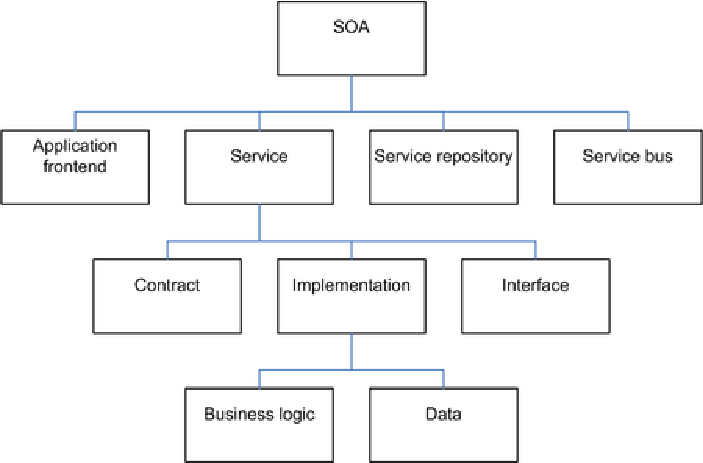
\includegraphics[scale=1]{soa_struct.pdf}
  \caption{ Структура протокола SOA. }
  \label{fig:domain:bayes_net}
\end{figure}

Программные комплексы, разработанные в соответствии с \foreignlanguage{english}{SOA} были реализованы как набор веб-служб, взаимодействующих по протоколу \foreignlanguage{english}{SOAP}. Интерфейсы компонентов в сервис-ориентированной архитектуре инкапсулируют детали реализации от остальных компонентов, таким образом, обеспечивая комбинирование и многократное использование компонентов для построения сложных распределённых программных комплексов, обеспечивая независимость от используемых платформ и инструментов разработки, способствуя масштабируемости и управляемости создаваемой системы.

Управление информацией между клиентским и серверным приложением осуществляется по REST протоколу. REST сервис полностью основывается на протоколе передачи данных. Для HTTP действие над данными задается с помощью методов: GET, PUT, POST, DELETE. Таким образом, действия CRUD могут выполняться как со всеми четырьмя методами, так и только с помощью GET и POST запросов~\cite{restfull}.

Основные возможности разработанного одностраничного приложения заключаются в написании одного сервиса по выдаче модели отображения и множества сервисов для взаимодействия пользователя с базой данных. Такие возможности заключаются в следующем:
\begin{enumerate}
  \item Пользователь получает возможность создавать личное хранилище, обладает уникальным идентификатором, который проверяется каждый раз, когда он совершает действия изменяющие состояние сервиса. Если конкретный пользователь пытается просмотреть записи хранилища, которое находится на в шифрованным виде, либо запись, которая принадлежит хранилищу доступного локально, его идентификатор поддается дешифровке и проверяется на валидность в рамках всего цикла жизни клиента.
  \item Пользователь может просматривать и редактировать определенные группы данных в хранилищах, дешифрованных его публичным ключом на клиенте, полученным при аутентификации. Добавлять новые поля и группы, имея авторизованный доступ к хранилищу.
  \item Пользователю предоставляется возможность добавлять, удалять и редактировать новые поля и хранилища. Создавать новые сертификаты доступа при утере или компрометации последних. Редактировать и восстанавливать доступ к поврежденным сертификатам.
  \item При редактировании записей, данные шифруются публичным ключом и отправляются на сервер, где подвергаются дешифровке приватным ключом и вторичному шифрованию синхронным методом.
\end{enumerate}

\subsection{Идентификация объектов предметной области}
\label{sub:domain:object}

В разрабатываемом приложении можно выделить четыре слоя, связанных между собой различными уровнями обструкции. И хотя у них есть общие части, такие, как модель данных, они вполне могут разрабатываться независимо друг от друга:
\begin{itemize}
  \item Client Layer;
  \item Application Server Layer;
  \item Business Layer;
  \item Data Layer.
\end{itemize}

Эта модель объединяет два основных слоя: Client Layer и \foreignlanguage{english}{Application Server Layer}. Таким образом, структура программы напоминает классическую трехуровневую модель~\cite[с.~308\,--\,401]{sicp_2006_ru}, в которой имеется три явно выраженных слоя. Пользовательский интерфейс, реализованный в Client Layer и \foreignlanguage{english}{Application Server Layer}, представляет собой блок отображения данных. Data Layer приложения, управляемый Business Layer, представляет собой уровень доступа к базе данных. Сюда относятся сервисы, которые поставляются драйвером СУБД, классы-посредники, и синглтоны. База данных представляет уровень Data, самый нижний уровень в иерархии.

Каждый из слоев имеет свой уровень абстракции, согласно которому каждый слой не знает о реализации другого. Все блоки работают по принципу черного ящика, каждому из которых необходимо лишь знать о входных и выходных параметрах. На основании этого можно более детально разобрать каждый элемент системы на подсистемы, поясняющие общий принцип взаимодействия модулей на разных слоях взаимодействия.

Business Layer представляет слой обработки пользовательских данных и событий Data Layer, обеспечивает высокоуровневый интерфейс для \foreignlanguage{english}{Application Server Layer}, скрывая реализацию Data Layer. Текущий слой обеспечивает связывание модулей, решает проблему связывания подписчиков и издателей путем автоматической регистрации событий, который автоматически вызывает нужные привязки на основе соглашения об именовании.
Существование Business Layer подразумевает регистрацию всех компонентов, которые могут подписываться на события, регистрацию всех событий на которые можно подписаться и набор событий компонентов.

Приемущество разработанной архитектуры связано с отсутствием зависимости между компонентами приложения. Это дает основание для формирования свободной иерархии пакетов, представляя возможность использовать разработанное приложение при построении более сложной архитектуры в качестве стороннего компонента или ядра. Кроме того, благодаря низкому уровню связанности кода, отдельные модули можно также использовать повторно в сторонних продуктах.

\subsection{Декомпозиция объектов предметной области}
\label{sub:domain:object_decomp}

На каждый логически выделенный слой программы возлагаются определенные задачи, решение которых делегируется сущностям более низкого порядка детализации. Кроме того, каждый блок программы так или иначе связан с остальными блоками, чтобы обеспечить работоспособность всего приложения в целом. Связь, как правило, реализуется посредством обмена данными утвержденной сигнатуры между блоками.

Блок пользовательского интерфейса представляет собой множество пользовательских компонентов, взаимодействующими между всеми остальными блоками программы. Он отвечает за отрисовку страницы в браузере. Основной его функцией является представление того или иного компонента пользователю по запросу от блока контроля и обработки событий. При этом он может обеспечивать рендеринг страницы из разных источников в рамках политики общего происхождения.

Блок контроля и обработки событий определяет наличие изменений состояния блоков пользовательского интерфейса и формирования запросов на сервер, производит оповещение подписчиков о текущем состоянии, служебных сообщениях, не относящиеся напрямую к работе текущего модулю. В первую очередь, это сообщения соединения с сервером, истечение срока действия авторизационный данных, системные ошибки во время исполнения процедур. Блок не имеет представления, как устроено отображение модели, и как работают сервисы, направленные на обновление модели. Блок контроля и обработки событий связан напрямую с блоком пользовательского интерфейса. Все действия и события, происходящие на странице, так или иначе обращаются к контроллеру. Контроллер, после обработки сервисом, возвращает обработанную модель событию на клиентской части, где происходит изменение отображения страницы.

Блок криптографической защиты данных представляет собой совокупность средств и методов шифрования/дешифрования различных типов данных, проверки электронной подписи и сбор данных для их дальнейшей обработки. Осуществляет весь спектор мероприятии по валидации данных и исправлению последствий неавторизованного доступа. Обладает полномочиями по разрыве связи с клиентом при попытке подмены сертификата, возобновление работы после замены старых ключей на новые.

Блок формирования запросов на сервер осуществляет имплементацию данных и их валидацию, а также формирование запросов к серверу соблюдая их иерархию. Все данные, которые отправляются с клиентской части на серверную, проходят проверку в текущем блоке. При соответствии сигнатуры, объекты данных передаются далее на сервер. Все правила, которым должна соответствовать модель, задаются на этапе разработки модели страницы и блоков валидации данных.

Блок серверной обработки HTTP-запросов представляет собой систему маршрутизации по принципу REST архитектуры. Основной причиной для ее внедрении послужило то, что большое количество логики на клиенте необходимо структурировать. К тому же в перспективе решение может масштабироваться. В этом случае возможно появление специальной клиентской части с ограниченным функционалом в качестве мобильного приложения. Не исключено появление и десктопных клиентов приложения. Приложение в основном использует JSON\footnote{\url{http://www.w3schools.com/json/}} для передачи информации и загрузки ее с сервера. Необходимость в максимальной расширяемости системы подразумевает, что к одной и той же точке API сервера могут подключаться разные версии приложения.

Блок обработки пользовательских событий на серверной стороне осуществляет проверку идентификационных данных пользователя, обеспечивая целостность и защиту от фальсификации передаваемой информации. Он может быть использован для обнаружения несанкционированных изменений данных, как преднамеренных, так и случайных, во время жизненного цикла приложения. Любая несанкционированная попытка получить доступ к данным посредствам неавторизованного подключения будет отклонена, а блок известит клиент о попытке несанкционированного доступа.

Блок базы данных представляет собой хранилище всей информации, с которой может работать приложение и пользователь. Блок реализует асинхронную репликацию в конфигурации, основанную на передаче журнала изменений с ведущего узла на ведомые, тем самым поддерживается автоматическое восстановление в случае выхода из строя ведущего узла. Принимает параметры, делает выборку или обновление записей в базе, согласно определенному сценарию, и возвращает набор данных, либо результат выполнения сервису приложения.

Блок объектной модели базы данных и блок обеспечения доступа к базе данных предоставляются драйвером СУБД на уровне платформы. Оба сервиса работают по принципу «черного ящика» – на вход передаются параметры, на выходе возвращаются данные.

\section{Функциональное проектирование} % (fold)
\label{sec:arch_and_mod}

\subsection{Описание конфигурации сборки проекта}
\label{sub:arch_and_mod:graphlib}

В отличие от большинства сборщиков проектов, приложение \npm{}\footnote{\url{https://www.npmjs.com/}} использует декларативный способ сборки проектов вместо императивного. Это значит, что \json{} файл содержит описание проекта, согласно которому данный проект собирается в исполняемый модуль платформы \nodejs{}.

В процессе построения проекта происходят следующие этапы:
\begin{itemize}
  \item синтаксический анализ – проверка на содержание файлом всех необходимых данных и на синтаксическую правильность. В данном пункте проверяется корректность декларативного описанию путем проверки с использованием \npmrc{};
  \item обработка ресурсов и создание основы приложения, загрузка из сети недостающих элементов, описанных в зависимостях;
  \item компиляция исходных файлов проекта, посредством TypeScriptCom"=piler и \typings{}\footnote{\url{https://github.com/typings/typings/}};
  \item обработка и компиляция тестов;
  \item тестирование – запуск тестов, только при успешно пройденных тестах выполняется следующий этап;
  \item формирование исполнительного модуля \nodejs{};
\end{itemize}

Тестовая среда, создаваемая после сборки проекта в исполняемый модуль, имеет все описанные в \json{} файле настройки. Файл package.json располагается в корневой директории проекта и является основным источником информации при запуске команд продукта \npm{}.

Общий вид файла, описывающий целый проект, содержит всю необходимую универсальному декларативному сборщику проектов \npm{} для формирования исполняемого модуля NodeJS и настройки тестовой среды для модуля расширения согласно описанных в файле настроек. Конфигурация исполнительного модуля приведена в листинге~\ref{lst:arch_and_mod:graph_definition}:
\begin{lstlisting}[style=json,caption={Конфигурация исполнительного модуля}, label=lst:arch_and_mod:graph_definition]
{
  "name": "password-manager",
  "description": "Password-manager of Artem Derevnjuk",
  "version": "0.1.2-rc.3",
  "main": "dist/passman.js",
  "author": "Artem Derevnjuk",
  "repository": {
    "type": "git",
    "url": "https://github.com/derevnjuk/passman.git"
  },
  "bugs": {
    "url": "https://github.com/cderevnjuk/passman /issues"
  },
  "keywords": [
    "passman",
    "password",
    "manager",
    "utility"
  ],
  "dependencies": {
    "body-parser": "^1.15.0",
    "express": "^4.13.4",
    "jsonwebtoken": "^5.7.0",
    "mongoose": "^4.4.8",
    "nconf": "^0.8.4",
    "promise": "^7.1.1",
    "node-uuid": "^1.4.2",
    "clone": "^0.1.19",
    "crypto-js": "^3.1.2",
  },
  "devDependencies": {
    "chai": "^3.1.0",
    "coveralls": "^2.11.2",
    "es6-promise": "^2.3.0",
    "fs-extra": "^0.26.7",
    "jscs": "^1.13.1",
    "jscs-jsdoc": "^1.3.2",
    "jshint": "~2.8.0",
    "karma": "^0.13.2",
    "karma-browserify": "^4.2.1",
    "karma-firefox-launcher": "^0.1.6",
    "karma-mocha": "^0.2.0",
    "karma-mocha-reporter": "^1.0.2",
    "mocha": "^2.2.5",
    "native-promise-only": "^0.8.0-a",
    "nodeunit": ">0.0.0",
    "nyc": "^2.1.0",
    "recursive-readdir": "^1.3.0",
    "rimraf": "^2.5.0",
    "rollup": "^0.25.0",
    "rollup-plugin-node-resolve": "^1.5.0",
    "rollup-plugin-npm": "~1.3.0",
    "rsvp": "^3.0.18",
    "semver": "^4.3.6"
  },
  "scripts": {
    "coverage": "nyc npm test && nyc report",
    "coveralls": "nyc npm test && nyc report --reporter=text-lcov | coveralls",
    "lint": "jshint lib/ test/ mocha_test/ perf/memory.js perf/suites.js perf/benchmark.js support/ karma.conf.js && jscs lib/ test/ mocha_test/ perf/memory.js perf/suites.js perf/benchmark.js support/ karma.conf.js",
    "mocha-browser-test": "karma start",
    "mocha-node-test": "mocha mocha_test/ --compilers js:babel-core/register",
    "mocha-test": "npm run mocha-node-test && npm run mocha-browser-test",
    "nodeunit-test": "nodeunit test/test-async.js",
    "test": "npm run-script lint && npm run nodeunit-test && npm run mocha-node-test"
  },
  "license": "MIT",
  "jam": {
    "main": "dist/passman.js",
    "include": [
      "dist/passman.js",
      "README.md",
      "LICENSE"
    ],
    "categories": [
      "Utilities"
    ]
  },
  "spm": {
    "main": "dist/passman.js"
  },
  "volo": {
    "main": "dist/passman.js",
    "ignore": [
      "**/.*",
      "node_modules",
      "bower_components",
      "test",
      "tests"
    ]
  }
}
\end{lstlisting}

Данный файл для сборщика \npm{} преобразуется неявно в совокупность свойств. Описание основных свойств файла программной модели описано ниже:
\begin{itemize}
  \item name, значение определяет уникальное имя пакета, пространство \\имен, общее для всех единиц исполняемого модуля;
  \item description, описание пакета, предоставляет исчерпывающую информацию по исполняемому модулю при его публикации;
  \item version, версия исполняемого модуля;
  \item main, точка входа в приложение, в тоже время идентификационное имя исполняемого модуля;
  \item author, информация об авторе и поставщике исполняемого модуля для платформы. Содержит такую информацию, как имя автора и ссылка на более подробную информацию о разработчике модуля;
  \item repository, публичный адрес на репозиторий в системе контроля версий,
  описывающий порядок доступа к проекту приложения;
  \item bugs, связывает bugs-tracking с системами автоматизированного обслуживания и отчетности;
  \item keywords, список ключевых слов для поиска пакета в менеджере пакетов;
  \item dependencies, список зависимостей, необходимых для корректного запуска приложения, набор описаний зависимых компонент модуля, описываются загружаемые в момент сборки компоненты, обеспечивающих основу модуля при сборке.
  \item devDependencies, список параметров пакетов рабочего окружения, который определяет набор исполняемых пакетов сборщик NPM, GULP и Sys"=temJS, необходимых для успешной сборки исполняемого модуля;
  \item scripts, словарь, содержащий скриптовые команды, которые запускаются во время жизни приложения по установленному условию;
  \item jam, список клиентских зависимостей, динамически внедряемых пакетов, необходимых для успешного запуска клиентского приложения.
  \item spm, статический идентификатор в системе пакетов SPM.
  \item volo, конфигурация конструктора модулей  AMD, CommonJS, Node.
\end{itemize}

В данном исполняемом модуле используются следующие компоненты и зависимости, описанные в dependencies:
\begin{itemize}
  \item body-parser – межпрограммный модуль обработки тела запроса, ответственный за разбор POST запросов от клиента;
  \item express – реактивный северный-фраймворк для \nodejs{}, предоставляющий основные элементы взаимодействия с функциональностью на стороне клиента посредством протокола SOAP. Содержит основной набор классов, необходимый для реализации REST-сервиса;
  \item jsonwebtoken – компонент, обеспечивающий аутентификацию по методу JSON Web Token\footnote{\url{https://jwt.io/}} со средствами хеширования JWT маркера;
  \item mongoose – система, которая предоставляет возможность объектно-реляционного отображения объектной модели приложения, в соответствии с интерфейсом NodeJS.
  \item nconf – основной компонент динамической конфигурации сервера на базе объектной модели. Является наиболее часто используемым компонентов взаимодействия сервера с нижестоящими слоями;
  \item promise – компонент спецификации ES2016\footnote{\url{https://github.com/tc39/ecma262}}, предоставляющий одни из рекомендуемых способов организации асинхронного кода
  \item node-uuid — модуль авторизации, поддерживающий JWT маркеры.
  \item clone — стандартный компонент многопроцессорного взаимодейст"=вия, производящий обмен данных между объектной моделью приложения и базой данных
  \item crypto-js — библиотека содержит реализацию функций шифрования и хеширования на северной и клиентской стороне.
\end{itemize}

В файл программной модели модуля могут также быть добавлены дополнительные свойства. При выполнении консольной команды npm run происходит полный цикл построение программного модуля, запуск тестов и запуск сервера \nodejs{} для работы тестовой среды приложения.
На программный модуль при использовании сборщика NPM накладывается ряд ограничений. Запуск команды npm run приводит к созданию в корневом каталоге папок node\_modules и typings, содержимое которых заполняется по мере выполнения команды. После успешного выполнения в папке node\_modules можно найти зависимости приложения и модуля тестирования данного программного средства, а также файлы тестовой среды для исполнительного модуля. Которые представляют собой одиночную версию разрабатываемого продукта в режиме быстрой разработки. Данный режим сканирует любые изменения исходного кода модуля и изменяет по мере выполнения функциональность определенных в модуле элементов. Эта возможность позволяет не перезапускать команду лишний раз при наличии изменений.

\subsection{Классы Business Layer}
\label{sub:arch_and_mod:probab_net}

К классам Business Layer относятся классы, наследующие от класса EventEmittor, который находится в пространстве имен NodeJS.events.EventE"=mittor. Основной ролью данных классов является формирования логики обработки всех декларированных объектов объектной модели во время жизненного цикла приложения в рамках асинхронной модели ввода\/вывода. Все классы принадлежащие этому слою являются реализацией интерфейса IBusinessSecu"=rityData.

\subsubsection{}
\label{sub:arch_and_mod:probab_net:observer}

Класс ObserverServer является базовым абстрактным классом для классов бизнес логики и наследует свойства и методы абстрактного класса EventEmittor. Класс не содержит дополнительных атрибутов и модификаторов доступа.

Поля:
\begin{itemize}
  \item \_logger – поле типа Logger, используется для логирования исключительных ситуаций, сбоев и отсутствие разрешений;
  \item applicationProperties – поле типа ApplicationProperties, позволяющее получить свойства текущей конфигурации ObserverServer;
  \item \_dataResultFactory – поле типа IDataResult, возвращающее выборку фабрики результатов, формирует модель результат валидации для дальнейшей передачи на слой выше.
\end{itemize}

Методы:
\begin{itemize}
  \item IObserverServer ObserverServer(ApplicationProperties applicationProper"=ties) – конструктор класса, принимающий в качестве параметров объект
  \item конфигурации;
  \item boolean \_hasAdminPermission() – метод, определяющий наличие прав на администрирование пользователей и групп. Метод используется для выполнения запросов к базе данных, предотвращая несанкционированные попытки получить пользовательские данные посредством не авторизованного доступа.
\end{itemize}

\subsubsection{}
\label{sub:arch_and_mod:probab_net:westley}

Класс Westley представляет собой класс, реализующий функционал редактора хранилища и менеджер истории его изменений. Является реализацией интерфейса IWestley.

Поля:
\begin{itemize}
  \item \_dataset – поле типа IStorageData исполнения процедуры в базе данных. На вход принимает модель запроса, на выходе возвращает результат выполнения процедуры;
  \item \_history – поле типа Array<IStorageHistory> контейнер истории для текущего пользователя;
  \item \_cachedCommands – поле типа Map<Command>, содержащая результаты наиболее частых запросов к хранилищу.
\end{itemize}

Методы:
\begin{itemize}
  \item IWestley clear() – метод возвращающий пустой объект хранилища.
  \item IWestley execute(Command command) – метод, принимает команды типа Command и делегирует их выполнение объекту command"=Tools типа ICommandTools, сохраняя историю и изменяя \_dataset.
  \item Command \_getCommadForKey(string commandKey) – метод возвращает command типа Command по переданному ключу из свойства \_cached"=Commands.
  \item IWestley pad() – метод возвращающий хранилище, внедряя смещение в оригинальный прототип хранилища.
  \item IStorageData getDataset() – метод возвращает результат выполнения процедуры в базе данных.
  \item Array<IStorageHistory> getHistory() – метод возвращает контейнер истории запросов к хранилищу.
\end{itemize}

\subsubsection{}
\label{sub:arch_and_mod:probab_net:archive}

Класс Archive управляет временем существования компоновкой и обработкой объектов ManagedEntry и ManagedGroup. Данный класс может иметь только один экземпляр для конкретного пользователя.

Поля:
\begin{itemize}
  \item \_westley – поле типа IWestley, инкапсулирует редактор хранилища и менеджер истории запросов к нему;
  \item date – поле типа Date, содержит дату создания экземпляра класса Archive.
\end{itemize}

Методы:
\begin{itemize}
  \item Archive() – конструктор класса;
  \item Array<ManagedEntry> findEntriesByCheck(Achive achive, string check, string key, RegExp value) – статический метод, возвращающий массив всех записей экземпляра класса Archive на основании переданных мета-значений;
  \item boolean containsGroupWithTitle(string groupTitle) – метод сопоставления всех существующих групп переданному заголовку группы;
  \item IManagedGroup createGroup(string title) – метод принимает имя группы в качестве аргумента и возвращает ее имплементацию;
  \item Array<IManagedGroup> findEntriesByMeta(string metaName, RegExp value) – метод сбора релевантной выборки групп по переданным, в качестве параметров, мета-данным и их значению типа string, и RegExp соответственно;
  \item Array<IManagedGroup> findEntriesByProperty(string property, RegExp value) – метод сбора релевантной выборки групп по переданным, в качестве параметров, свойству и его значению типа string, и RegExp соответственно;
  \item Array<IManagedGroup> findGroupsByTitle(string title) – метод поиска всех групп архива, которые соответствуют преданному имени title;
  \item IManagedEntry getEntryByID(string entryID) – метод, осуществляющий поиск записи по ее уникальному идентификатору;
  \item IManagedGroup getGroupByID(string groupID) – метод, который производит рекурсивный поиск по идентификатору группы;
  \item Array<ManagedGroup> getGroups() – метод возвращает все группы, которые содержит экземпляр класса Archive;
  \item ManagedGroup getTrashGroup() – метод, позволяющий получить удавленные группы, подписанные на экземпляр класса Archive;
  \item IWestley \_getWestley() – метод возвращает базовый экземпляр типа IWestley;
  \item Achive createWithDefaults() – метод, возвращающий экземпляр класса Archive c параметрами по умолчанию.
\end{itemize}

\subsubsection{}
\label{sub:arch_and_mod:probab_net:inigoCommand}

Класс InigoCommand представляет собой класс для обработки и выполнения команд типа Command, наследующий от статического класса REPL.

Поля:
\begin{itemize}
  \item \_commandKey – поле типа string, которое содержит индекс выполняемой команды;
  \item \_commnadArgs – поле типа Array<strign arg> вмещает набор аргументов команды;
  \item commandArgument – статическое поле типа Map<ItemMetaRoot>, хранит маркеры и идентификаторы, присвоенные Command по умолчанию;
  \item commands – статическое поле типа Map<Command>, описывающее все подписанные команды в рамках текущей реализации CommandArguments.
\end{itemize}

Методы:
\begin{itemize}
  \item InigoCommand() – конструктор класса;
  \item InigoCommand addArgument(...args) – метод принимает неизвестное количество аргументов, привязывая их к текущей выполняемой команде, возвращает
  \item объект типа InigoCommand;
  \item Command generateCommand() – метод возвращающий реализацию команды на основании полей \_commandKey и \_commnadArgs;
  \item InigoCommand create(string cmd) – статический метод, возвращающий один и только один экземпляр класса InigoCommand для единственной команды по переданному индексу.
\end{itemize}

\subsubsection{}
\label{sub:arch_and_mod:probab_net:managedgroup}

Класс ManagedGroup представляет собой класс для управления группами записей пользователя, наследующий от стандартного класса Stream. Определяет порядок привязки групп к хранилищам пользователя и подписку на события глобальной группы. Является реализацией интерфейса IManagedGroup.

Поля:
\begin{itemize}
  \item \_archive – поле типа string, которое содержит индекс выполняемой команды;
  \item \_westley – поле типа Array<string> вмещает набор аргументов команды;
  \item \_remoteObject – поле типа IremoteObject, содержащее ссылку на удаленную группу подписанную на события экземпляр ManagedGroup.
\end{itemize}

Методы:
\begin{itemize}
  \item ManagedGroup() – конструктор класса;
  \item ManagedEntry createEntry(string title) – метод создания новой записи с заголовком title, возвращающий экземпляр класса ManagedEntry;
  \item ManagedGroup createGroup(string title) – метод создания дочерний группы с именем title, возвращающий экземпляр класса;
  \item void delete() – метод удаления группы типа ManagedGroup и очистки \_westley и \_removeObject;
  \item ManagedGroup deleteAttribute(string attr) – метод удаления атрибута по переданному имени attr, возвращает ссылку на экземпляр класса
  \item ManagedGroup;
  \item string getAttribute(string attributeName) – метод принимает имя атрибута и возвращает значение релевантного атрибута типа string;
  \item Array<ManagedEntry> getEntries() – метод, возвращающий массив записей группы типа ManagedEntry, привязанной к экземпляру класса;
  \item Array<ManagedGroup> getGroup() – метод, возвращающий массив всех групп типа ManagedGroup привязанных к глобально группе;
  \item string getID() – метод возвращает идентификатор глобальной группы;
  \item string getTitle() – метод возвращает имя глобальной группы;
  \item boolean isTrash() – метод, осуществляющий проверку на тип группы, возвращает значение boolean;
  \item ManagedGroup moveToGroup(ManagedGroup group) – метод перемещения подчиненной группы в группу group, переданную в качестве параметра, возвращает ссылку на экземпляр класса;
  \item ManagedGroup setTitle(string title) – метод, который принимая заголовок группы типа string, устанавливает ее в качестве имени глобальной группы;
  \item ManagedGroup setAttribute(string attributeName, string value) – метод принимает имя свойства и его значения, присваивая его глобальной группе;
  \item IArchive \_getArchive() – метод возвращает реализацию интерфейса IArchive – владельца глобальной группы;
  \item IRemoteObject \_getRemoteObject() – метод, который возвращает значение поля remoteObject текущего экземпляра класса;
  \item IWestley \_getWestley() – метод, который возвращает значение поля \_westley в контексте экземпляра класса;
  \item ManagedGroup createNew(IArchive archive, string parentID) – статический метод, позволяющий создать новый экземпляр класса ManagedGroup в хранилище archive с ведущей группой, обладающей parentID.
\end{itemize}

\subsubsection{}
\label{sub:arch_and_mod:probab_net:managedentry}

Класс ManagedEntry используется для инициализации записи пользователя. Наследует свойства и методы абстрактного стандартного класса BaseManagementEntry. Имеет шаблон \_remoteObject для представления и инициализации функциональности на стороне клиента.

Поля:
\begin{itemize}
  \item \_archive – поле типа string, которое содержит индекс выполняемой команды;
  \item \_westley – поле типа Array<string> вмещает набор аргументов команды;
  \item \_remoteObject – поле типа IRemoteObject, содержащее ссылку на скрытый объект-токен, содержащий хранимую информацию.
\end{itemize}

Методы:
\begin{itemize}
  \item ManagedEntry(Archive archive, IRemoteObject remoteObj) – конструктор класса, в качестве параметров принимает экземпляр archive и ссылку на удаленное представление remoteObj;
  \item void delete() – метод удаляет запись, в случае, если запись уже удалена, полностью очищает все ссылки на нее;
  \item ManagedEntry deleteAttribute(string attr) – метод, удаляющий параметр записи, переданный в качестве единственного аргумента attr. Возвращает ссылку на текущий экземпляр записи типа ManagedEntry;
  \item ManagedEntry deleteMeta(string property) – метод удаляет метаданные по переданному параметру property. Возвращает ссылку на экземпляр на котором был вызван;
  \item string getAttribute(string attr) – метод возвращает значение параметра записи по преданному имени атрибута;
  \item DisplayInfo getDisplayInfo() – метод возвращает экземпляр класса Dis"=playInfo, который представляя объект типа JSON;
  \item MangedGroup getGroup() – метод возвращает ссылку на группу типы ManagedGroup, содержащий экземпляр текущей записи;
  \item string getMeta(string property) – метод возвращает мета-данные по ключу property;
  \item string getID() – метод, возвращающий идентификатор записи в качестве строки;
  \item string getProperty(string property) – метод возвращает значение свойства, переданного в качестве первого аргумента;
  \item ManagedEntry moveToGroup(ManagedGroup group) – метод позволяет переместить запись в группу, ссылку на которую принимает в качестве первого параметра;
  \item ManagedEntry setAttribute(string name, string value) – метод присваивает атрибут с именем name и значением value записи, возвращая ссылку на нее;
  \item ManagedEntry setProperty(string name, string value) – метод присваивает свойство с именем name и значением value записи, возвращая ссылку на нее;
  \item IArchive \_getArchive() – метод возвращает реализацию интерфейса IArchive, содержащего все записи и группы;
  \item IRemoteObject \_getRemoteObject() – метод, который возвращает значение поля remoteObject текущего экземпляра класса;
  \item IWestley \_getWestley() – метод, который возвращает значение поля \_westley в контексте экземпляра класса;
  \item ManagedEntry createNew(IArchive archive, string parentID) – статический метод, позволяющий создать новый экземпляр класса ManagedGroup в хранилище archive с ведущей группой, обладающей parentID.
\end{itemize}

\subsubsection{}
\label{sub:arch_and_mod:probab_net:credentials}

Класс Credentials используется для формирования и проверки прав доступа к хранилищам. Наследует свойства и методы абстрактного стандартного класса BaseManagementEntry.

Поля:
\begin{itemize}
  \item \_signing – поле типа Array<string> вмещает набор аргументов команды;
  \item \_model – поле типа IRemoteObject, содержащее ссылку на скрытый объект-токен, содержащий хранимую информацию.
\end{itemize}

Методы:
\begin{itemize}
  \item Credentials(Model data) – конструктор класса, в качестве единственного параметра принимает экземпляр типа Model;
  \item Credentials setIdentity(string username, string password) – метод устанавливает username и password поля \_model текущего экземпляра. Возвращает экземпляр класса Credentials;
  \item Credentials setType (CredentialsType type) – метод присваивает полномочия типа type, переданного в качестве первого параметра, модели поля \_model;
  \item Promise<IOcane> convertToSecureContent(string password) – метод преобразующий учетные данные в шифрованную строку посредством токена pass"=word. Возвращает Promise типа IOcane;
  \item Promise<IOcane> createFromSecureContent(IOcane content, password) – статический метод, возвращающий экземпляр класса Credentials, содержащий дешифрованные данные content.
\end{itemize}

\subsubsection{}
\label{sub:arch_and_mod:probab_net:certificate}

Класс Certificate используется для формирования и проверки подписи сертификата. Инкапсулирует логику по оптимизации вычислений больших простых чисел. Наследует свойства и методы абстрактного стандартного класса BaseManagementEntry.

Поля:
\begin{itemize}
  \item \_GCM – поле типа Buffer, содержит дополнительную информацию, используемую в качестве дополнительно параметра при проверки подлинности подписи;
  \item \_generator – поле типа IdiffieHellman, вмещает ссылку на генератор  Диффи-Хеллмана в кодировке поля \_GCM;
  \item digest – поле типа Int32Array, словарь описывающий форму хеширования данных для экземпляров класса EncodeForfatter;
  \item \_level – поле типа number, отражает количество итераций сдвига случайных кривых;
  \item \_timestamp – поле типа Date, содержит расчетное значение времени необходимого для осуществления шифрования;
  \item \_crypto – поле типа ICrypto, ссылка на композицию функций шифрования и хеширования.
\end{itemize}

Методы:
\begin{itemize}
  \item Certificate() – конструктор класса;
  \item Buffer exportChallenge(ISuperToken spkac) – метод, принимает аргумент типа ISuperToken, который вмещает в себя открытый ключ и проверку типа Сhallenge. Возвращает объект типа Buffer, инкапсулирующий переданный ключ и тайну;
  \item boolean verifySpkac(Buffer spkac) – метод осуществляет проверку на соответствие тайны и публичного ключа;
  \item Buffer getAuthTag() – метод возвращает тег аутентификации типа Buffer, прошедшего проверку подлинности шифрования;
  \item Buffer computeSecret(ISuperToken spkac) – метод принимает аргумент типа ISuperToken, на основании которого производит вычисление секрета по протоколу Диффи-Хеллмана. Возвращает секрет типа Buffer;
  \item IDiffieHellman getGenerator() – метод возвращает \_generator типа  IDif"=fieHellman;
  \item Buffer getPrime() – метод возвращает большое простое число типа Buffer;
  \item Buffer getPrivateKey() – метод возвращает приватный ключ типа Buffer;
  \item Buffer getPublicKey() – метод возвращает публичный ключ типа Buffer;
  \item void mac(Uint8Array message, Int32Array hmac) – метод, осуществляющий проверку подлинности хеш-функции hmac посредством переданного ключа message типа UInt8Array;
  \item Int32Array createMAC(Buffer password) – метод, позволяющий создать хеш-функцию для переданного пароля password типа Buffer;
  \item Buffer keyBlock(Uint8Array password, Uint8Array salt, number iteration, number blockIndex) – метод вычисления блока ключа для переданной соли типа Uint8Array и пароля password типа Uint8Array. Возвращает blockIndex блок ключа на итерации iteration, номер которой передан третьим параметром;
  \item Buffer compress(string data) – метод осуществляет декрементальный разбор данных и их сжатие по словарю. Возвращает сжатые данные типа Buffer;
  \item string decompress(Buffer data) – метод производит восстановление сжатых данных по словарю с их последующей нормализацией и смещением преобразующей формы с относительным смещением в форму с абсолютным;
  \item string normalizTextValue(string data) – метод нормализует данные после восстановления. Возвращает строку типа string;
  \item string getUniqueID() – метод возвращает индикатор среды распределенных вычислений, определяя уникальный флаг хранилища пользователя;
  \item string hashText(string data) – метод, осуществляющий хеширование данных типа string, переданных ему в качестве перового параметра;
  \item Buffer decideImpl(number iteration, number  blockIndex) – метод нормализует секрет Диффи-Хеллмана. Возвращает секрет типа Buffer;
  \item Buffer encrypt(Buffer data, Buffer key) – метод производит шифрование сжатых данных data по ключу key;
  \item Buffer decrypt(Buffer ciphertext, Buffer pubkey) – метод производит дешифрование сжатых данных ciphertext по публичному ключу pubkey.
  \item number \_nbi() – метод возвращает число типа BigInteger.
\end{itemize}

\subsection{Классы Data Layer}
\label{sub:arch_and_mod:data_layer}

К классам Business Layer относятся классы, наследующие от класса EventEmittor, который находится в пространстве имен NodeJS.events.Event"=Emittor. Основной ролью данных классов является формирования логики обработки всех декларированных объектов объектной модели во время жизненного цикла приложения в рамках асинхронной модели ввода\/вывода.

\subsubsection{}
\label{sub:arch_and_mod:data_layer:add_general_data_action}

Класс AddGeneralDataAction представляет собой класс, реализующий добавление новых записей в хранилище. Является реализацией интерфейса IDataAction.

Поля:
\begin{itemize}
  \item \_applicationContext – поле контекста приложения, содержит в себе информацию о текущем пользователе, локализации;
  \item \_dataResultFactory – поле фабрики результатов, формирует модель результат валидации для дальнейшей передачи на клиент;
  \item \_dataSourceInvoker – поле исполнения процедуры в базе данных. На вход принимает модель запроса, на выходе возвращает результат выполнения процедуры;
  \item \_partDetailQuoteHelper – поле класса помощника, выполняющего проверку на разрешение редактирования записи, и контейнера констант;
  \item \_quoteWizardSettings – контейнер настроек для текущего пользователя.
\end{itemize}

Методы:
\begin{itemize}
  \item AddGeneralDataAction() – конструктор класса;
  \item Task<IDataResult<PartDetailFormModel, PartDetailFormModel>> Proces"=sAsync(PartDetailFormModel contextModel) – метод, выполняющий обработку данных и запись этих данных в таблицу. На вход поступает модель, которую необходимо обновить, на выходе получается результат добавления.
\end{itemize}

\subsubsection{}
\label{sub:arch_and_mod:data_layer:add_misc_item}

Класс AddMiscItemDataAction представляет собой класс, реализующий добавление новых записей в таблицу Miscellaneous хранилища. Является реализацией интерфейса IDataAction.

Поля:
\begin{itemize}
  \item \_applicationContext – поле контекста приложения, содержит в себе информацию о текущем пользователе, локализации;
  \item \_dataResultFactory – поле фабрики результатов, формирует модель результат валидации для дальнейшей передачи на клиент;
  \item \_dataSourceInvoker – поле исполнения процедуры в базе данных. На вход принимает модель запроса, на выходе возвращает результат выполнения процедуры;
  \item \_partDetailQuoteHelper – поле класса помощника, выполняющего проверку на разрешение редактирования записи, и контейнера констант;
  \item \_quoteWizardSettings – контейнер настроек для текущего пользователя;
  \item \_updatePartDetailFormDataHelper – помощник для работы с сервисом запросов базы данных.
\end{itemize}

Методы:
\begin{itemize}
  \item AddMiskItemDataAction() – конструктор класса;
  \item Task<IDataResult<PartDetailFormModel, PartDetailFormModel>> Proces"=sAsync(PartDetailFormModel contextModel) – метод, выполняющий обработку данных и запись этих данных в таблицу. На вход поступает модель, которую необходимо обновить, на выходе получается результат добавления.
\end{itemize}

\subsubsection{}
\label{sub:arch_and_mod:data_layer:add_part_component}

Класс AddPartComponent представляет собой класс, реализующий добавление новых записей типа KeyComponent. Является реализацией интерфейса IDataAction.

Поля:
\begin{itemize}
  \item \_applicationContext – поле контекста приложения, содержит в себе информацию о текущем пользователе, локализации;
  \item \_dataResultFactory – поле фабрики результатов, формирует модель результат валидации для дальнейшей передачи на клиент;
  \item \_partDetailQuoteHelper – поле класса помощника, выполняющего проверку на разрешение редактирования записи, и контейнера констант;
  \item \_dataSourceInvoker – поле исполнения процедуры в базе данных. На вход принимает модель запроса, на выходе возвращает результат выполнения процедуры;
  \item \_quoteWizardSettings – контейнер настроек для текущего пользователя;
  \item \_updatePartDetailFormDataHelper – помощник для работы с сервисом запросов базы данных.
\end{itemize}

Методы:
\begin{itemize}
  \item AddPartComponent() – конструктор класса;
  \item Task<IDataResult<PartDetailFormModel, PartDetailFormModel>> Proces"=sAsync(PartDetailFormModel contextModel) – метод, выполняющий обработку данных и запись этих данных в таблицу. На вход поступает модель, которую необходимо обновить, на выходе получается результат добавления.
\end{itemize}

\subsubsection{}
\label{sub:arch_and_mod:data_layer:add_payments_routing}

Класс AddPaymentsRoutingDataAction представляет собой класс, реализующий добавление новых записей типа PaymentsRouting. Является реализацией интерфейса IDataAction.

Поля:
\begin{itemize}
  \item \_applicationContext – поле контекста приложения, содержит в себе информацию о текущем пользователе, локализации;
  \item \_dataResultFactory – поле фабрики результатов, формирует модель результат валидации для дальнейшей передачи на клиент;
  \item \_dataSourceInvoker – поле исполнения процедуры в базе данных. На вход принимает модель запроса, на выходе возвращает результат выполнения процедуры;
  \item \_partDetailQuoteHelper – поле класса помощника, выполняющего проверку на разрешение редактирования записи, и контейнера констант;
  \item \_quoteWizardSettings – контейнер настроек для текущего пользователя;
  \item \_updatePartDetailFormDataHelper – помощник для работы с сервисом запросов базы данных.
\end{itemize}

Методы:
\begin{itemize}
  \item AddPaymentsRoutingDataAction() – конструктор класса;
  \item Task<IDataResult<PartDetailFormModel, PartDetailFormModel>> Proces"=sAsync(PartDetailFormModel contextModel) – метод, выполняющий обработку данных и запись этих данных в таблицу. На вход поступает модель, которую необходимо обновить, на выходе получается результат добавления.
\end{itemize}

\subsubsection{}
\label{sub:arch_and_mod:data_layer:add_sub_component}

Класс AddSubComponentDataAction представляет собой класс, реализующий добавление новых полей типа SubKeyComponent. При вызове данный класс строит объект JSON, в котором содержатся поля, необходимые для добавления новой записи. Является реализацией интерфейса IDataAction.

Поля:
\begin{itemize}
  \item \_applicationContext – поле контекста приложения, содержит в себе информацию о текущем пользователе, локализации;
  \item \_dataResultFactory – поле фабрики результатов, формирует модель результат валидации для дальнейшей передачи на клиент;
  \item \_dataSourceInvoker – поле исполнения процедуры в базе данных. На вход принимает модель запроса, на выходе возвращает результат выполнения процедуры;
  \item \_partDetailQuoteHelper – поле класса помощника, выполняющего проверку на разрешение редактирования записи, и контейнера констант;
  \item \_quoteWizardSettings – контейнер настроек для текущего пользователя;
  \item \_updatePartDetailFormDataHelper – помощник для работы с сервисом запросов базы данных.
\end{itemize}

Методы:
\begin{itemize}
  \item AddSubKeyComponentDataAction () – конструктор класса;
  \item Task<IDataResult<PartCostDetailFormModel, PartCostDetailFormModel>> Pro"=cessAsync(PartCostDetailFormModel contextModel) – метод, выполняющий обработку данных и запись этих данных в таблицу. На вход поступает модель, которую необходимо обновить, на выходе получается результат добавления.
\end{itemize}

\subsubsection{}
\label{sub:arch_and_mod:data_layer:add_supply_item}

Класс AddSupplyItemDataAction представляет собой класс, реализующий добавление новых полей типа SupplyItemsKey. При вызове данный класс строит объект JSON, в котором содержатся поля, необходимые для добавления новой записи. Является реализацией интерфейса IDataAction.

Поля:
\begin{itemize}
  \item \_applicationContext – поле контекста приложения, содержит в себе информацию о текущем пользователе, локализации;
  \item \_dataResultFactory – поле фабрики результатов, формирует модель результат валидации для дальнейшей передачи на клиент;
  \item \_dataSourceInvoker – поле исполнения процедуры в базе данных. На вход принимает модель запроса, на выходе возвращает результат выполнения процедуры;
  \item \_partCostDetailQuoteHelper – поле класса помощника, выполняющего проверку на разрешение редактирования записи, и контейнера констант;
  \item \_quoteWizardSettings – контейнер настроек для текущего пользователя;
  \item \_updatePartCostDetailFormDataHelper – помощник для работы с сервисом запросов базы данных.
\end{itemize}

Методы:
\begin{itemize}
  \item AddSupplyItemDataAction() – конструктор класса;
  \item Task<IDataResult<PartCostDetailFormModel, PartCostDetailFormModel>> Pro"=cessAsync(PartCostDetailFormModel contextModel) – метод, выполняющий обработку данных и запись этих данных в таблицу. На вход поступает модель, которую необходимо обновить, на выходе получается результат добавления.
\end{itemize}

\subsubsection{}
\label{sub:arch_and_mod:data_layer:calculate_right_summary_totalst}

Класс CalculateRightSummaryTotalstDataAction представляет собой класс, реализующий пересчет итогового значения прав на все группы, составляющих его хранилище. Является реализацией интерфейса IDataAc"=tion.

Поля:
\begin{itemize}
  \item \_applicationContext – поле контекста приложения, содержит в себе информацию о текущем пользователе, локализации;
  \item \_dataResultFactory – поле фабрики результатов, формирует модель результат валидации для дальнейшей передачи на клиент;
  \item \_dataSourceInvoker – поле исполнения процедуры в базе данных. На вход принимает модель запроса, на выходе возвращает результат выполнения процедуры. Является экземпляром сервиса доступа к базе данных. Данное поле инициализируется на этапе запуска приложения с помощью контейнера;
  \item \_partCostDetailQuoteHelper – поле класса помощника, выполняющего проверку на разрешение редактирования записи, и контейнера констант;
  \item \_quoteWizardSettings – контейнер настроек для текущего пользователя;
  \item \_updatePartCostDetailFormDataHelper – помощник для работы с сервисом запросов базы данных.
\end{itemize}

Методы:
\begin{itemize}
  \item CalculateRightSummaryTotalstDataAction() – конструктор класса;
  \item Task<IDataResult<PartDetailFormModel, PartDetailFormModel>> Proces"=sAsync(PartDetailFormModel contextModel) – метод, выполняющий обработку данных и запись этих данных в таблицу. На вход поступает модель, которую необходимо обновить, на выходе получается результат добавления.
\end{itemize}

\subsubsection{}
\label{sub:arch_and_mod:data_layer:calculate_process}

Класс CalculateProcessDataAction представляет собой класс, реализующий учет действий пользователя, который был сконфигурирован пользователем. Является реализацией интерфейса IDataAction.

Поля:
\begin{itemize}
  \item \_applicationContext – поле контекста приложения, содержит в себе информацию о текущем пользователе, локализации;
  \item \_dataResultFactory – поле фабрики результатов, формирует модель результат валидации для дальнейшей передачи на клиент;
  \item \_dataSourceInvoker – поле исполнения процедуры в базе данных. На вход принимает модель запроса, на выходе возвращает результат выполнения процедуры;
  \item \_partCostDetailQuoteHelper – поле класса помощника, выполняющего проверку на разрешение редактирования записи, и контейнера констант;
  \item \_quoteWizardSettings – контейнер настроек для текущего пользователя;
  \item \_updatePartCostDetailFormDataHelper – помощник для работы с сервисом запросов базы данных.
\end{itemize}

Методы:
\begin{itemize}
  \item CalculateProcessDataAction () – конструктор класса;
  \item Task<IDataResult<PartDetailFormModel, PartDetailFormModel>> Proces"=sAsync(PartDetailFormModel contextModel) – метод, выполняющий обработку данных и запись этих данных в таблицу. На вход поступает модель, которую необходимо обновить, на выходе получается результат добавления.
\end{itemize}

\subsubsection{}
\label{sub:arch_and_mod:data_layer:calculate_accesses_user}

Класс CalculateAccessesUserDataAction представляет собой класс, реализующий оценку прав пользователя на доступ к хранилищам. Является реализацией интерфейса IDataAction.

Поля:
\begin{itemize}
  \item \_applicationContext – поле контекста приложения, содержит в себе информацию о текущем пользователе, локализации;
  \item \_dataResultFactory – поле фабрики результатов, формирует модель результат валидации для дальнейшей передачи на клиент;
  \item \_dataSourceInvoker – поле исполнения процедуры в базе данных. На вход принимает модель запроса, на выходе возвращает результат выполнения процедуры;
  \item \_partCostDetailQuoteHelper – поле класса помощника, выполняющего проверку на разрешение редактирования записи, и контейнера констант;
  \item \_quoteWizardSettings – контейнер настроек для текущего пользователя;
  \item \_updatePartCostDetailFormDataHelper – помощник для работы с сервисом запросов базы данных.
\end{itemize}

Методы:
\begin{itemize}
  \item CalculateProcessDataAction () – конструктор класса;
  \item Task<IDataResult<PartDetailFormModel, PartDetailFormModel>> Proces"=sAsync(PartDetailFormModel contextModel) – метод, выполняющий обработку данных и запись этих данных в таблицу. На вход поступает модель, которую необходимо обновить, на выходе получается результат добавления.
\end{itemize}

\subsubsection{}
\label{sub:arch_and_mod:data_layer:check_process_routing_delete}

Класс CheckProcessRoutingDeleteDataAction представляет собой класс, который проверяет возможность удаления записей с хранилища. Если процесс удалить не возможно, метод класса вернет валидационную ошибку с текстом сообщения. Иначе вернется результат успешной проверки, и запись будет удалена из базы данных. Является реализацией интерфейса IData"=Action.

Поля:
\begin{itemize}
  \item \_applicationContext – поле контекста приложения, содержит в себе информацию о текущем пользователе, локализации;
  \item \_dataResultFactory – поле фабрики результатов, формирует модель результат валидации для дальнейшей передачи на клиент;
  \item \_dataSourceInvoker – поле исполнения процедуры в базе данных. На вход принимает модель запроса, на выходе возвращает результат выполнения процедуры;
  \item \_partDetailQuoteHelper – поле класса помощника, выполняющего проверку на разрешение редактирования записи, и контейнера констант;
  \item \_quoteWizardSettings – контейнер настроек для текущего пользователя;
  \item \_updatePartDetailFormDataHelper – помощник для работы с сервисом запросов базы данных.
\end{itemize}

Методы:
\begin{itemize}
  \item CheckProcessRoutingDeleteDataAction () – конструктор класса;
  \item Task<IDataResult<PartDetailFormModel, PartDetailFormModel>> Proces"=sAsync(PartDetailFormModel contextModel) – метод, выполняющий проверку данных на наличие связей в базе данных. На вход поступает модель, которую необходимо проверить, на выходе получается валидационный результат;
\end{itemize}

\subsubsection{}
\label{sub:arch_and_mod:data_layer:get_part_detail}

Класс GetPartDetailDataAction представляет собой класс, который позволяет получить данные для модели на клиенте. Является реализацией интерфейса IDataAction.

Поля:
\begin{itemize}
  \item \_dataResultFactory – поле фабрики результатов, формирует модель результат валидации для дальнейшей передачи на клиент;
  \item \_partDetailQuoteHelper – поле класса помощника, выполняющего проверку на разрешение редактирования записи, и контейнера констант;
  \item \_getPartDetailFormDataHelper – помощник для работы с сервисом запросов базы данных для получения модели.
\end{itemize}

Методы:
\begin{itemize}
  \item GetPartDetailDataAction() – конструктор класса;
  \item Task<IDataResult<PartDetailFormModel, PartDetailFormModel>> Proces"=sAsync(PartDetailFormModel contextModel) – метод, выполняющий получающий данные для конкретной записи в базе данных. На вход поступает модель с ключами, на выходе получается модель типа Model.
\end{itemize}

\subsubsection{}
\label{sub:arch_and_mod:data_layer:view_part_detail}

Класс ViewPartDetailFormAction представляет собой главный класс, так называемую точку входа в приложение. Данный класс является фабрикой по формированию и наполнению модели данных на серверной стороне приложения. В приложении так же используются однотипные классы для формирования объектов отображения. Подобные классы являются реализацией интерфейса IViewAction. Единственным отличием между Managed"=Group и ManagedEntry является тип возвращаемой модели. Для ManagedGroup это ManagedGroupModel, для ManagedEntry – ManagedEntryModel.

Поля:
\begin{itemize}
  \item \_actionBarModelBuilderFactory – поле фабрики панели действий, формирует модель действий для дальнейшей передачи на клиент;
  \item \_partDetailQuoteHelper – поле класса помощника, выполняющего проверку на разрешение редактирования записи, и контейнера констант, выполняет роль контейнера, содержащего в себе текстовые константы и методы, которые необходимы для получения разрешений и настроек;
  \item \_getPartDetailFormDataHelper – помощник для работы с сервисом запросов базы данных для получения модели.
  \item \_ModelBuilder* – генератор классов-фабрик, которые возвращают конкретную модель для наполнения формы. В данном приложении используется два типа моделей: модели таблицы и модель формы, которая выступает контейнером для таблиц. Все такие классы принимают на вход модель данных, возвращают реализацию интерфейса ISectionViewModelBuilder.
\end{itemize}

Методы:
\begin{itemize}
  \item ViewPartDetailFormAction() – конструктор класса;
  \item Task<IDataResult<PartDetailFormModel, PartDetailFormModel>> \foreignlanguage{english}{ProcessAsync(PartDetailFormModel contextModel)} – метод, получающий данные для конкретной записи в базе данных, формирующий из этих данных контекстную модель, инициирующий модель отображения и наполняющий модель отображения секциями. На вход поступает модель с ключами, на выходе получается модель отображения;
\end{itemize}

\subsubsection{}
\label{sub:arch_and_mod:data_layer:view_part_detail}

Класс GetPartDetailFormDataHelper представляет собой класс, возвращающий данные хранилища по запросу пользователя.

Поля:
\begin{itemize}
  \item \_applicationContext – поле контекста приложения, содержит в себе информацию о текущем пользователе, локализации;
  \item \_dataSourceInvoker – поле исполнения процедуры в базе данных. На вход принимает модель запроса, на выходе возвращает результат выполнения процедуры;
  \item \_glossaryWordProvider – поле, позволяющее получить глосаризованное значение текстовых составляющих записей;
  \item \_quoteWizardSettings – контейнер настроек для текущего пользователя;
\end{itemize}

Методы:
\begin{itemize}
  \item GetPartDetailFormDataHelper () – конструктор класса;
  \item Task CalculateAccessUserModel contextModel) – метод калькуляции прав доступа к хранилищу;
  \item Task GetModelMarkupBreakdownData (Model contextModel) – метод получения данных для групп хранилища пользователя;
  \item Task GetLinkedInlineProcessRouting (Model contextModel) – метод метод получения данных для таблицы встроенных процессов;
  \item Task GetMarkupSummary (Model contextModel) – метод возвращающий реализацию объекта типа IMarkupData;
  \item Task GetPartDetailFormModelData (Model contextModel) – метод получения данных для формы, обладающий наибольшим приоритетом, вызывается в первую очередь;
  \item Task GetQuoteRaw(Model contextModel) – метод получения данных для таблицы с побочными полями текущей записи;
  \item Task CalculateMarkup (Model contextModel) – метод валидации, возвращающий оценочную стойкость пароля;
  \item Task GetGlossaryLabels (Model contextModel) – метод получения локализованных строковых литералов;
  \item Task GetPartDetailItems (Model contextModel) – метод получения данных для каждой записи текущей группы;
  \item Task GetPasswordRouting (Model contextModel) – метод получения паролей для конкретной записи;
  \item Task GetQuotePartComponents (Model contextModel) – метод составляющих компоненты в производственном цикле, вне виртуального событийного цикла слоя;
  \item Task SetEntrySummary(Model contextModel) – метод установки новой записи;
\end{itemize}

\subsubsection{}
\label{sub:arch_and_mod:data_layer:view_part_detail}

Класс UpdatePartDetailFormDataHelper представляет собой класс-сервис, обновляющий данные для страницы. Класс аналогичен предыдущему~\ref{sub:arch_and_mod:data_layer:view_part_detail}, за исключением того, что данные отправляются в базу, а не считываются.

Поля:
\begin{itemize}
  \item \_applicationContext – поле контекста приложения, содержит в себе информацию о текущем пользователе, локализации;
  \item \_dataSourceInvoker – поле исполнения процедуры в базе данных. На вход принимает модель запроса, на выходе возвращает результат выполнения процедуры;
  \item \_glossaryWordProvider – поле, позволяющее получить глосаризованное значение текстовых составляющих страницы;
  \item \_quoteWizardSettings – контейнер настроек текущего пользователя.
\end{itemize}

Методы:
\begin{itemize}
  \item UpdatePartDetailFormDataHelper() – конструктор класса;
  \item Task UpdateModelMarkupBreakdownData (Model contextModel) – метод обновления данных для групп хранилища пользователя;
  \item Task UpdateLinkedInlineProcessRouting (Model contextModel) – метод метод обновления данных для таблицы встроенных процессов;
  \item Task UpdateMarkupSummary (Model contextModel) – метод обновления реализации объекта типа IMarkupData;
  \item Task UpdatePartDetailFormModelData (Model contextModel) – метод обновления данных для формы, метод получения данных, обладающий наибольшим приоритетом, вызывается в первую очередь;
  \item Task UpdateQuoteRaw(Model contextModel) – метод обновления данных для таблицы с побочными полями текущей записи;
  \item Task UpdatePartDetailItems (Model contextModel) – метод обновления данных для каждой записи текущей группы;
  \item Task UpdatePasswordRouting (Model contextModel) – метод обновления процессов для конкретной записи;
  \item Task UpdateQuotePartComponents(Model contextModel) – метод обновления составляющих и компонент производственного процесса странице;
\end{itemize}

\subsection{Классы Application Server Layer}
\label{sub:arch_and_mod:application_server_layer}

К классам и методам сервисов относятся классы и методы, имеющие атрибуты @Path и принимающих в качестве параметра объект типа Request. Основной ролью данных классов и методов является формирования ответов для пользователя с целью дальнейшего взаимодействия через сервисы посредством AJAX. Методы сервиса являются основными методами влияния на среду выполнения приложения.

\subsubsection{}
\label{sub:arch_and_mod:application_server_layer:user-management-rest-resource}

Класс UserManagementRestResource используется для методов сервиса по управлению пользователями и группами. Добавлен атрибут @Path со значением /users. Является реализацией интерфейса IUserManagementSer"=vice.

Поля:
\begin{itemize}
  \item userUtil – поле типа UserUtil, хранящее менеджер пользователей приложения;
  \item groupManager – поле типа GroupManager, используется для логирования исключительных ситуаций, сбоев и отсутствие разрешений;
  \item logger – поле типа Logger, используется для логирования исключительных ситуаций, сбоев и отсутствие разрешений.
\end{itemize}

Методы:
\begin{itemize}
  \item UserManagementRestResource (UserUtil userUtil, GroupManager group"=Manager) – конструктор класса сервиса по управлению пользователями и группами, принимающего в качестве менеджер пользователей и менеджер групп;
  \item Response addUserToGroup(Request req) – метод сервиса, который добавляет пользователя к группе. Метод при успешном выполнении возвращает значение в формате JSON \lstinline!{"responseType": "Success", "message": ""}!.\\ Атрибут @Path имеет значение /addToGroup. Идентификаторы групп и пользователя передаются в качестве параметров HTTP запроса;
  \item Response moveUserFromGroup(Request req) – метод сервиса, который перемещает пользователя из одной группы в другую. Метод при успешном выполнении возвращает \lstinline!{"responseType": "Success", "message": ""}!. Атрибут @Path имеет значение /moveFromGroup. Идентификаторы групп и пользователя передаются в качестве параметров HTTP запроса;
  \item Response removeFromGroup(Request req) – метод сервиса, который удаляет пользователя из группы. Метод при успешном выполнении возвращает значение в формате JSON \lstinline!{"responseType": "Success", "message": ""}!. Атрибут @Path имеет значение /addToGroup. Идентификаторы групп и пользователя передаются в качестве параметров HTTP запроса;
  \item Response getUserInfo(Request req) – метод сервиса, который возвращает данные о конкретном пользователе. Метод при успешном выполнении возвращает сериализованный объект User в формате JSON . Атрибут @Path имеет значение /addToGroup. Идентификатор пользователя передаются в качестве параметра HTTP запроса.
\end{itemize}

\subsubsection{}
\label{sub:arch_and_mod:application_server_layer:label_management_rest_resource}

Класс LabelManagementRestResource используется для методов сервиса по управлению записями, группами и хранилищами. Добавлен атрибут @Path со значением /labels. Является реализацией интерфейса ILabel"=ManagementService.

Поля:
\begin{itemize}
  \item labelManager – поле типа LabelManager, хранящее менеджер записей приложения;
  \item issueManager – поле типа IssueManager, используется для логирования исключительных ситуаций, сбоев и отсутствие разрешений;
  \item logger – поле типа Logger, используется для логирования исключительных ситуаций, сбоев и отсутствие разрешений.
\end{itemize}

Методы:
\begin{itemize}
  \item LabelManagementAction(LabelManager labelManager, IssueManager \\issueManager) – конструктор класса сервиса по управлению записями, группами и хранилищами, менеджер записей и задач;
  \item Response addIssueToLabel(HttpServletRequest req) – метод сервиса, который добавляет группу к хранилищу. Метод при успешном выполнении возвращает значение в формате \lstinline!{"responseType": "Success", "message": ""}!.\\ Атрибут @Path имеет значение /addToLabel. Идентификатор задачи и значение метки передаются в качестве параметров HTTP запроса;
  \item Response moveIssueFromLabel(Request req) – метод сервиса, который удаляет записи с одной группы и добавляет к другой. Метод при успешном выполнении возвращает \lstinline!{"responseType": "Success", "message": ""}!. Атрибут @Path имеет значение /moveFromLabel. Идентификатор задачи и значение метки передаются в качестве параметров HTTP запроса;
  \item Response removeIssueFromLabel(Request req) – метод сервиса, который удаляет запись из группы. Метод при успешном выполнении возвращает значение в формате JSON \lstinline!{"responseType": "Success", "message": ""}!. Атрибут @Path имеет значение /removeFromLabel. Идентификатор задачи и значение метки передаются в качестве параметров HTTP запрос.
\end{itemize}

\subsubsection{}
\label{sub:arch_and_mod:application_server_layer:base_response}

Класс BaseResponse используются для взаимодействия с функциональностью клиента, сервисов и серверных элементов функциональных действий. Класс BaseResponse является базовым классом для любой сущности типа Application Server Layer.

Поля:
\begin{itemize}
  \item responseType – поле типа ResponseType, которое хранит статус ответа;
  \item message – поле строкового типа, которое используется для передачи сообщения об ошибке или для оповещения;
\end{itemize}

Методы:
\begin{itemize}
  \item BaseResponse() – конструктор класса базового ответа сервиса и функционального действия;
  \item BaseResponse(ResponseType responseType, String message) – перегрузка конструктора класса базового ответа сервиса и функционального действия с параметрами;
  \item getMessage() и setMessage(String message) – методы для получения и установки значения сообщения;
  \item getResponseType() и setResponseType(ResponseType responseType) – методы для получения и установки типа ответа сервиса и функционального действия.
\end{itemize}

\subsubsection{}
\label{sub:arch_and_mod:application_server_layer:quickmanagement}

Класс Quickmanagement является классом связи с сервисом и определяет события подписки на запросы пользователя.

Методы:
\begin{itemize}
  \item Quickmanagement addIssueToLabel(Array<string> ...options, Function callback) – метод асинхронного вызова метода addIssueToLabel сервиса Label"=ManagementService. Параметр options должен содержать идентификатор записи, идентификатор группы. В качестве значения параметра callback передается функция, которая будет вызвана после возврата ответа сервиса. Функция callback принимает в качестве параметра объект класса BaseResponse;
  \item Quickmanagement moveIssueFromLabel(Array<string> ...options, Fun"=ction callback) – метод асинхронного вызова метода moveIssueFromLabel сервиса LabelManagementService. Параметр options должен содержать идентификатор задачи, идентификаторы метки назначения и метки источника. В качестве значения параметра callback передается функция, которая будет вызвана после возврата ответа сервиса. Функция callback принимает в качестве параметра объект класса BaseResponse;
  \item Quickmanagement removeIssueFromLabel(Array<string> ...options, Fun"=ction callback) – метод асинхронного вызова метода removeIssueFromLabel сервиса LabelManagementService. Параметр options должен содержать идентификатор задачи, идентификаторы метки, из которой удаляется задача. В качестве значения параметра callback передается функция, которая будет вызвана после возврата ответа сервиса. Функция callback принимает в качестве параметра объект класса BaseResponse;
  \item Quickmanagement addUserToGroup(Array<string> ...options, Function callback) – метод асинхронного вызова метода addUserToGroup сервиса User"=ManagementService. Параметр options должен содержать идентификатор пользователя, идентификатор группы. В качестве значения параметра callback передается функция, которая будет вызвана после возврата ответа сервиса. Функция callback принимает в качестве параметра объект класса BaseResponse;
  \item Quickmanagement moveUserFromGroup(Array<string> ...options, Func"=tion callback) – метод асинхронного вызова метода moveUserFromGroup сервиса UserManagementService. Параметр options должен содержать идентификатор пользователя, идентификаторы группы назначения и группы источника. В качестве значения параметра callback передается функция, которая будет вызвана после возврата ответа сервиса. Функция callback принимает в качестве параметра объект класса BaseResponse;
  \item Quickmanagement removeFromGroup(Array<string> ...options, Functi"=on callback) – метод асинхронного вызова метода removeFromGroup сервиса UserManagementService. Параметр options должен содержать идентификатор пользователя, идентификатор пользователя, который удаляется из группы. В качестве значения параметра callback передается функция, которая будет вызвана после возврата ответа от сервиса. Функция callback принимает в качестве параметра объект класса BaseResponse;
  \item Quickmanagement getUserInfo(Array<string> ...options, Function call"=back) – метод асинхронного вызова метода getUserInfo сервиса UserManage"=mentService. Параметр options должен содержать идентификатор пользователя В качестве значения параметра callback передается функция, которая будет вызвана после возврата ответа от сервиса. Функция callback принимает в качестве параметра объект класса User;
  \item T parseResponse(Response response) – метод обработки ответа сервиса. Параметр response имеет значение ответа сервиса.
\end{itemize}

\section{Разработка программных модулей}
\label{sec:develop_modules}

\subsection{Алгоритм расчета апостериорной вероятности для оценки стойкости шифрования}
\label{sub:develop_modules:k2_algorithm}

В данном подразделе рассматривается известный алгоритм, использующий оценку апостериорной вероятности в качестве критерия поиска стойкой тайны для шифрования данных.
Подробное описание данной оценки и базового алгоритма поиска приведены в работе~\cite{Cooper1991}.

Существуют подходы, использующие байесов метод для оценки качества полученной тайны и алгоритмы на их базе пытаются максимизировать апостериорную вероятность структуры шифра для данного набора экспериментальны данных.
В программном обеспечении, разработанном в данном дипломном проекте, использовался критерий оценки качества структуры, приведенный в упомянутой выше работе.

В данном подразделе рассматривается принцип минимальной длинны описания\footnote{В англоязычной литературе используется термин minimum description length или сокращенно MDL.} и его применимость для задания функции оценки качества шифра.
Данный принцип позволяет среди множества моделей выбрать модель с оптимальным соотношением сложности и соответствием модели наблюдаемым данным.
Т.\,е. данный принцип позволяет выбрать несложную и <<полезную>> модель, устойчивую к проблеме переобучения\footnote{В англоязычной литературе данная проблема называется overfitting и подразумевает, что модель слишком хорошо объясняет данные на которых она обучалась, но из-за этого непригодна для прогнозирования "--- работе на данных ранее не известных.}.
Принцип минимальной длинны описания в своей нестрогой и наиболее общей формулировке гласит: среди множества моделей следует выбрать ту, которая позволяет описать данные наиболее коротко, без потери информации~\cite{Grunwald05atutorial}.
Условие отсутствия противоречий модели во входном потоке является необходимым признаком адекватной модели, но не является достаточным. Простейшей моделью, удовлетворяющей такому условию, будет модель, в которой неопределенность, создаваемая неизвестными параметрами, очень велика и позволяет согласовать модель не только с реальными срезами потока, но вообще с любыми наборами величин. Во всех известных авторам реализациях существует одна и та же дилемма: чем больше количество параметров в модели, тем она точнее описывает совокупность данных, но тем ниже надежды на то, что такая модель окажется адекватной. При уменьшении же числа параметров модели, уменьшается и ее практическая значимость, поскольку такая модель гораздо менее точно описывает данные.

В контексте поиска модели стойкого шифра, соответствующей экспериментальным данным, принцип минимальной длинны описания гласит, что нужно выбрать модель, которая минимизирует сумму длин кодирования самой модели и кодирования экспериментальных данных с помощью этой модели~\cite{Lam94learningbayesian}, что выражается формулой~(\ref{eq:develop_modules:k2_algorithm:description_length}):
\begin{equation}
  \label{eq:develop_modules:k2_algorithm:description_length}
  l(x^{R}[n]) = \min_{g \in G}\left[ l_{G}(g) + l_{g}(x^{R}[n]) \right] \text{\,,}
\end{equation}
\begin{explanation}
где & $ x^R $ & вектор размерностью $R$, содержащий значения переменных (атрибутов). Представлен как $ x^R =\newline= (x^{(1)}, x^{(2)}, \dotsc, x^{(R)} ) $, где атрибут $ x^{(j)} $ может принимать $ \alpha_{j} $ значений, $ j = 1,\dotsc,R.$ \\
    & $ n $ & количество случаев в экспериментальных данных;  \\
    & $ x^R[n] $ & набор экспериментальны данных; \\
    & $ G $ & множество моделей; \\
    & $ l_{G}(g) $ & длина описания модели; \\
    & $ l_{g}(x^{R}[n]) $ & длина представления данных $ x^R[n] $ моделью $ g \in G $.
\end{explanation}

Для вычисления длинны кодирования модели и длинны кодирования данных с использованием модели в реализации дипломного проекта использовались результаты, приведенные в работах~\cite{Suzuki93,terentyev_2006}.
Собственно модель вероятностной сети состоит из таблиц условных и безусловных распределений и отношений <<родитель"=потомок>> между вершинами.
Для вычисления длины кодирования модели можно воспользоваться формулой~(\ref{eq:develop_modules:k2_algorithm:model_length}):
\begin{equation}
  \label{eq:develop_modules:k2_algorithm:model_length}
  l_{G}(g) = \frac{\log{n}}{2} \cdot \sum_{k = 1}^{R} S_k(g) (\alpha_k - 1) \text{\,,}
\end{equation}
\begin{explanation}
где & $ S_k(g) $ & количество возможных назначений переменных"=родителей переменной $X_k$, способ вычисления данного значения отличается у классических шифров и их модификации.
\end{explanation}

Введем некоторые обозначения, в дополнение к тем, которые были введены в подразделе~\ref{eq:develop_modules:k2_algorithm:description_length}.
Пусть структура шифра обозначается символом $B_S$, таблицы условных распределений, ассоциированные с ним, "--- $B_P$.
\newpage
Две вероятностные сети для данного набора экспериментальных данных можно оценить по отношению~(\ref{eq:develop_modules:k2_algorithm:nets_ratio}) апостериорных вероятностей:
\begin{equation}
  \label{eq:develop_modules:k2_algorithm:nets_ratio}
  \frac{P(B_{S_i} | x^R[n])}{P(B_{S_j} | x^R[n])} =
    \frac{ \frac{P(B_{S_i}, x^R[n])}{P(x^R[n])} }
         { \frac{P(B_{S_j}, x^R[n])}{P(x^R[n])} } =
    \frac{ P(B_{S_i}, x^R[n]) }
         { P(B_{S_j}, x^R[n]) } \text{\,.}
\end{equation}

Как видно из приведенной формулы~(\ref{eq:develop_modules:k2_algorithm:nets_ratio}), научившись вычислять отношение совместных распределений, можно сравнивать апостериорные вероятности структур вычисляемых шифров.
Т.\,к. в разработанном ПО использовались результаты, приведенные в работе~\cite{Cooper1991}, то считаем целесообразным привести в данном подразделе базовые формулы и предположения из вышеупомянутой работы.

Для вычисления $P(B_S, D)$ важно сделать несколько важных предположений:

\begin{enumerate}
  \item
  Экспериментальные данные содержат только дискретные случайные величины и все эти случайные величины присутствуют в истинной структуре $B_S$ модели из которой были получены эти экспериментальные данные.
  Из данного предположения следует формула~(\ref{eq:develop_modules:k2_algorithm:assumption1}):
  \begin{equation}
    \label{eq:develop_modules:k2_algorithm:assumption1}
    \int_{B_P} P(x^R[n] | B_S, B_P) f(B_P | B_S) P(B_S) dB_p \text{\,,}
  \end{equation}
  \par\hspace{\fivecharsapprox} % абзацный отступ
  \begin{tabular}{@{}ll@{ --- }p{0.74\textwidth}}
  где & $ B_P $ & вектор, содержащий значения условных вероятностей для назначений переменных из структуры $ B_S $; \\
      & $ f $ & условная плотность распределения $B_P$ при условии структуры $B_S$. \\[\parsep]
  \end{tabular}

  \item
  Случаи, зафиксированные в экспериментальных данных, независимы друг от друга, при условии зафиксированной модели, т.\,е. данное предположение подразумевает, что модель, генерирующая экспериментальные данные не меняется.
  Это предположение позволяет упростить формулу~(\ref{eq:develop_modules:k2_algorithm:assumption1}) и привести её к виду:
  \begin{equation}
    \label{eq:develop_modules:k2_algorithm:assumption2}
    P(B_S, x^R[n]) =
      P(B_S) \int_{B_P} \left[ \prod_{j = 1}^{n} P(x^R_j | B_S, B_P) \right] f(B_P | B_S) dB_P \text{\,.}
  \end{equation}

  \item
  Экспериментальные данные не должны содержать пропущенных значений для переменных из структуры $B_S$.
  Введем дополнительные обозначения.
  Пусть $x_j^{(i)}$ представляет значение $i$-й переменной в $j$-м случае.
  Пусть $\phi_i$ представляет из себя вектор уникальных назначений переменных"=родителей для $i$-й переменной, т.\,е. вектор уникальных назначений для $ \forall X_k,\ k \in \pi_i$.
  Пусть $\sigma(i, j)$ индексная функция, которая возвращает индекс назначения $\pi_i$ в $j$-ом случае из вектора $\phi_i$.
  Введем обозначение для длинны вектора $q_i = | \phi_i |$.
  Теперь с учетом предположения об отсутствии пропущенных значений можно вычислить вероятность конкретного случая из экспериментальных данных по формуле:
  \begin{equation}
    \label{eq:develop_modules:k2_algorithm:case_prob}
    P(x^R_j | B_S, B_P) =
      \prod_{i = 1}^{R} = P(X_i = x_j^{(i)} | \phi_i[\sigma(i, j)], B_P) \text{\,.}
  \end{equation}
  Подставляя выражение~(\ref{eq:develop_modules:k2_algorithm:case_prob}) в формулу~(\ref{eq:develop_modules:k2_algorithm:assumption2}) получим:
  \begin{align}
    \label{eq:develop_modules:k2_algorithm:assumption3}
    P(B_S, x^R[n]) =
      P(B_S)
      \int_{B_P}\left[ \prod_{j = 1}^{n}\prod_{i = 1}^{R} P(X_i = x_j^{(i)} | \phi_i[\sigma(i, j)], B_P)  \right] &\times \notag\\
      \times f(B_P | B_S) dB_P \text{\,.}
  \end{align}
  Пусть для выбранных $i$ и $j$ $f(P(x_i | \phi_i[j], B_P))$ обозначает плотность распределения возможных значений $P(x_i | \phi_i[j], B_P)$.
  Необходимо сделать еще одно предположение.

  \item Для $ 1 \le i, i' \le n$, $ 1 \le j \le q_i $, $1 \le j' \le q_i $, если
  $ij \neq i'j'$, то распределение $f(P(x_i | \phi_i[j]))$ не зависимо от распределения $f(P(x_{i'} | \phi_{i'}[{j'}]))$.
  Данное предположение по свой сути полагает, что до того, как были получены экспериментальные данные, все возможные назначения равновероятны.
\end{enumerate}

С учетом приведенных выше предположений и теоремы, приведённой и доказанной в работе~\cite{Cooper1991}, можно привести формулу для вычисления $P(B_S, D)$:
\begin{equation}
  \label{eq:develop_modules:k2_algorithm:model_and_data_prob}
  P(B_S, x^R[n]) =
    P(B_S)
    \prod_{i = 1}^{R}
    \prod_{j = 1}^{q_i}
    \frac{(\alpha_i - 1)!}
         {(n[\phi_i[j], i, B_S] + \alpha_i - 1)!}
    \prod_{k = 1}^{\alpha_i}
      n[v_{ik}, \phi_i[j], i, B_S]! \text{\,,}
\end{equation}
\par
\begin{tabular}{@{}ll@{ --- }p{0.74\textwidth}}
где & $ v_{ik} $ & $k$-е возможное назначение переменной $X_i$. \\[\parsep]
\end{tabular}

Формула~(\ref{eq:develop_modules:k2_algorithm:model_and_data_prob}) позволяет вычислить значение $P(B_S, x^R[n])$, если известна вероятность $P(B_S)$ и подсчитана оставшаяся часть формулы на основе экспериментальны данных $x^R[n]$.
Но из-за того, что $P(B_S)$ является чаще неизвестной величиной, чем известной, предполагают, что все возможные структуры сети равновероятны и $P(B_S)$ является некой малой константой.
Апостериорную вероятность структуры можно вычислить по формуле~(\ref{eq:develop_modules:k2_algorithm:aposteriori_structure_given_data}):
\begin{equation}
  \label{eq:develop_modules:k2_algorithm:aposteriori_structure_given_data}
  P(B_S | x^R[n]) =
    \frac{P(B_S, x^R[n])}
         {\sum_{B_S}P(B_S, x^R[n])} \text{\,.}
\end{equation}

Но, как уже упоминалось, множество возможных структур слишком велико, и на практике значение апостериорной вероятности можно вычислить лишь для шифров данных малой длины.

Формулу~(\ref{eq:develop_modules:k2_algorithm:model_and_data_prob}) для оценки совместной вероятности на практике напрямую использовать не получится, без введения дополнительных предположений.
Необходимо сделать предположение, что все возможные структуры равновероятны, т.\,е. $P(B_S)$ равно некоторой малой константе $c$.
Таким образом нахождение оптимальной структуры сводится к максимизации формулы~(\ref{eq:develop_modules:k2_algorithm:optimization_objective}), т.\,e. задача сводится к нахождению множества вершин"=предков $ \pi_i $ для каждой вершины $X_i$, оптимизирующих целевую функцию~\cite{Cooper1991}.
\begin{align}
  \label{eq:develop_modules:k2_algorithm:optimization_objective}
  \max \left[ P(B_S, x^R[n]) \right] = \notag\\
  =
    c \prod_{i = 1}^{R} \max_{\pi_i}
    \bigg[
      \prod_{j = 1}^{q_i} &% to align formula
      \frac{(\alpha_i - 1)!}
           {(n[\phi_i[j], i, B_S] + \alpha_i - 1)!}
      \prod_{k = 1}^{\alpha_i}
        n[v_{ik}, \phi_i[j], i, B_S]!
    \bigg] \text{\,.}
\end{align}

Таким образом наивный алгоритм поиска состоит в полном переборе всех возможных родителей для каждой вершины и оптимизации при этом функции~(\ref{eq:develop_modules:k2_algorithm:node_optimization_obj}):
\begin{equation}
  \label{eq:develop_modules:k2_algorithm:node_optimization_obj}
  g(i, \pi_i) =
    \prod_{j = 1}^{q_i}
      \frac{(\alpha_i - 1)!}
           {(n[\phi_i[j], i, B_S] + \alpha_i - 1)!}
      \prod_{k = 1}^{\alpha_i}
        n[v_{ik}, \phi_i[j], i, B_S]! \text{\,.}
\end{equation}

На практике наивный вариант не годится из-за большого количества возможных вариантов структур шифров.
В разработанной реализации использовались те же ограничения и стратегия поиска, что и в работе~\cite{Cooper1991}.
Перед началом выполнения алгоритма требуется знание о порядке вершин, таком, что вершины родители всегда находятся раньше вершин потомков.
Схематически алгоритм поиска выглядит следующим образом:

\begin{lstlisting}[style=fsharpstyle,escapeinside={/*@}{@*/},caption={Псевдокод реализации алгоритма К2}, label=lst:arch_and_mod:k2_algorithm:k2_pseudo]
function k2 =
  (* Input: dataset $x^R[n]$, ordering of variables, u - maximum number of parents per variable.
     Output: for each node, a printout of the parents of the node. *)
  for i in 1 .. R do
    $ \pi_i $ := $ \emptyset $
    $P_{old}$ := $g(i, \pi_i)$; // formula(/*@\ref{eq:develop_modules:k2_algorithm:node_optimization_obj}@*/)
    OkToContinue := true;
    while OkToContinue and $|\pi_i| < u$ do
      let z = node in $ \text{Pred}(X_i) - \pi_i $ that maximizes $ g(i, \pi_i \cup {z}) $
      $P_{new}$ := $f(i, \pi_i \cup {z})$
      if $P_{new} > P_{old}$ then
        $P_{old}$ := $P_{new}$;
        $ \pi_i $ := $ \pi_i \cup {z} $
      else OkToContinue := false
    end while
    printfn("Node: ", $X_i$, "Parents of $X_i$:", $\pi_i$)
  end for
end
\end{lstlisting}

В разработанной в рамках дипломного проекта реализации за основу был взят алгоритм К2, приведенный в работе~\cite{Cooper1991}, псевдокод которого показан в листинге~\ref{lst:arch_and_mod:k2_algorithm:k2_pseudo}.
В разработанном алгоритме слегка изменен способ подсчета целевой функции.
Приняв во внимание ограничение задания на дипломное проектирование, а также то, что операции умножения, деления и возведения в степень более сложные, было принято решение воспользоваться прологарифмированной версией формулы~(\ref{eq:develop_modules:k2_algorithm:node_optimization_obj}).

В качестве оценки степени зависимости двух произвольных переменных в работе~\cite{Chow68approximatingdiscrete} было предложено использовать значение взаимной информации\footnote{В англоязычной литературе используется термин mutual information}.
Эта информация задаёт приоритет поиска зависимостей между переменными.
По своей сути значение обоюдной информации является аналогом корреляции, но по своему содержанию "--- это оценка количества информации содержащейся в одной переменной о другой~\cite{terentyev_2006}.
Значение взаимной информации принимает неотрицательные значения и равно нулю в случае независимости случайных величин.
Для вычисления взаимной информации была предложена формула~(\ref{eq:develop_modules:k2_algorithm:mutual_information}):
\begin{equation}
  \label{eq:develop_modules:k2_algorithm:mutual_information}
  I(X; Y) = \sum_{y \in Y} \sum_{x \in X}
                 p(x, y) \log{ \left(\frac{p(x, y)}{p(x)\,p(y)}
                              \right) } \text{\,,}
\end{equation}
\begin{explanation}
где & $ p(x, y)$ & совместное распределение случайных величин $X$ и $Y$; \\
    & $ p(y) $ & безусловное распределение случайной величины $X$; \\
    & $ p(x) $ & безусловное распределение случайной величины $Y$.
\end{explanation}

Ниже приводится точная формула~(\ref{eq:develop_modules:k2_algorithm:log_node_optimization_obj}), по которой вычисляется оценка в реализованном алгоритме на основании формулы~(\ref{eq:develop_modules:k2_algorithm:mutual_information}), предложенной в работе~\cite{Chow68approximatingdiscrete}.
Данная формула более удобная для вычисления на платформе разработки, указанной в задании на дипломное проектирование:
\begin{align}
  \label{eq:develop_modules:k2_algorithm:log_node_optimization_obj}
  \log(g(i, \pi_i)) &=
    \sum_{j = 1}^{q_i}
      \log
      \left(
        \frac{(\alpha_i - 1)!}
             {(n_{ij} + \alpha_{i} - 1)!}
        \prod_{k = 1}^{\alpha_i}
          n_{ijk}!
      \right) =\notag\\
    &=
    \sum_{j = 1}^{q_i}
      \left(
        \log
          \frac{(\alpha_i - 1)!}
               {(n_{ij} + \alpha_{i} - 1)!}
        +
        \log
          \prod_{k = 1}^{\alpha_i}
            n_{ijk}!
      \right) =\notag\\
    &=
    \sum_{j = 1}^{q_i}
      \left(
        \log (\alpha_i - 1)! - \log (n_{ij} + \alpha_{i} - 1)!
        +
        \sum_{k = 1}^{\alpha_i}
          \log n_{ijk}!
      \right) =\notag\\
    &=
      \sum_{j = 1}^{q_i}
      \left(
        \log \Gamma(\alpha_i) - \log \Gamma(n_{ij} + \alpha_{i})
        +
        \sum_{k = 1}^{\alpha_i}
          \log \Gamma(n_{ijk} + 1)
      \right) = \notag\\
    &=
      q_i \log \Gamma(\alpha_i) +
      \sum_{j = 1}^{q_i}
      \left(
        \sum_{k = 1}^{\alpha_i}
          \log \Gamma(n_{ijk} + 1)
        - \log \Gamma(n_{ij} + \alpha_{i})
      \right) \text{\,,}
\end{align}
\begin{explanation}
где & $ \Gamma $ & гамма-функция "---  расширение понятия факториала на поле комплексных чисел; \\
    & $ n_{ijk} $ & условное, более краткое, обозначение для $n[v_{ik}, \phi_i[j], i, B_S]$; \\
    & $ n_{ij} $ & условное, более краткое, обозначение для $n[\phi_i[j], i, B_S]$.
\end{explanation}

Помимо использования формулы~(\ref{eq:develop_modules:k2_algorithm:log_node_optimization_obj}) в реализации были произведены дополнительные оптимизации, продиктованные результатами профилирования реализации алгоритма, изложенные в подразделе~\ref{sub:develop_modules:class}.

\subsection{Классификатор нормализации данных}
\label{sub:develop_modules:class}

Класс \foreignlanguage{english}{Certificate} использует большие простые числа для формирования классификатора. Время обработки каждого члена классификатора, содержащего числа высокой разрядности затруднено проблемами факторизации~\cite{facto_number}. Для сокращения времени обработки и вычисления тайны, базовые операции компрессии и нормализации данных были разбиты на каскады простых операций, формализованных асинхронными методами.

Каскады объединяются в каскады классификаторов. Процесс анализа членов сводится к тому, что простые числа последовательно анализируется на каждом каскаде классификатора, получая уникальную порцию примеси и смещения. При этом на каждом этапе происходит отсеивание некоторого количества разрядов, которые на последующих стадиях обрабатываться уже не будут. После того, как тайна пройдет через все каскады классификатора, выдается результат.

Однако из-за того, что прототип тайны имеет фиксированный размер, каждый член классификатора был снабжен вторым уникальным хеш-ключем, который по размеру соответствуют анализируемой области. Для создания тайны произвольного размера применяется два подхода: либо масштабирование классификатора, либо масштабирование самой тайны.

Структуру классификатора, который используется в программе генерации тайны, графически можно изобразить как на рисунке~\ref{fig:develop_modules:class:class_default}.

\begin{figure}[ht]
\centering
  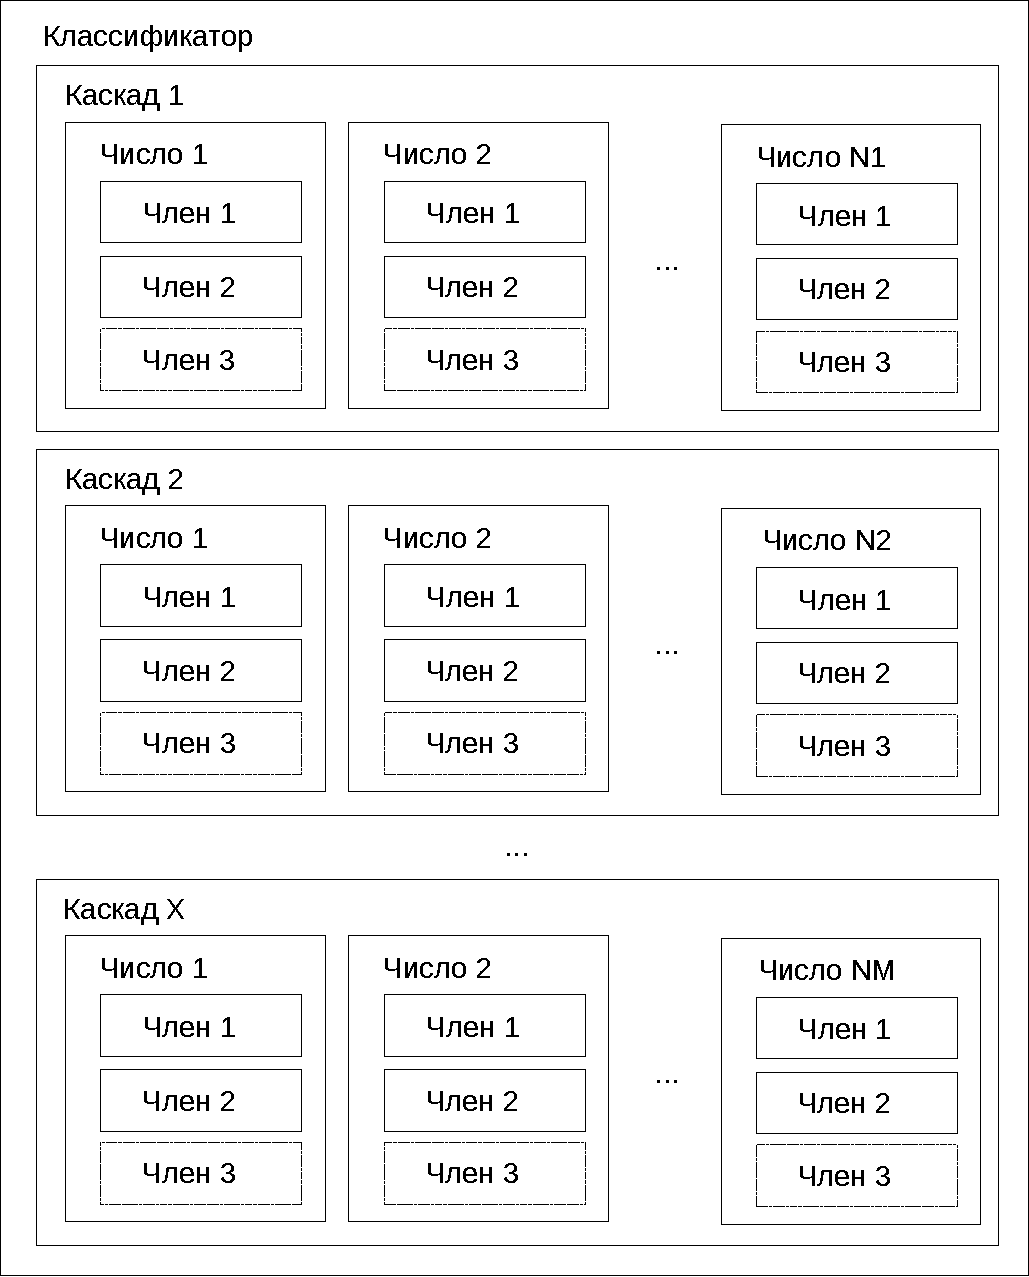
\includegraphics[scale=0.5]{class_default.pdf}
  \caption{ Структура классификатора. }
  \label{fig:develop_modules:class:class_default}
\end{figure}

Как видно из данного рисунка, классификатор состоит из множества каскадов, в каждый из которых входит набор чисел. Каждое число определяет два или три члена (так как третье член может отсутствовать, оно отмечено штрихом). Однако такая структура не является оптимальной, потому что она требует лишние операции над членами при работе. Поэтому была разработана структура, которая минимизирует число операций, на ряду с обфускацией связей между ними. Она изображена на рисунке~\ref{fig:develop_modules:class:class_changed}.

\begin{figure}[ht]
\centering
  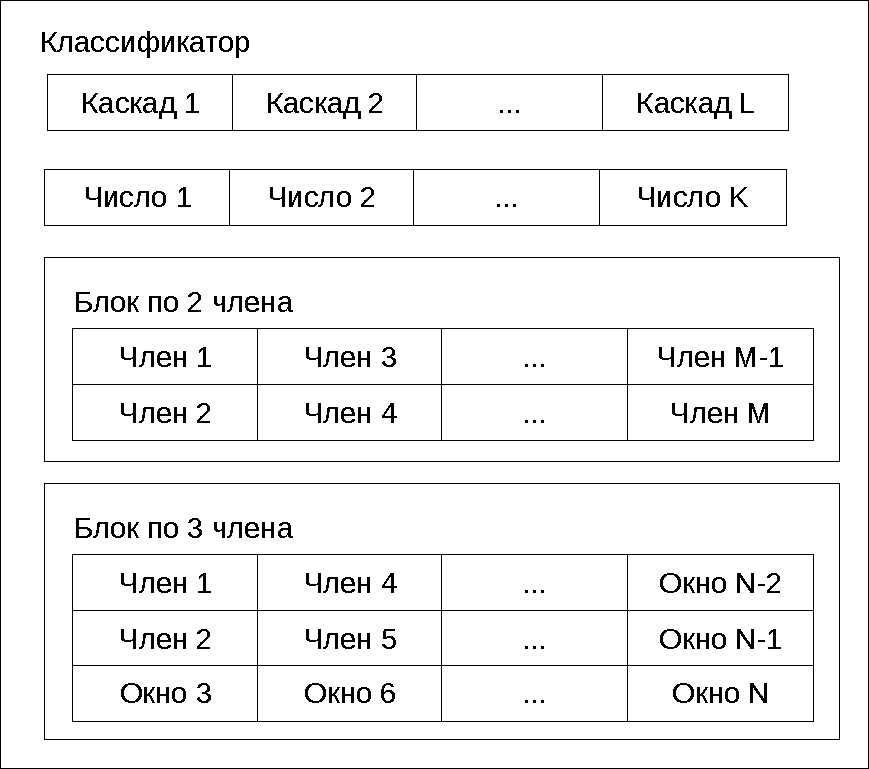
\includegraphics[scale=0.6]{class_changed.pdf}
  \caption{ Минимизированная структура классификатора }
  \label{fig:develop_modules:class:class_changed}
\end{figure}

\newpage

Для описания классификатора на рисунке~\ref{fig:develop_modules:class:class_changed} были разработаны следующие структуры:
\begin{lstlisting}[style=fsharpstyle,escapeinside={/*@}{@*/},caption={Структуры классификатора}, label=lst:develop_modules:class:structurs]
enum number_cascade {
  UInt32Array<number> node2_count,
  UInt32Array<number> node2_first,
  UInt32Array<number> node3_count,
  UInt32Array<number> node3_first,
  UInt32Array<number> node_position,
  Float32Array<number> threashold
};

enum number_rect {
  UInt8ClampedArray<number> p1,
  UInt8ClampedArray<number> p2,
  UInt8ClampedArray<number> p3,
  UInt8ClampedArray<number> p4
};

enum number_node {
  number a;
  number b;
  Float32Array<number> threashold;
};
\end{lstlisting}

Структура number\_cascade соответствует описанию каскадов. Так как все числа и члены располагаются линейно без разделения на каскады, структура должна содержать индексы начала блоков по два члена node2\_first, по три члена node3\_first и начало блока чисел node\_position. Также, чтобы упростить вычисления, введено число членов по два node2\_count и по три no"=de3\_count, количество чисел для данного каскада определяется как сумма блоков по два и три члена. Переменная threashold используется для принятия окончательного решения – подходит или нет данная область.
Все окна описывает структура number\_rect. Ее элементы описывают смещение относительно членов, который рассматривается в текущий момент данным вычислительным блоком.
Множеству чисел соответствует структура number\_node. Данная структура используется для наращивания порогового значения, на основе которого будет приниматься окончательное решение, на фиксированную величину в зависимости от результата сравнения простых чисел, полученного после обработки всех членов каскада, с эталонным значением данного числа threashold.

С учетом данных структур введены следующие переменные:

\begin{lstlisting}[style=fsharpstyle,escapeinside={/*@}{@*/},caption={Переменные данных структур}, label=lst:develop_modules:class:data_structurs]
const number_rect haar_rects2[ITEM2];
const haar_rect_weights2[ITEM2];
const number_rect haar_rects3[ITEM3];
const number_rect_weights3[ITEM3];
const number_node haar_nodes[NODES];
const number_cascade haar_cascade[CASCADES];
\end{lstlisting}

В них переменные ITEM2 и ITEM3 описывают максимальное число по два и три члена соответственно, NODES – количество чисел на все каскады, CASCADES – число каскадов, которые нужно обработать. Переменные haar\_rect\_weights2 и haar\_rect\_weights3 используются для хранения значения длины тайны.

Для обработки первых двух каскадов используется функция haar\_fir"=st\_stage. Эта функция обрабатывает простые числа каждого члена, что связано с нехваткой ресурсов, требуемых для обработки всех разрядов. Выходным значением данной функции является массив res\_number, который представляет собой сформированный шаблон тайны. Дополнительно для данной функции может применяться функция filter. В ее задачу входит модифицирование тайны таким образом, чтобы из нее был удален каждый второй подряд идущий элемент, а также преобразование блока обработки, так как последующие каскады работают только с членами типа UInt8Array.

После того как маска сформирована, управление передается модулю формирования тайны. В случае если тайна для пользователя готовится впервые, вызывается функция SecurityToKen. Член каскада представляет собой координаты единичных элементов в тайне. Члены каскада, которые ничего не обрабатывают, имеют пустое поле хеш-функции.

После этого осуществляется вызов функции для обработки очередного каскада классификатора. При этом последующие каскады уже должны поддерживать работу с предыдущими, а не с исходной маской смещения.
Такое разделение связано с тем, что член становится слишком разреженным и, несмотря на использование проверки, максимальной производительности добиться не удается~\cite{comp_security}, так как для значительного числа каскадов данных для обработки нет.  В случае, когда один член каскада обрабатывается двумя, четырьмя либо восемью каскадами, все множество чисел, которые требуется обработать для данного каскада, разделяются между данным числом каскадов равномерно, что позволяет оптимизировать нагрузку между вычислительными методами и добиться значительного ускорения.

После того, как будет обработан очередной каскад классификатора, управление передается функции DataToQueue. Она является аналогом функции SecurityToKen, но учитывает уже обработанные каскады. DataToQueue снова вызывается обработчик членов и цикл повторяется. Число каскадов, которые будут обрабатываться с применением DataToQueue передаются в нее после выполнения SecurityToKen. После того, как будут обработаны все каскады классификатора, вызывается функция RestoreMask. Ее основная задача сводится к тому, чтобы преобразовать значение членов каскадов, полученные после обработки их в DataToQueue, к типу, пригодному к обработке генератором. В частности, первый цикл событий обрабатывает последовательно каждый член каскада, а второй обрабатывает последовательно весь массив, не разбивая его на блоки. По результату выполнения каскада функция возвращает тайну пользователя, необходимую для получения нормализованных данных.

\section{Программа и методика тестирования программного продукта}
\label{sec:practice:technology_used}

Очень часто современные программные продукты разрабатываются в сжатые сроки и при ограниченных бюджетах проектов. Программирование сегодня перешло из разряда искусства, став при этом ремеслом для многих миллионов специалистов. Но, к сожалению, в такой спешке разработчики зачастую игнорирует необходимость обеспечения информационной безопасности и защищённости своих продуктов, подвергая тем самым пользователей своих продуктов неоправданному риску.

Тестированием называют процесс выполнения программы с различными исходными данными, для которых заранее известны результаты. Интуитивно начинающие программисты обычно целью тестирования считают проверку правильности программы, что совершенно не верно. В большинстве случаев перебрать все возможные комбинации данных невозможно, а выборочное тестирование не доказывает правильности программы, так как-то, что программа работает на десяти наборах данных, не означает, что она будет давать правильные результаты на одиннадцатом наборе. Поэтому, целью тестирования является обнаружение ошибок.

Существующие на сегодня методы тестирования программного обеспечения не позволяют однозначно и полностью выявить все дефекты и установить корректность функционирования анализируемой программы, поэтому все существующие методы тестирования действуют в рамках формального процесса проверки исследуемого или разрабатываемого программного обеспечения.
Такой процесс формальной проверки, или верификации, может доказать, что дефекты отсутствуют с точки зрения используемого метода.

Существует множество подходов к решению задачи тестирования и верификации программного обеспечения, но эффективное тестирование сложных программных продуктов — это процесс в высшей степени творческий, не сводящийся к следованию строгим и чётким процедурам или созданию таковых.

Ниже описаны причины, почему испытание программного обеспечения является обязательным моментом при разработке.

Подобная проверка помогает удостовериться, что у выпускаемого программного обеспечения нет каких-либо технических недоработок. Если же они всё-таки есть, то её разработчики смогут узнать об этом до выпуска программного обеспечения в широкое производство и исправить их. Таким образом, можно будет гарантировать, что программное обеспечение будет работать должным образом.
Если программное обеспечение не проходит проверку и выпускается на рынок, то возникает вероятность его неправильной работы. Это может привести к печальным последствиям особенно, если его используют в организациях для работы с важными операциями. А это в свою очередь приведет к тому, что разработчики этого программного обеспечения понесут дополнительные убытки, поскольку именно они ответственны за неправильную работу своих программ.

Дипломный проект тестировался на машинах со следующей конфигурацией:
\begin{enumerate}
  \item Intel Core~i7, оперативная память 16~ГБ, видеокарта GeForce 9600 MGT~256~МБ. Операционная система Windows~7 Ultimate x32 Service Pack~1.
  \item AMD Phenom~2 ядра по 3,0~ГГц, оперативная память 8~ГБ, видеокарта Ge~Force 760~GTX~512Mb. Операционная система Windows 7 Ultimate~x64.
\end{enumerate}

Тестирование производилось на сервере, в среде максимально близкой к реальному режиму работы финальной версии приложения. Тестирование осуществлялось специально обученным человеком по составленным заранее тест кейсам.

\subsection{Ручное тестирование}
\label{sec:practice:technology_used:hand_test}

Каждому новому этапу разработки программного продукта, в рамка темы дипломного проекта, предшествовал процесс ручного тестирования. Он производился без использования программных средств,  путем моделирования действий пользователя. В роли тестировщиков также выступали и обычные пользователи, сообщая разработчикам о найденных ошибках.

Тестирование проводилось как модульно, так и в полном цикле работы приложения.
Отдельно тестировались модули регистрации, авторизации, создания нового хранилища пользователем, подтверждения открытого ключа. Также особое внимание уделялось тестированию различных типов проектов производителя. Отдельно тестировалась система загрузки отчетов и логов.

Полный цикл тестирования включал в себя:
\begin{itemize}
  \item добавление новых записей в хранилище;
  \item наполнение записей в каждой группе;
  \item проверку всех полей ввода на максимально допустимые и граничные значения;
  \item проверка правильного выполнения бизнес логики приложения;
  \item проверка интеграции со средой работы пользователя.
\end{itemize}

\subsection{Unit-тестирование}
\label{sec:practice:technology_used:unit}

В качестве проверки на соответствие разрабатываемой системы и заложенного функционала были написаны unit-тесты. Покрытие исходного кода приложения unit-тестами заметно сократило количество потенциальных ошибок, однако это потребовало дополнительного времени.

Полное покрытие модулей unit-тестами позволило достаточно быстро проверять, не привело ли очередное изменение кода к регрессии, то есть к появлению ошибок в уже оттестированных местах программы, а также облегчило обнаружение и их устранение.

Поскольку некоторые классы могут использовать другие классы, тестирование отдельного класса часто распространяется на связанные с ним. Например, класс пользуется базой данных. Это ошибка, решение которой сводиться к введению абстракции соединения с базой данных и реализации ее интерфейса, посредством собственного mock-объекта. Это приводит к менее связанному коду, минимизируя зависимости в системе.

При выполнении unit-тестов происходит тестирование каждого из модулей по отдельности. Это означает, что ошибки интеграции, системного уровня, функций, исполняемых в нескольких модулях, не будут определены. Кроме того, данная технология бесполезна для проведения тестов на производительность. Таким образом, модульное тестирование более эффективно при использовании в сочетании с другими методиками тестирования.

Unit-тестами покрывались наиболее критические участки работы приложения такие как:
\begin{itemize}
  \item создание и редактирование записей;
  \item функционирование различных типов компонент;
  \item добавление/удаление записей;
  \item совместимость пар генерируемых ключей;
  \item встановление и нормализацию данных пользователя.
\end{itemize}

\section{Руководство пользователя}
\label{sec:document}

\subsection{Авторизация пользователя в системе}
\label{sec:document:auth}

Предоставление определённому лицу или группе лиц прав на выполнение определённых действий, а также процесс подтверждения данных прав при попытке выполнения этих действий, начинается с шага, изображенного на рисунке~\ref{fig:document:auth:two}, в котором пользователь добавляет или создает новое хранилище.

\begin{figure}[ht]
\centering
  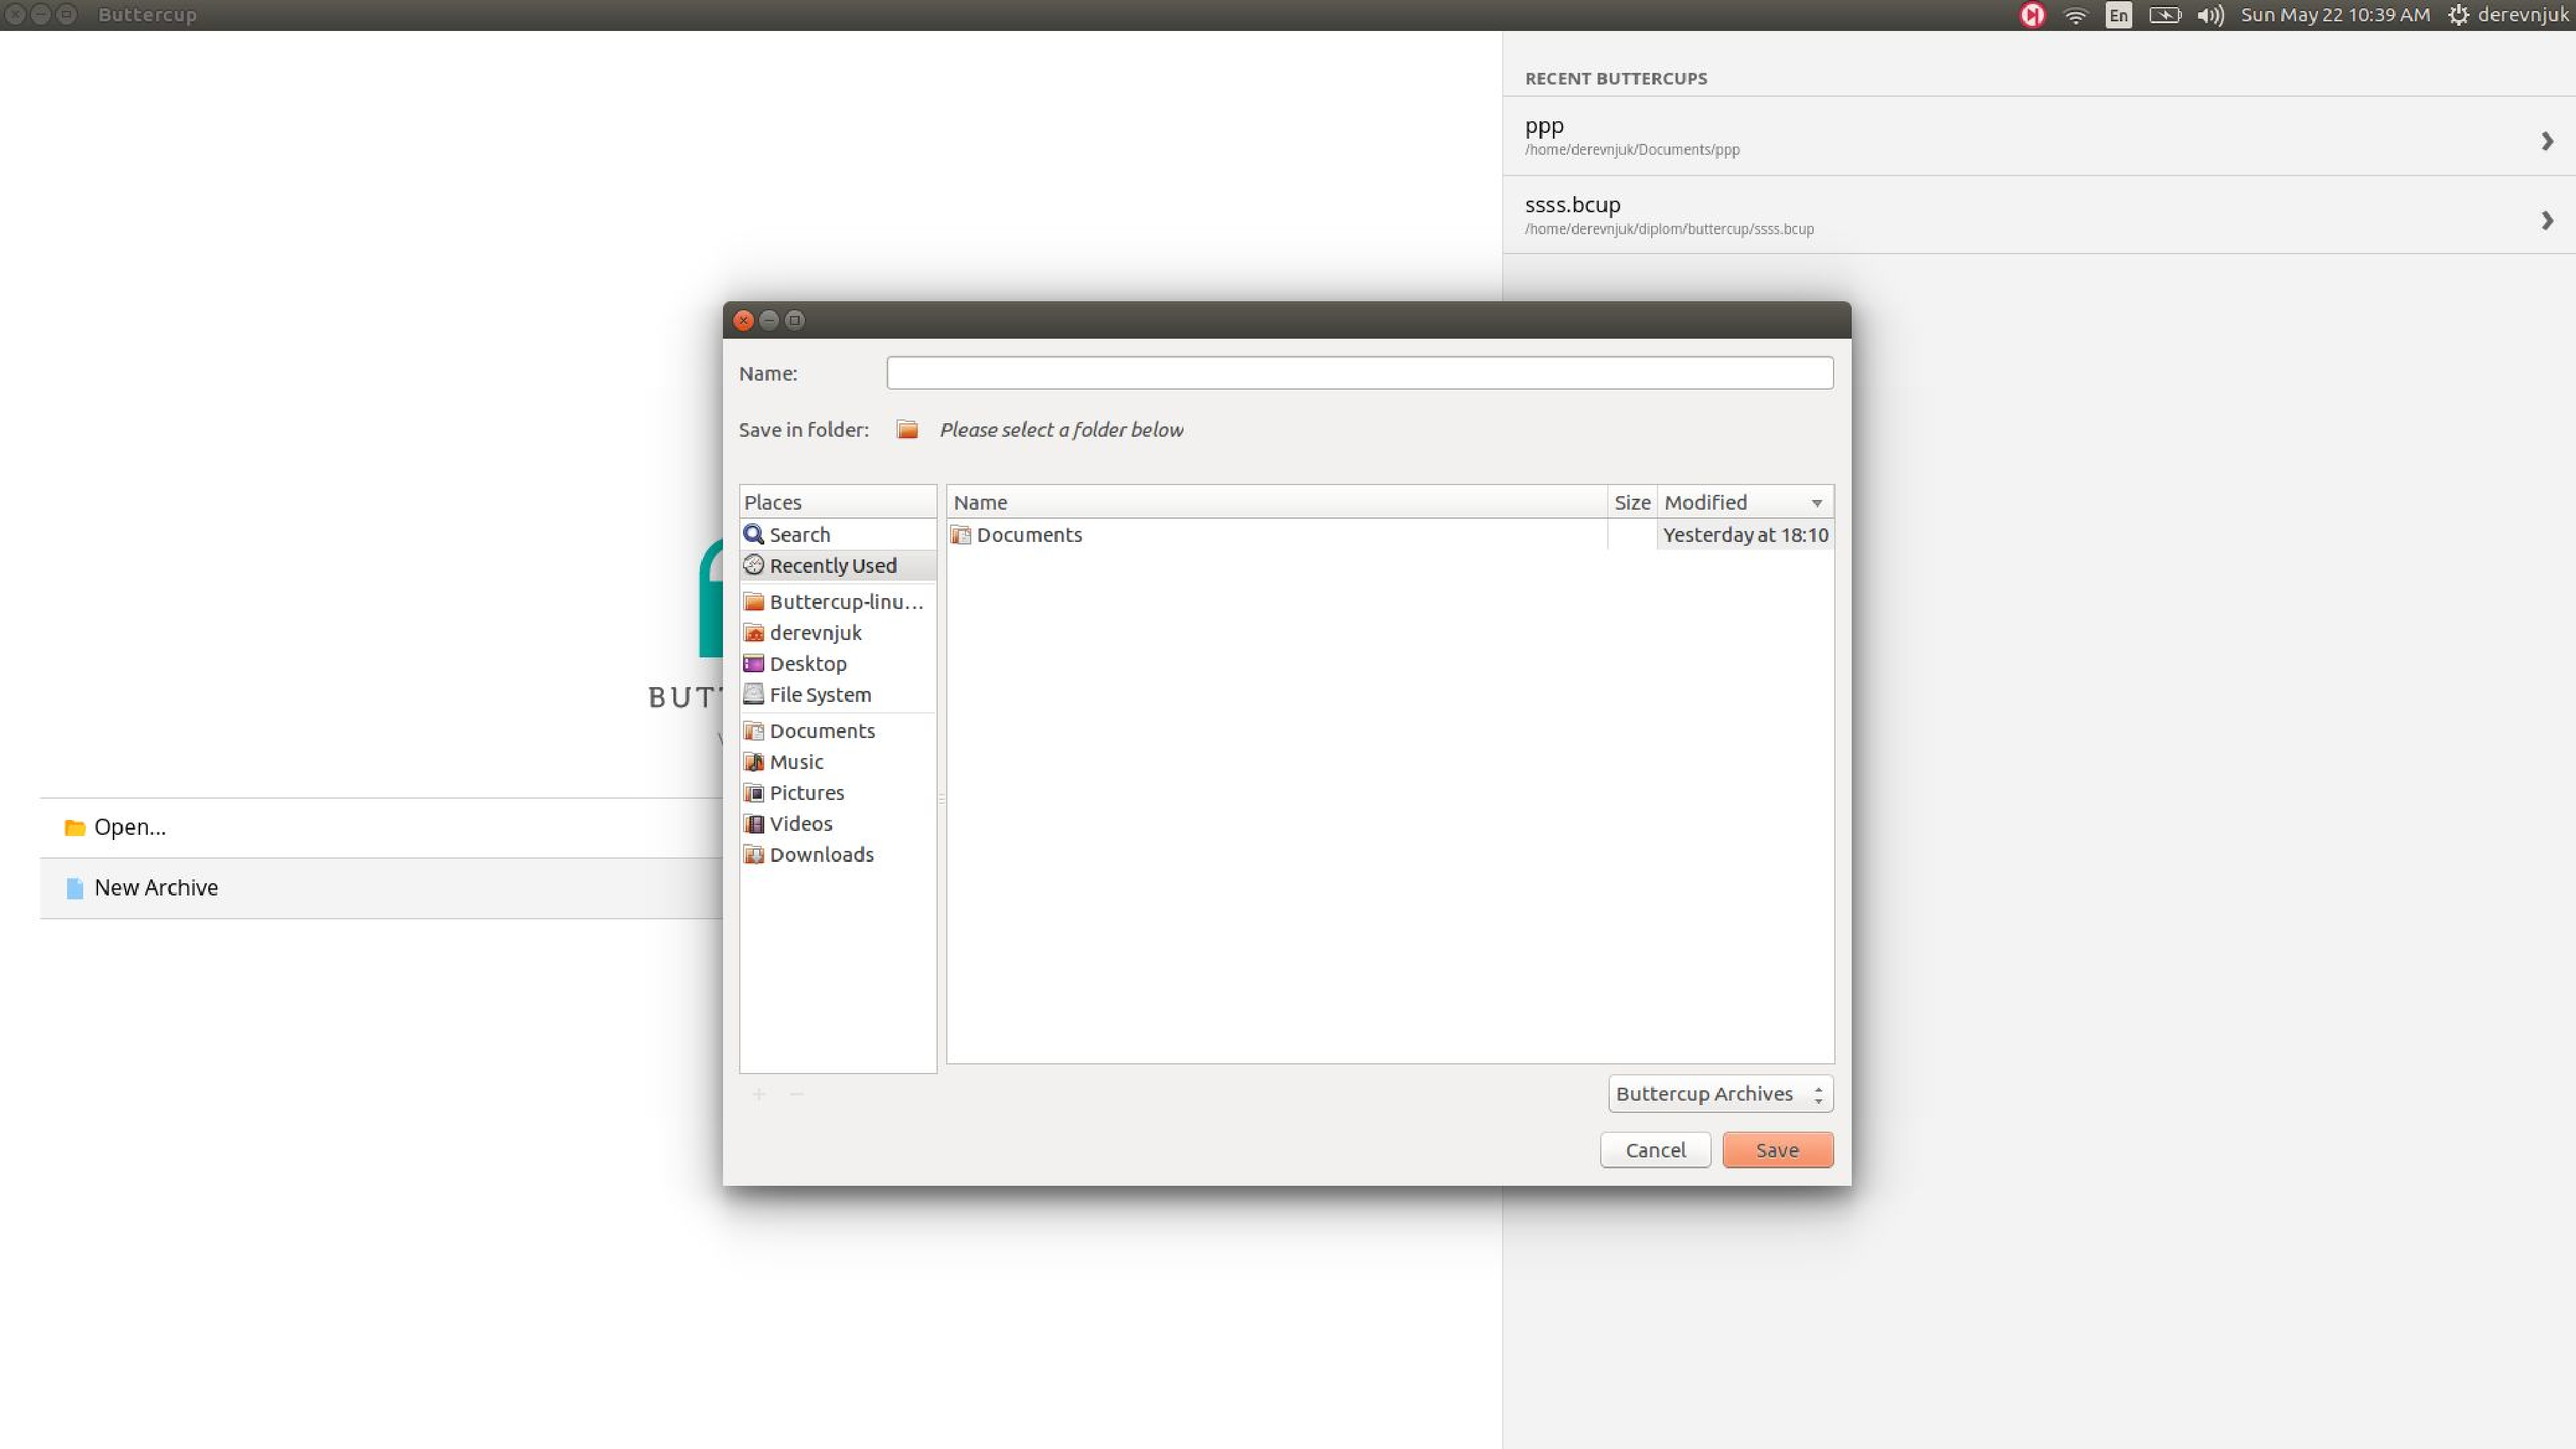
\includegraphics[scale=0.20]{2.pdf}
  \caption{ Окно загрузки/создания хранилища. }
  \label{fig:document:auth:two}
\end{figure}

Пользователь может проверить правильность введенных данных и уйти с формы авторизации через панель активных действий, если передумал. После подтверждения авторизации пользователю предоставляется полный доступ к функционалу системы.

После заполнения полей пользователь переходит ко второму шагу. На нем происходит запрос данных, необходимых для дешифровки и предоставления пользовательских данных. Для входа необходимо ввести один из вариантов логина, пароль доступа и нажать кнопку входа. Также
возможен вход с помощью электронной подписи хранилища. На текущий момент реализован только последних этот подход при аутентификации. Если
пользователь не обладает хранилищем, то следует нажать на кнопку создания хранилища.
После успешного входа откроется главная страница с личными данными пользователя. Представление этого процесса изображено на рисунке~\ref{fig:document:auth:therd}.

\begin{figure}[ht]
\centering
  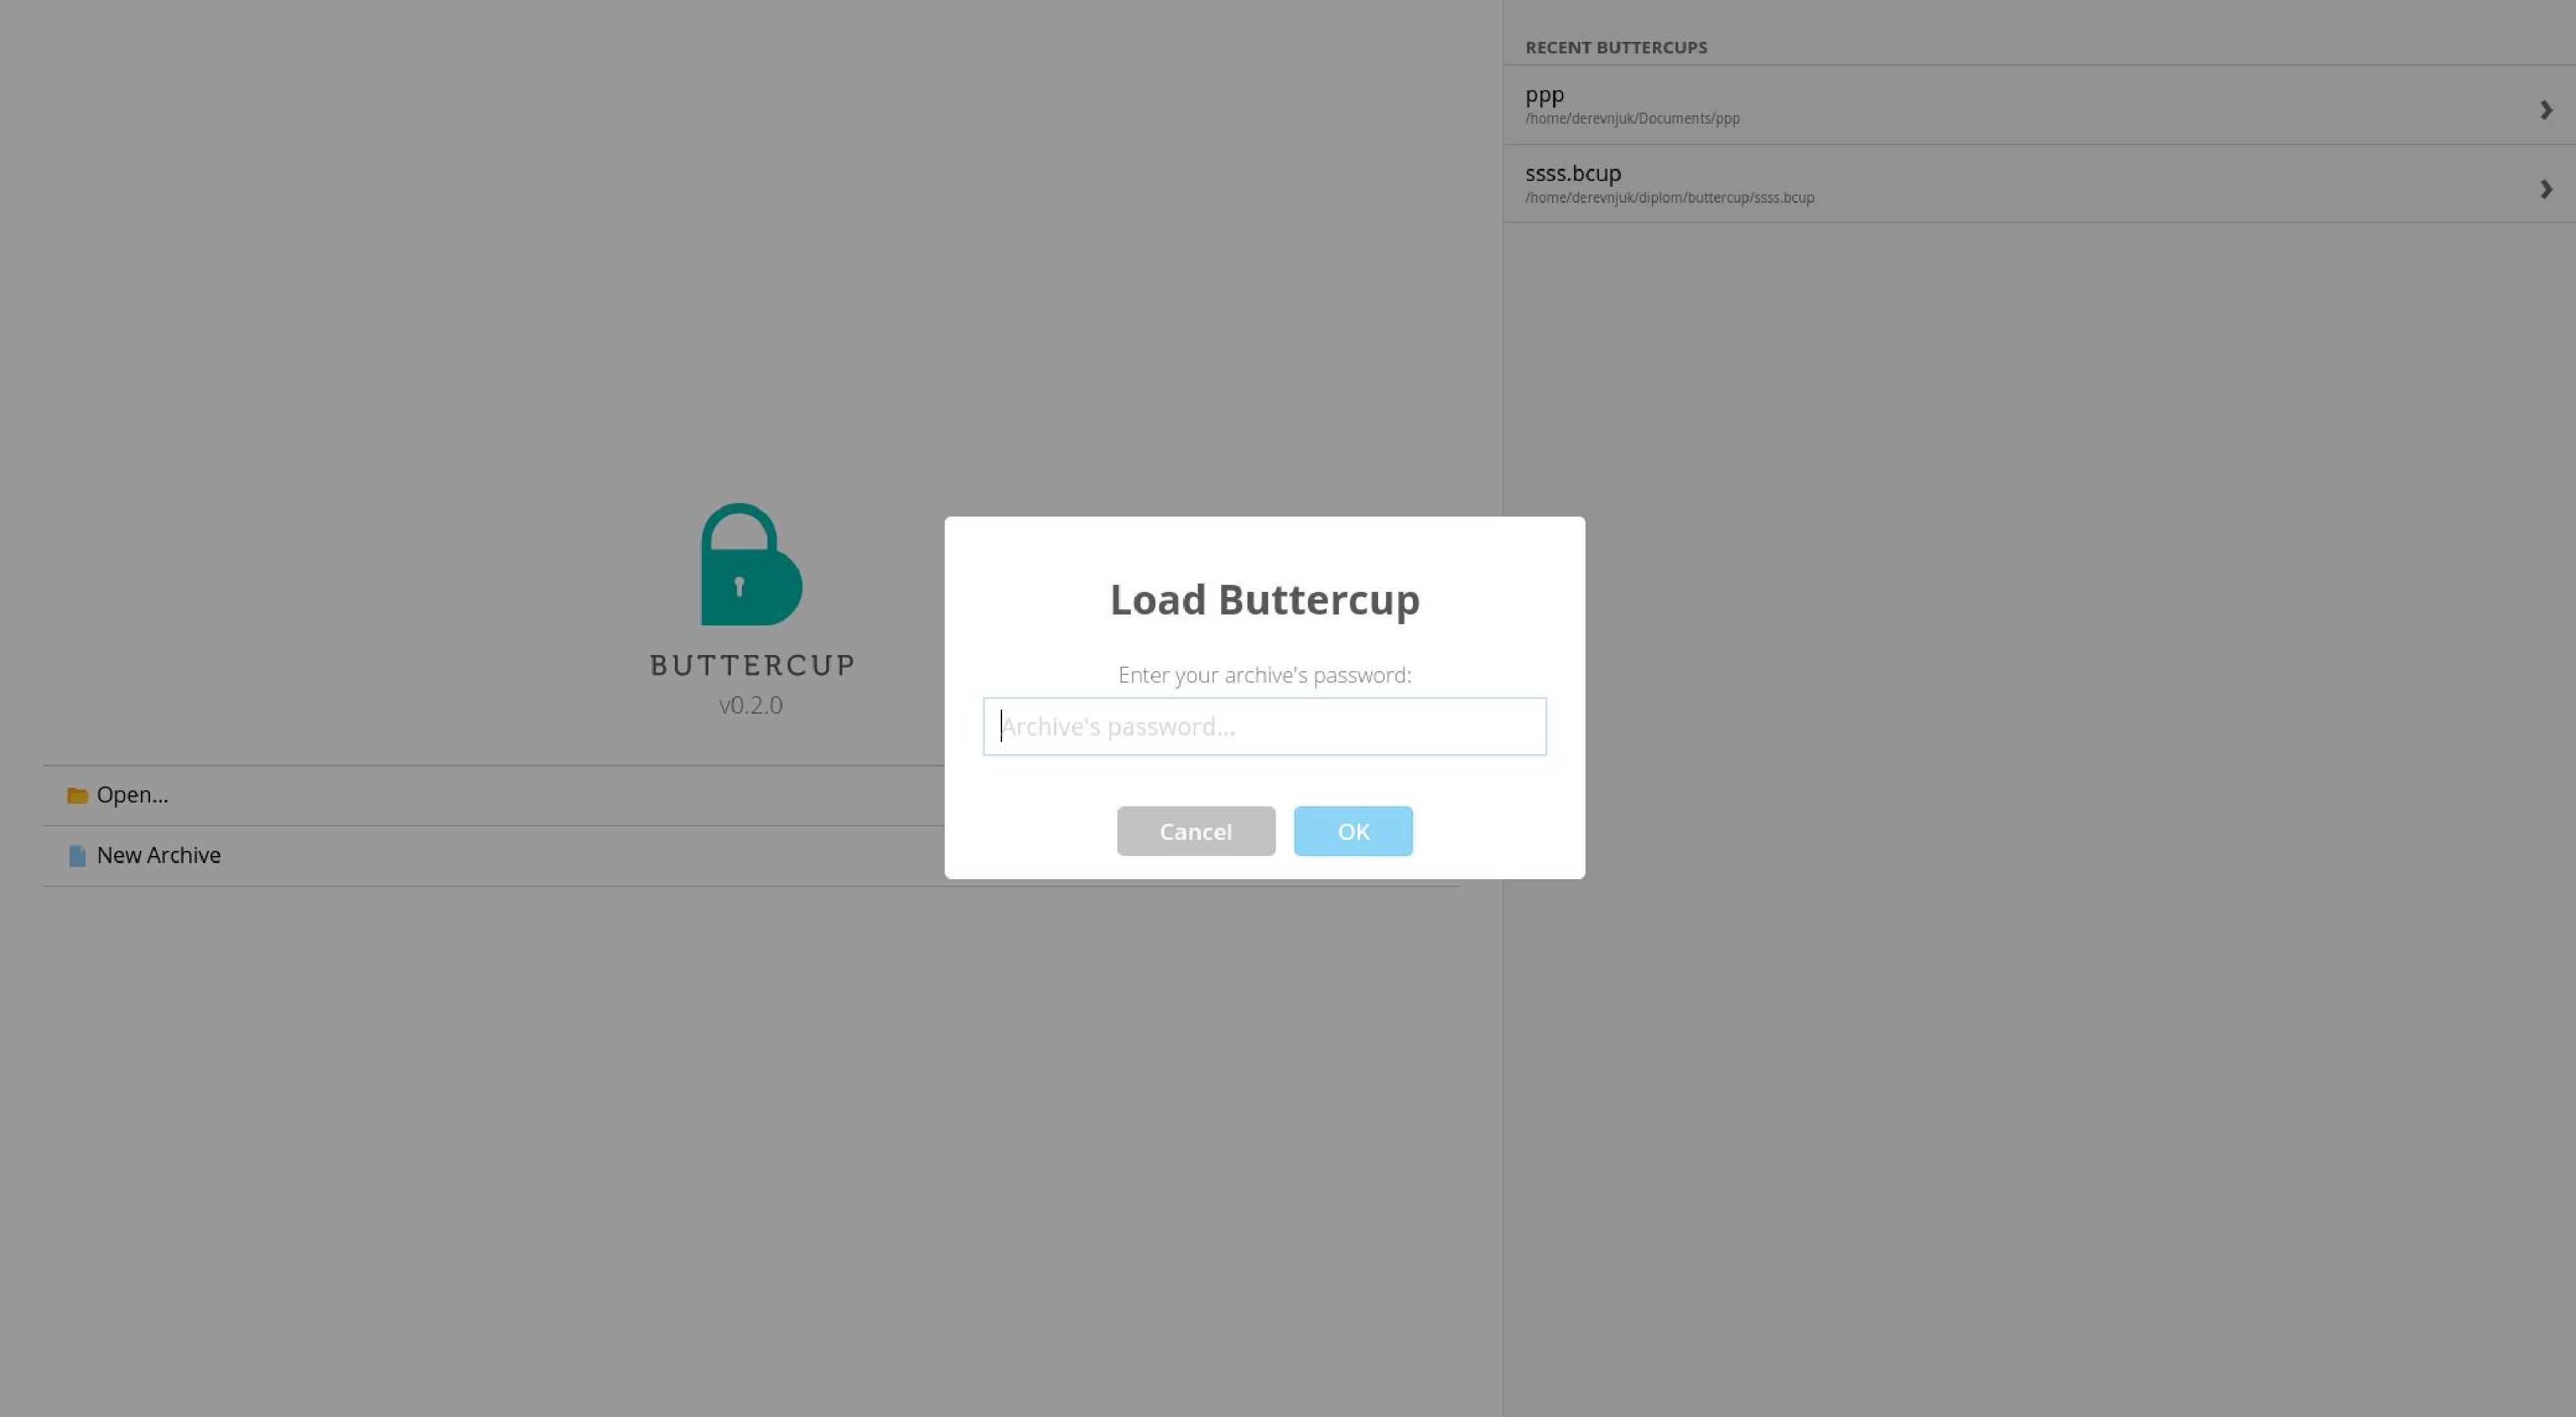
\includegraphics[scale=0.20]{3.pdf}
  \caption{ Окно авторизации пользователя. }
  \label{fig:document:auth:therd}
\end{figure}

При загрузке страницы первым делом производится запрос в базу данных с ключами, которые были переданы в метод контроллера. При некорректных ключах, либо при несуществующей записи в базе, пользователь увидит предупреждающий баннер на красном фоне, который изображен на рисунке~\ref{fig:document:auth:nein}.

\begin{figure}[ht]
\centering
  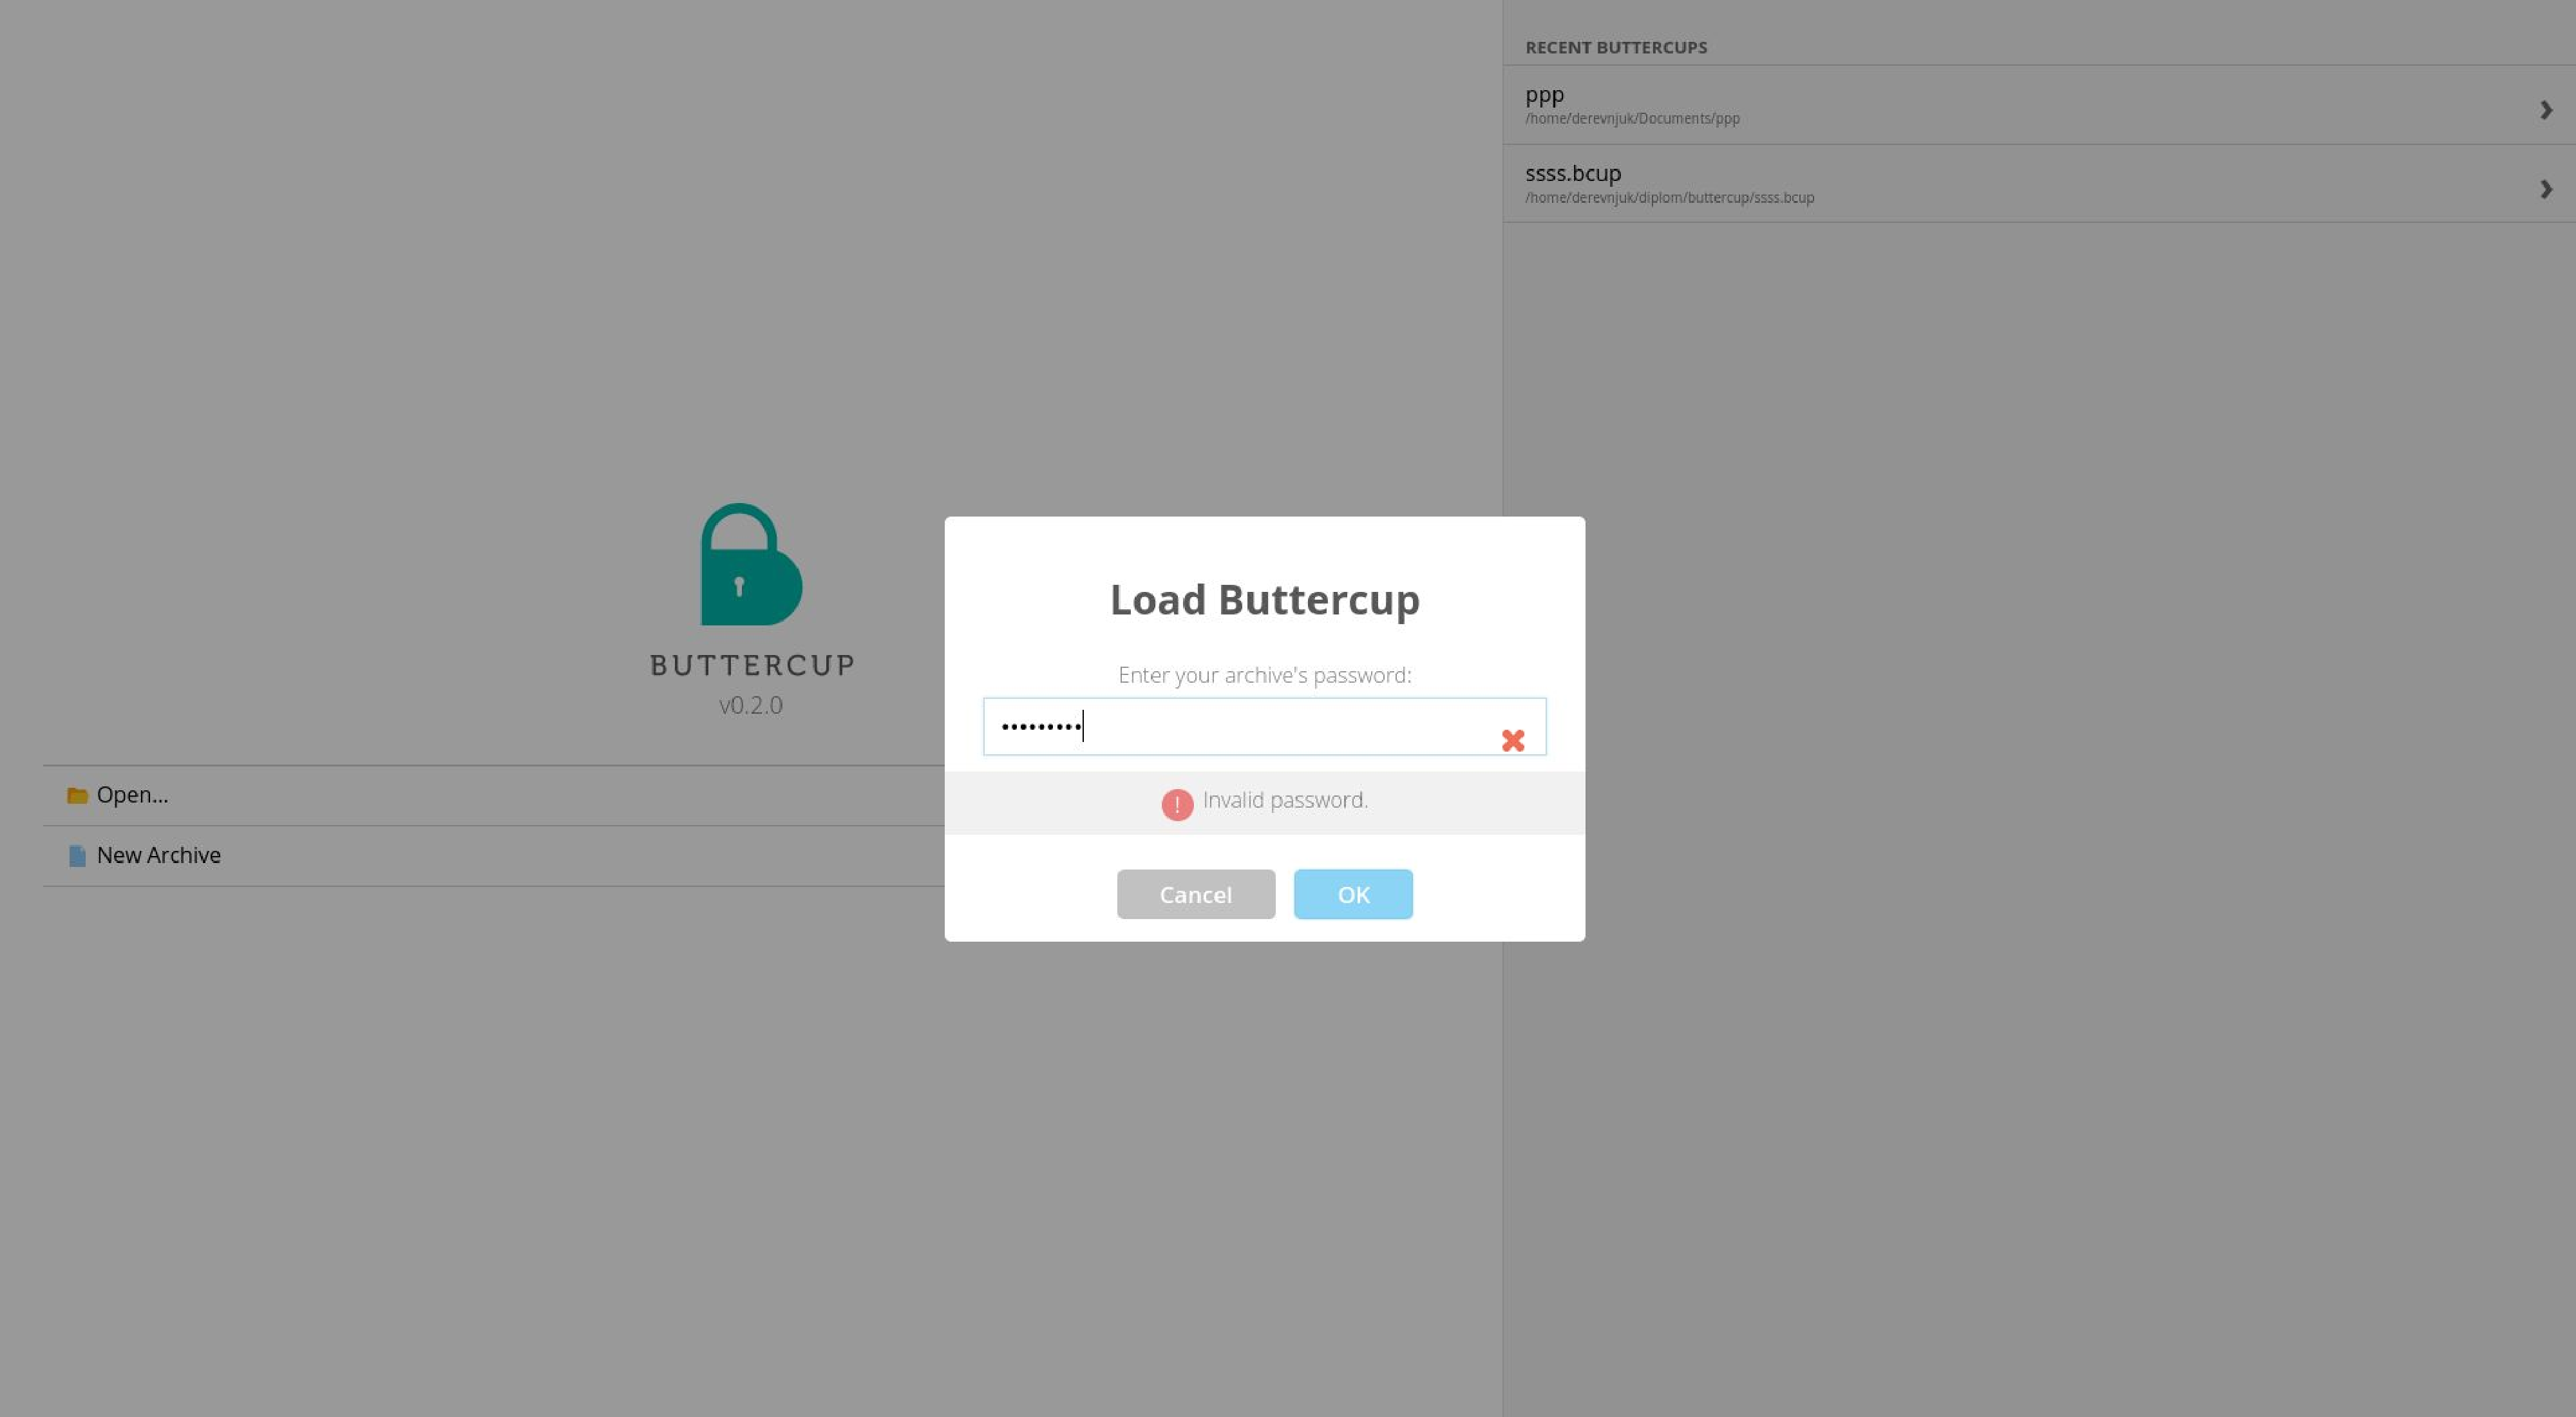
\includegraphics[scale=0.20]{9.pdf}
  \caption{ Окно с неверными ключами. }
  \label{fig:document:auth:nein}
\end{figure}

\subsection{Управление группами в хранилище}
\label{sec:document:created_groupe}

Приложение разработано таким образом, что пользователь не увидит критических сообщений. Все ошибки логируются и сохраняются в базу данных.
Вся работа страницы заключается в управлении и организации составляющих хранилища паролей; в предоставлении доступа к бизнес логике, инкапсулируемой отдельными компонентами.

На основании вышеизложенного, можно выделить шесть основных секций страницы:
\begin{itemize}
	\item дерево группы;
	\item список записей для активной группы;
	\item панель поиска;
	\item область редактора активной записи;
	\item панель активных действий в области групп;
	\item панель активных действий в области записей;
\end{itemize}

Добавление группы в хранилище производится посредством панели активных действий в области групп, которая обращается к собственной валидационной модели. При попытке добавления некорректных данных пользователь получит предупреждение.
Удаление группы в хранилище производится посредством ее собственной панели управления, состоящей из кнопок, предназначенных для удаления и смены ее имени, соотвественно. Процесс удаления группы General, как базовой группы хранилища, представлен на рисунке~\ref{fig:document:created_group:eith}.

\begin{figure}[ht]
\centering
  
\includegraphics[scale=0.20]{8.pdf}
  \caption{ Экран удаление группы. }
  \label{fig:document:created_group:eith}
\end{figure}

\subsection{Управление записями в группе}
\label{sec:document:created_entry}

Добавление в записей производится при помощи панели активных действий в области записей, каждое из которых содержит свою валидационную модель. При попытке добавления некорректных данных пользователь получит предупреждение.

Также пользователь может отредактировать текущий список полей уже сделанной записи, добавив новые или удалив не актуальные. При попытке сохранить или обновить некорректные данные, будет показано сообщение об ошибке. Процесс работы с записью Untitled группы General представлен на рисунке~\ref{fig:document:created_entry:six}:

\begin{figure}[ht]
\centering
  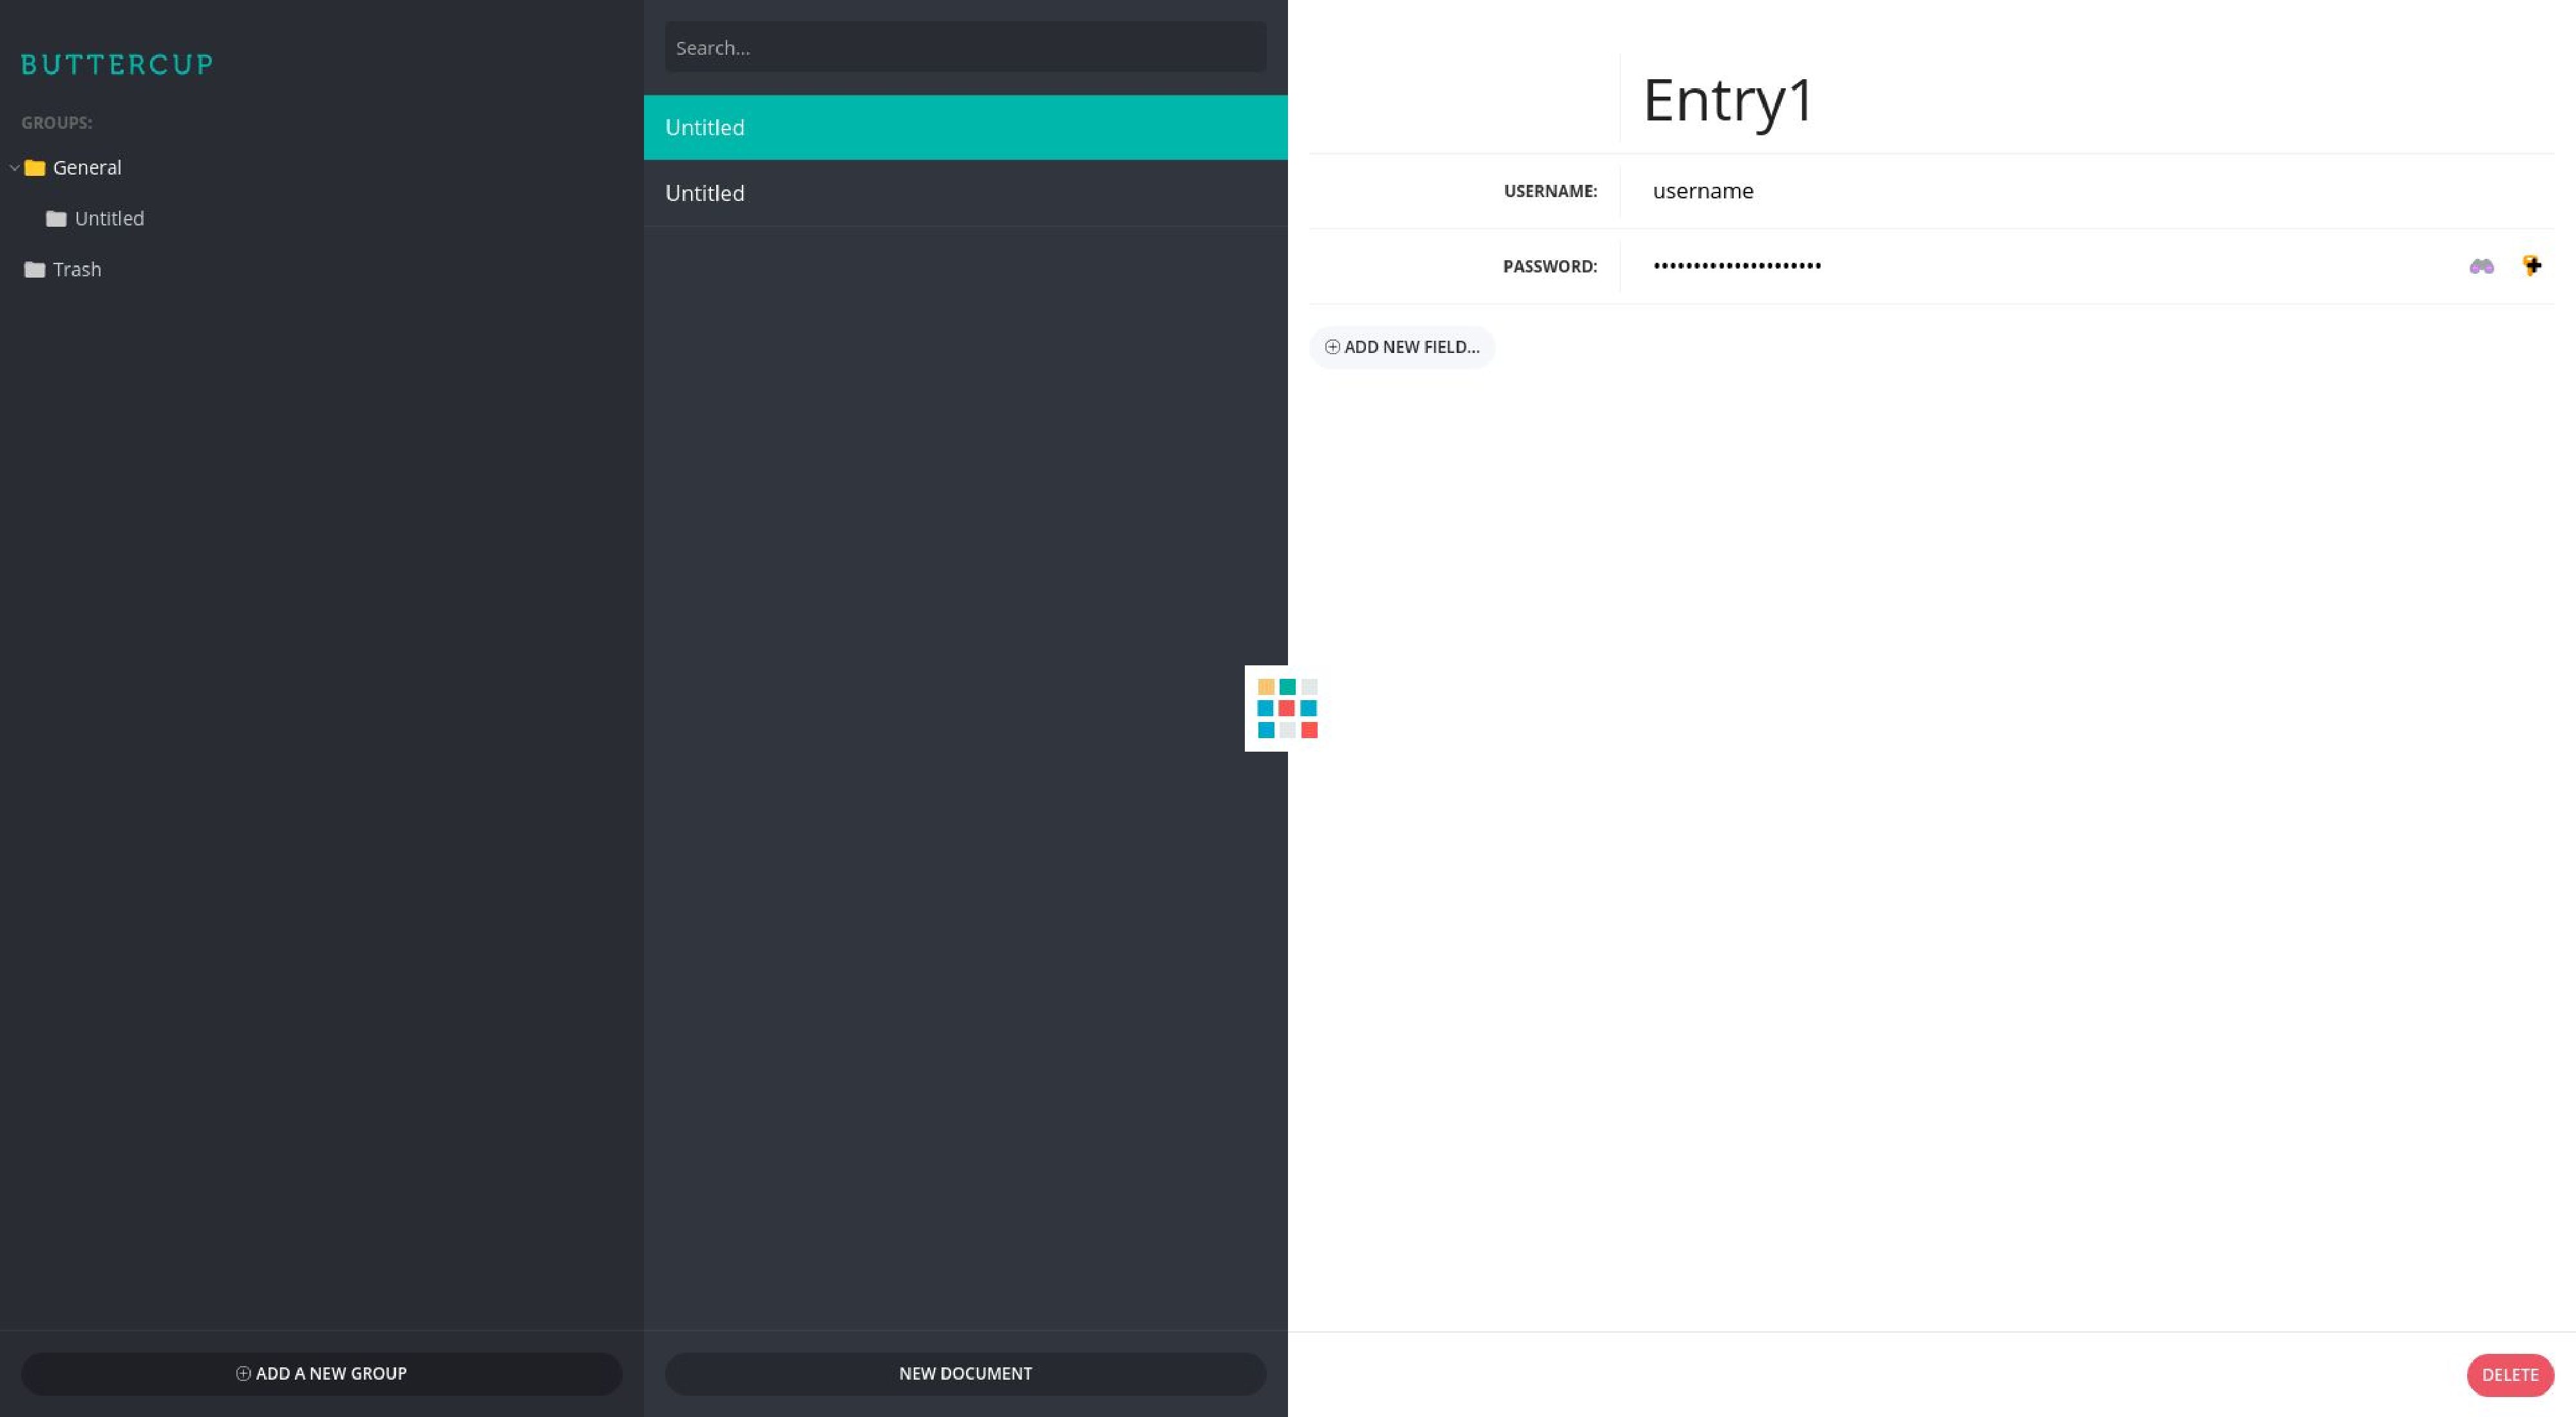
\includegraphics[scale=0.20]{6.pdf}
  \caption{ Экран работы c записью активной группы. }
  \label{fig:document:created_entry:six}
\end{figure}

Удаление записи в группе производится посредством ее собственной панели управления, состоящей из кнопок, предназначенных для удаления и смены ее имени, соотвественно. Процесс удаления записи Untitled группы General, представлен на рисунке~\ref{fig:document:created_entry:seven}.

\begin{figure}[ht]
\centering
  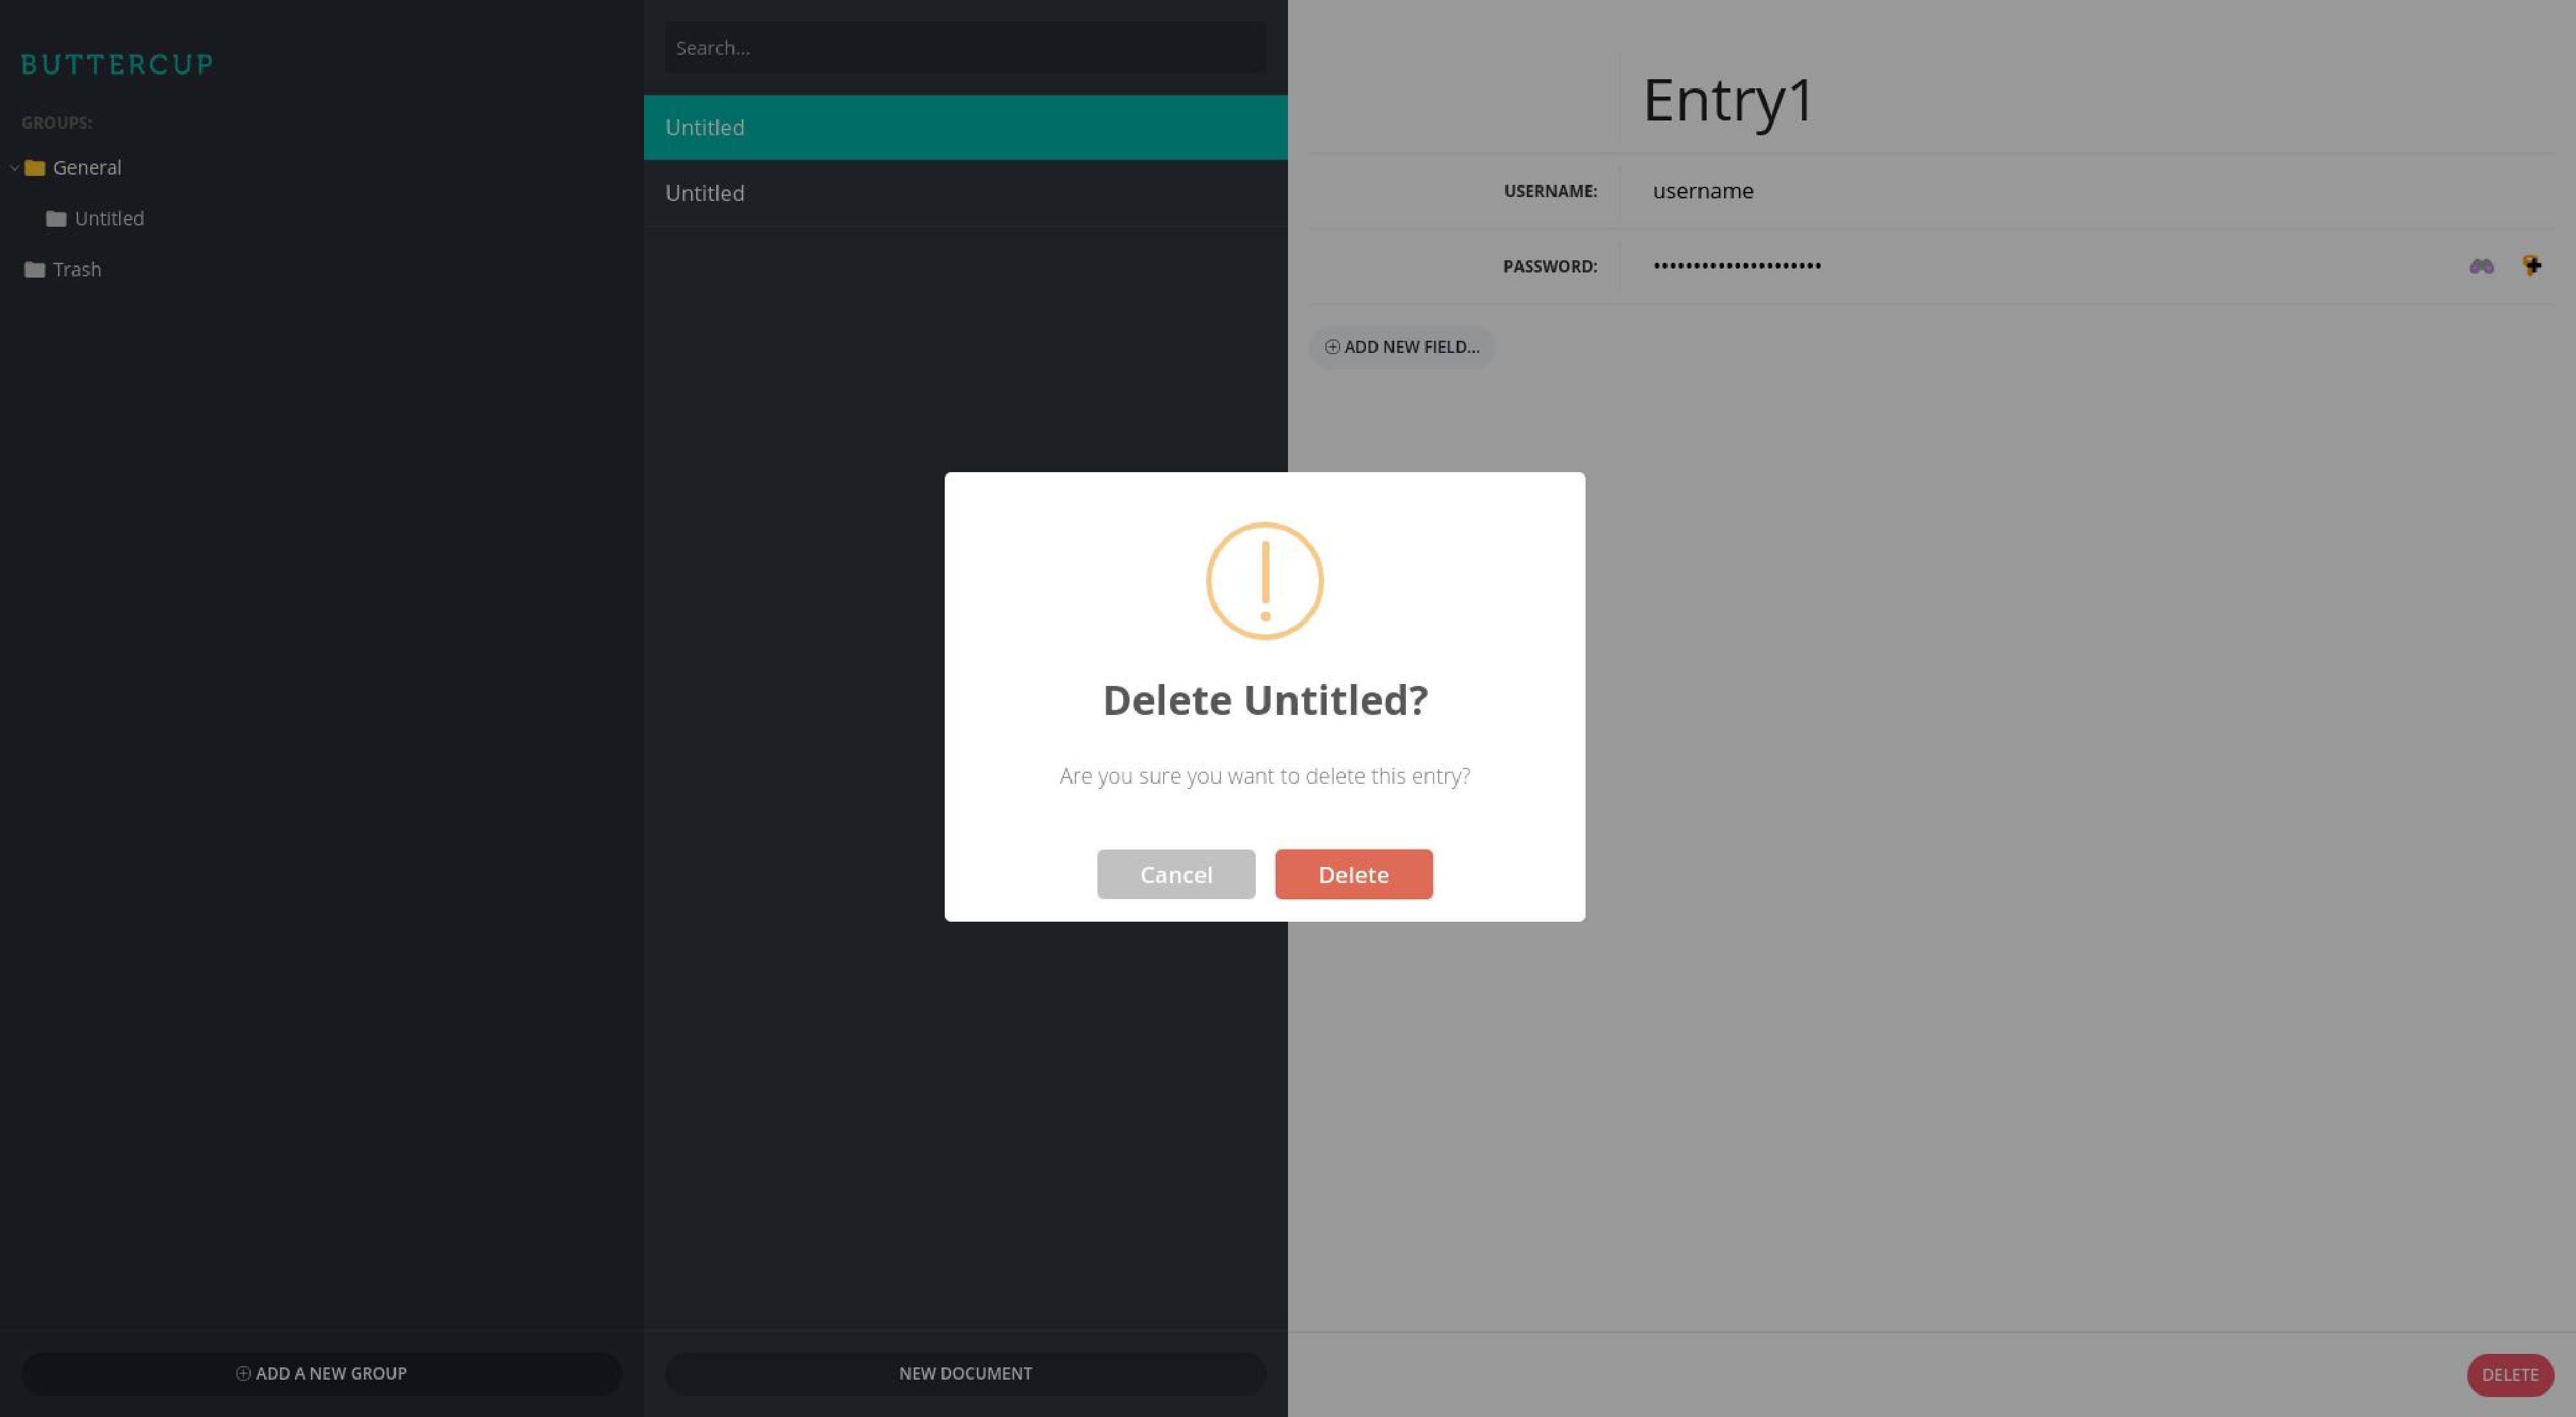
\includegraphics[scale=0.20]{7.pdf}
  \caption{ Экран удаление записи активной группы. }
  \label{fig:document:created_entry:seven}
\end{figure}

\newpage

Поле ввода пароля в области, предназначенной для работы с записью, содержит две иконочные кнопки: первая представляет пароль в читаемом для человека виде, вторая осуществляет генерацию случайного набора символов. В том случае, если была предпринята попытка генерации новой случайной последовательности в качестве пароля, пользователь получит диалоговое окно с предупреждением о вероятности замены текущего пароля, в случае его существования. Экран генерации нового пароля изображен на рисунке~\ref{fig:document:created_entry:ten}.

\begin{figure}[ht]
\centering
  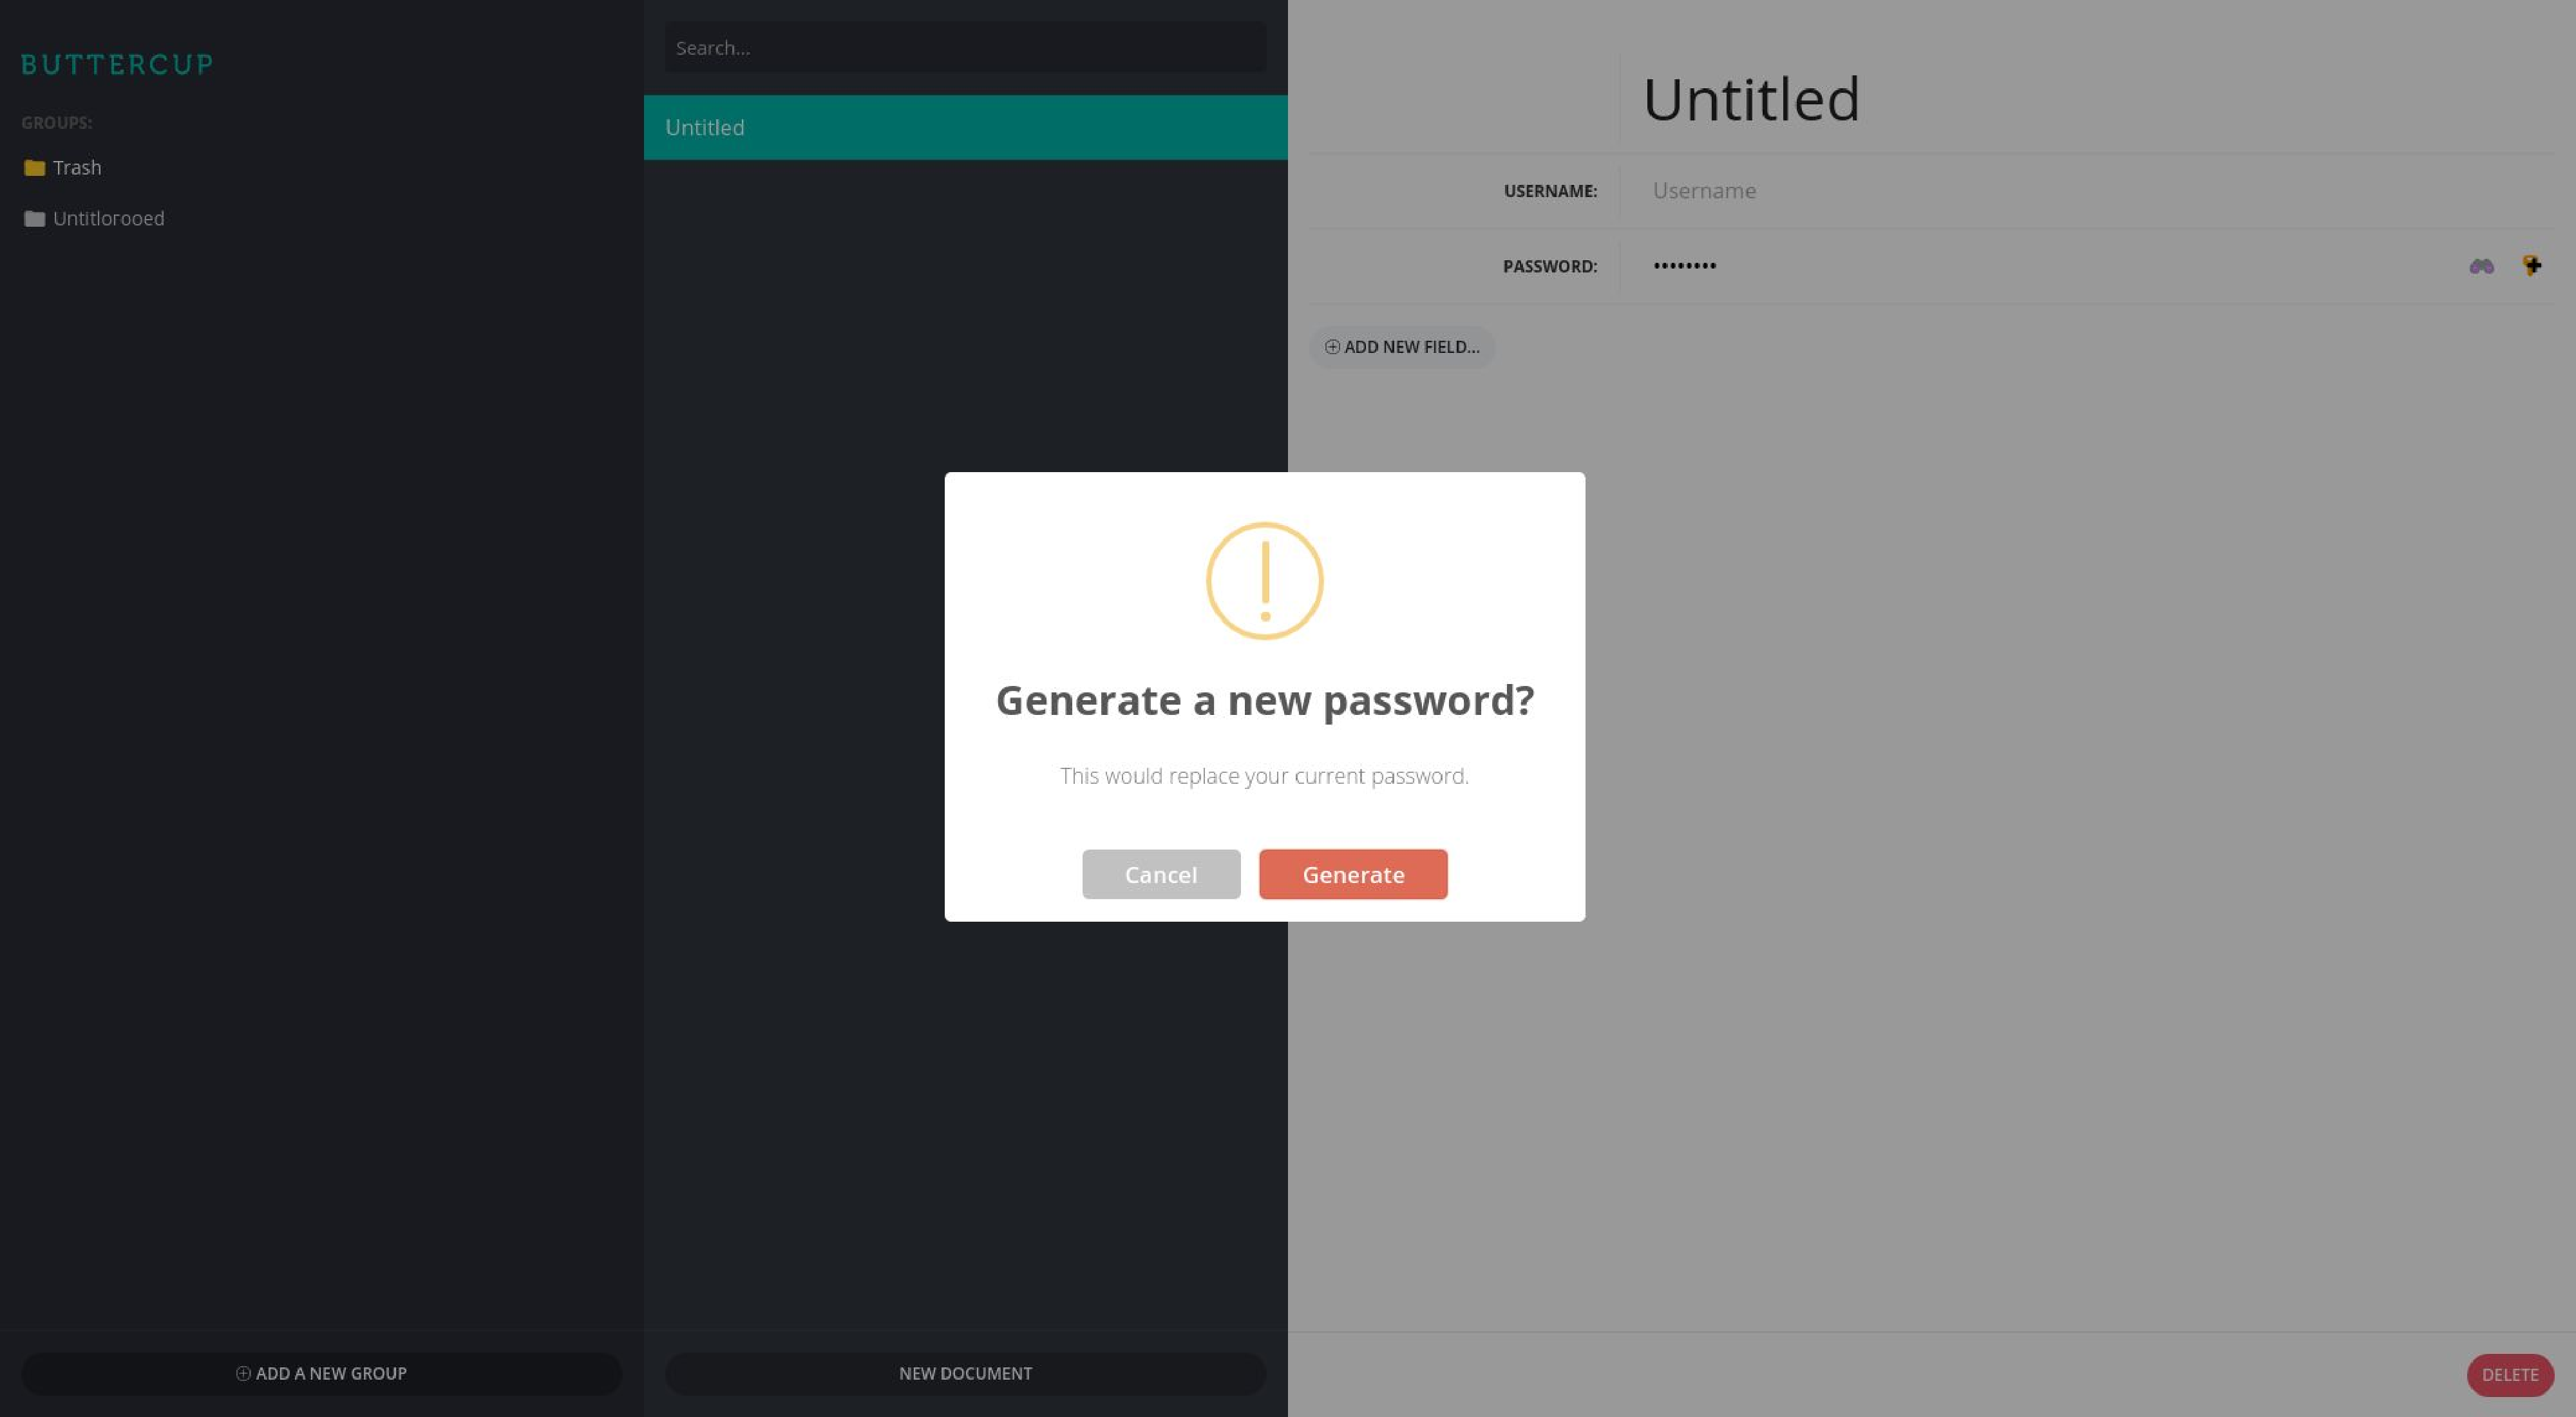
\includegraphics[scale=0.20]{10.pdf}
  \caption{ Экран генерации нового пароля. }
  \label{fig:document:created_entry:ten}
\end{figure}

\newcommand{\byr}{ тыс. бел. руб}

\section{Технико-экономическое обоснование эффективности разработки и использования сетевого менеджера паролей с шифрованием/дешифрованием данных}
\label{sec:econ}

\subsection{Характеристика программного продукта}
\label{sub:econ:desc}

Большое значение для работодателя в современном мире имеет планирование и управление ресурсами и процессами на целом предприятии.
«Сетевой менеджер паролей с шифрованием/дешифрованием данных» представляет собой систему управления пользовательскими данными, имеющими конфиденциальный характер.

Подобные системы внедряются для того, чтобы объединить все данные и все необходимые функции в одной компьютерной системе, которая будет обслуживать текущие потребности пользователей в защите конфиденциальных данных.

Система ведет единую базу данных по всем записям и их группам, так что доступ к информации становится проще, а главное, пользователь получает возможность получить доступ к ней из-под любой платформы.

Экономическая целесообразность инвестиций в разработку и использование программного продукта осуществляется на основе расчета и оценки следующих показателей:
\begin{itemize}
  \item чистая дисконтированная стоимость $ \text{ЧДД} $;
  \item срок окупаемости инвестиций $ \text{ТОК} $;
  \item рентабельность инвестиций $ \text{Р}_\text{и} $.
\end{itemize}

Разработка проектов программных средств связана со значительными затратами ресурсов (трудовых, материальных, финансовых). В связи с этим создание и реализация каждого проекта программного обеспечения нуждается в соответствующем технико-экономическом обосновании (ТЭО).
Для оценки экономической эффективности инвестиционного проекта по разработке и внедрению программного продукта необходимо рассчитать:
\begin{itemize}
  \item результат $ \text{Р} $, получаемый от использования программного продукта;
  \item затраты (инвестиции), необходимые для разработки программного продукта;
  \item показатели эффективности инвестиционного проекта по производству приложения «Сетевой менеджер паролей с шифрованием/дешифрованием данных».
\end{itemize}

\subsection{Расчет стоимостной оценки затрат}
\label{sub:econ:calc_total}

Общие капитальные вложения $ \text{К}_\text{о} $ заказчика (потребителя), связанные с приобретением, внедрением и использованием ПС, рассчитываются по формуле~(\ref{eq:econ:calc_total:totalProgramSize}):
\begin{equation}
  \label{eq:econ:calc_total:totalProgramSize}
  \text{K}_\text{o} = \text{К}_\text{пр} + \text{К}_\text{ос} \text{\,,}
\end{equation}
\begin{explanation}
где & $ \text{К}_\text{пр} $ & затраты пользователя на приобретение ПС по отпускной цене разработчика с учетом стоимости услуг по эксплуатации и сопровождению (тыс. руб.); \\
    & $ \text{К}_\text{ос} $ & затраты пользователя на освоение ПС (тыс. руб.).
\end{explanation}

\subsection{Расчет затрат на разработку и отпускной цены программного продукта}
\label{sub:econ:calc_total_develop}

Основная заработная плата~\cite[с.~59,~приложение 1]{palicyn_2006} исполнителей на разработку приложения «Сетевой менеджер паролей с шифрованием/дешифрованием данных» рассчитывается по формуле~(\ref{eq:econ:calc_total_develop:total_program_size}):
\begin{equation}
  \label{eq:econ:calc_total_develop:total_program_size}
  \text{З}_\text{o} = \sum_{i = 1}^{n}
    \text{Т}_\text{чi} \cdot
    \text{K}\cdot
    \text{Ф}_\text{n}
    \text{\,,}
\end{equation}
\begin{explanation}
где & $ \text{T}_{чi} $ & часовая тарифная ставка i-го исполнителя (тыс. руб.); \\
    & $ \text{Ф}_{n} $ & плановый фонд рабочего времени i-го исполнителя (дн.); \\
    & $ \text{T}_{ч} $ & количество часов работы в день (ч); \\
    & $ \text{K} $ & коэффициент премирования; \\
    & $ n $ & количество исполнителей, занятых разработкой приложения.
\end{explanation}

Коэффициент премирования 1,5. Для расчета заработной платы месячная тарифная ставка 1-го разряда на предприятии установлено на уровне 1850 \byr.
Данные расчетов сведены в таблицу~(\ref{table:econ:calc_total_develop:function_sizes}).

\begin{table}[ht]
\caption{Расчет заработной платы}
\label{table:econ:calc_total_develop:function_sizes}
\centering
  \begin{tabular}{| >{\raggedright}m{0.18\textwidth}
                  | >{\centering}m{0.10\textwidth}
                  | >{\centering}m{0.15\textwidth}
                  | >{\centering}m{0.15\textwidth}
                  | >{\centering}m{0.12\textwidth}
                  | >{\centering\arraybackslash}m{0.14\textwidth}|}
   \hline
   Категория исполнителя & Разряд & Тарифный коэф"=фициент & Часовая тарифная ставка, тыс. руб. & Трудоем"=кость, дн. & Основная заработная плата, тыс. руб. \\
   \hline
   Программист \Rmnum{2}-категории & $ \num{12} $ & $ \num{2,84} $ & $ \num{29,852} $ & $ \num{32} $ & $ \num{11463,273} $\\
   \hline
   Ведущий программист & $ \num{15} $ & $ \num{3,48} $ & $ \num{36,579} $ & $ \num{32} $ & $ \num{14046,546} $ \\
   \hline
   Начальник, руководитель проекта & $ \num{16} $ & $ \num{3,72} $ & $ \num{39,102} $ & $ \num{16} $ & $ \num{7507,636} $\\
   \hline
   Итого с премией (50\%), $ \text{З}_\text{о} $ & $ - $ & $ - $ & $ - $ & $ - $ & $ \num{33017,455} $\\
   \hline
  \end{tabular}
\end{table}

Дополнительная заработная плата на наш программный продукт $ \text{З}_{\text{д}} $, включает выплаты, предусмотренные законодательством о труде (оплата отпусков, льготных часов, времени выполнения государственных обязанностей и других выплат), и определяется по нормативу в процентах к основной заработной плате по формуле~(\ref{eq:econ:calc_total_develop:additional_salary}):
\begin{equation}
  \label{eq:econ:calc_total_develop:additional_salary}
  \text{З}_{\text{д}} =
    \frac {\text{З}_{\text{о}} \cdot \text{Н}_{\text{д}}}
          {100\%} \text{\,,}
\end{equation}
\begin{explanation}
  где & $ \text{Н}_{\text{д}} $ & норматив дополнительной заработной платы, $ \% $.
\end{explanation}

Приняв норматив дополнительной заработной платы $ \text{Н}_{\text{д}} = \num{10\%} $ и подставив известные данные в формулу~(\ref{eq:econ:calc_total_develop:additional_salary}) получим
\begin{equation}
  \label{eq:econ:calc_total_develop:additional_salary_calc}
  \text{З}_{\text{д}} =
    \frac{\num{33017,455} \times 10\%}
         {100\%} \approx \SI{3301,745}{\text{\byr}} \text{\,.}
\end{equation}

Отчисления в фонд социальной защиты населения и обязательное страхование $ \text{З}_{сз} $ определяются в соответствии с действующими законодательными актами по нормативу в процентном отношении к фонду основной и дополнительной зарплаты исполнителей, определенной по нормативу, установленному в целом по организации. Общие отчисления на социальную защиту рассчитываются по формуле~(\ref{eq:econ:calc_total_develop:additional_salary}):
\begin{equation}
  \label{eq:econ:calc_total_develop:soc_prot}
  \text{З}_{\text{сз}} =
    \frac{(\text{З}_{\text{о}} + \text{З}_{\text{д}}) \cdot \text{Н}_{\text{сз}}}
         {\num{100\%}} \text{\,,}
\end{equation}
\begin{explanation}
  где & $ \text{Н}_{\text{сз}} $ & норматив отчислений в фонд социальной защиты населения и на обязательное страхование.
\end{explanation}

Подставив вычисленные ранее значения в формулу~(\ref{eq:econ:calc_total_develop:soc_prot}) получаем:
\begin{equation}
  \label{eq:econ:calc_total_develop:soc_prot_calc}
  \text{З}_{\text{сз}} =
    \frac{ (\num{3017,455} + \num{3301,745}) \times \num{34,6\%} }
         { \num{100\%} }
    \approx \SI{12566,443}{\text{\byr}} \text{\,.}
\end{equation}

Расходы по статье «Машинное время» $ \text{Р}_{м} $ включают оплату машинного времени, необходимого для разработки и отладки программного продукта~\cite[с.\,69, приложениe~6]{palicyn_2006}, которое определяется по нормативам (в машино-часах) на \num{100} строк исходного кода $ \text{H}_{мв} $ машинного времени, и определяются по формуле~(\ref{eq:econ:calc_total_develop:soc_prot}):
\begin{equation}
  \label{eq:econ:calc_total_develop:machine_time}
  \text{Р}_{\text{м}} =
    \text{Ц}_{\text{м}} \cdot
    \text{Т}_{\text{пр}} \text{\,,}
\end{equation}
\begin{explanation}
  где & $ \text{Ц}_{\text{м}} $ & цена одного машино-часа. Рыночная стоимость машино-часа компьютера со всеми необходимым оборудованием, \byr; \\
      & $ \text{T}_{\text{пр}} $ & время работы над программным продуктом, ч.
\end{explanation}

Цена одного часа машинного времени составляет $ \text{Ц}_{\text{м}} = \SI{18}{\text{\byr}} $.
Общее время, затраченное на разработку программного продукта равно \num{252} часа.
Подставляя известные данные в формулу~(\ref{eq:econ:calc_total_develop:machine_time}) получаем:
\begin{equation}
  \label{eq:econ:calc_total_develop:machine_time_calc}
  \text{Р}_{\text{м}} =
    \num{18} \cdot
    \num{252} =
    \SI{4536}{\text{\byr}} \text{\,.}
\end{equation}

Расходы по статье «Научные командировки» $ \text{Р}_{нк} $ на программное средство определяются по формуле~(\ref{eq:econ:calc_total_develop:soc_prot}):
\begin{equation}
  \label{eq:econ:calc_total_develop:business_trip}
  \text{Р}_{\text{нк}} =
    \frac{ \text{З}_{\text{о}} \cdot \text{Н}_{\text{рнк}} }
         { \num{100\%} } \text{\,,}
\end{equation}
\begin{explanation}
  где & $ \text{Н}_{\text{рнк}} $ & норматив расходов на командировки в целом по организации,~$ \% $.
\end{explanation}

Подставляя ранее вычисленные значения в формулу~(\ref{eq:econ:calc_total_develop:business_trip}) и приняв значение $ \text{Н}_{\text{к}} = \num{10\%} $ получаем:
\begin{equation}
  \label{eq:econ:calc_total_develop:business_trip_calc}
    \text{Р}_{\text{нк}} =
    \frac{ \num{33017,455} \times \num{10\%} }
         { \num{100\%} } = \SI{3301,745}{\text{\byr}} \text{\,.}
\end{equation}

Расходы по статье «Прочие затраты» $ \text{П}_{з} $ на программное средство включают затраты на приобретение и подготовку специальной научно-технической информации и специальной литературы. И определяются по формуле~(\ref{eq:econ:calc_total_develop:other_cost}):
\begin{equation}
  \label{eq:econ:calc_total_develop:other_cost}
  \text{П}_{\text{з}} =
    \frac{ \text{З}_{\text{о}} \cdot \text{Н}_{\text{пз}} }
         { \num{100\%} } \text{\,,}
\end{equation}
\begin{explanation}
  где & $ \text{Н}_{\text{пз}} $ & норматив прочих затрат в целом по организации,~$ \% $.
\end{explanation}

Приняв значение норматива прочих затрат $ \text{Н}_{\text{пз}} = \num{20\%} $ и подставив вычисленные ранее значения в формулу~(\ref{eq:econ:calc_total_develop:other_cost}) получаем:
\begin{equation}
  \label{eq:econ:calc_total_develop:other_cost_calc}
  \text{П}_{\text{з}} =
    \frac{ \num{33017,455} \times \num{20\%} }
         { \num{100\%} } =
    \SI{6603,491}{\text{\byr}} \text{\,.}
\end{equation}

Затраты по статье «Накладные расходы» $ \text{Р}_{\text{н}} $, связанные с необходимостью содержания аппарата управления, вспомогательных хозяйств и опытных (экспериментальных) производств, а также с расходами на общехозяйственные нужды $ \text{Р}_{\text{н}} $, и определяют по формуле~(\ref{eq:econ:calc_total_develop:other_cost}):
\begin{equation}
  \label{eq:econ:calc_total_develop:overhead_cost}
  \text{Р}_{\text{н}} =
    \frac{ \text{З}_{\text{о}} \cdot \text{Н}_{\text{рн}} }
         { \num{100\%} } \text{\,,}
\end{equation}
\begin{explanation}
  где & $ \text{Н}_{\text{рн}} $ & норматив накладных расходов в организации,~$ \% $.
\end{explanation}

Приняв норму накладных расходов $ \text{Н}_{\text{рн}} = \num{100\%} $ и подставив известные данные в формулу~(\ref{eq:econ:calc_total_develop:overhead_cost}) получаем:
\begin{equation}
  \label{eq:econ:calc_total_develop:overhead_cost_calc}
  \text{Р}_{\text{н}} =
    \frac{ \num{33017,455} \times \num{100\%} }
         { \num{100\%} } =
    \SI{33017,455}{\text{\byr}} \text{\,.}
\end{equation}

Общая сумма расходов по смете  $ \text{С}_{\text{р}} $ на программный продукт рассчитывается по формуле~(\ref{eq:econ:calc_total_develop:overhead_cost}):
\begin{equation}
  \label{eq:econ:calc_total_develop:overall_cost}
  \text{С}_{\text{р}} =
    \text{З}_{\text{о}} +
    \text{З}_{\text{д}} +
    \text{З}_{\text{сз}} +
    %\text{Н}_{\text{е}} +
    \text{М} +
    % \text{Р}_{\text{с}} + % спецоборудование не нужно
    \text{Р}_{\text{м}} +
    \text{Р}_{\text{нк}} +
    \text{П}_{\text{з}} +
    \text{Р}_{\text{н}}\text{\,.}
\end{equation}

Подставляя ранее вычисленные значения в формулу~(\ref{eq:econ:calc_total_develop:overall_cost}) получаем:
\begin{equation}
  \label{eq:econ:calc_total_develop:overall_cost_calc}
  \text{С}_{\text{р}} = \SI{96344,344}{\text{\byr}} \text{\,.}
\end{equation}

Расходы на сопровождение и адаптацию, которые несет производитель ПО, вычисляются по нормативу от суммы расходов по смете и рассчитываются по формуле~(\ref{eq:econ:calc_total_develop:software_support}):
\begin{equation}
  \label{eq:econ:calc_total_develop:software_support}
  \text{Р}_{\text{са}} =
    \frac { \text{С}_{\text{р}} \cdot \text{Н}_{\text{рса}} }
          { \num{100\%} } \text{\,,}
\end{equation}
\begin{explanation}
  где & $ \text{Н}_{\text{рса}} $ & норматив расходов на сопровождение и адаптацию ПО,~$ \% $.
\end{explanation}

Приняв значение норматива расходов на сопровождение и адаптацию $ \text{Н}_{\text{рса}} = \num{10\%} $ и подставив ранее вычисленные значения в формулу~(\ref{eq:econ:calc_total_develop:software_support}) получаем:
\begin{equation}
  \label{eq:econ:calc_total_develop:software_support_calc}
  \text{Р}_{\text{са}} =
    \frac { \num{96344,334} \times \num{10\%} }
          { \num{100\%} } \approx \SI{9634,433}{\text{\byr}} \text{\,.}
\end{equation}

Общая сумма расходов на разработку (с затратами на сопровождение и адаптацию) как полная себестоимость программно продукта $ \text{С}_{\text{п}} $ определяется по формуле~(\ref{eq:econ:calc_total_develop:base_cost}):
\begin{equation}
  \label{eq:econ:calc_total_develop:base_cost}
  \text{С}_{\text{п}} = \text{С}_{\text{р}} + \text{Р}_{\text{са}} \text{\,.}
\end{equation}

Подставляя известные значения в формулу~(\ref{eq:econ:calc_total_develop:base_cost}) получаем:
\begin{equation}
  \label{eq:econ:calc_total_develop:base_cost_calc}
  \text{С}_{\text{п}} = \num{96344,334} + \num{9634,433} = \SI{105978,768}{\text{\byr}} \text{\,.}
\end{equation}

Разрабатываемое ПО является заказным, т.\,е.~разрабатывается для одного заказчика на заказ.
На основании анализа рыночных условий и договоренности с заказчиком об отпускной цене прогнозируемая рентабельность проекта составит~$ \text{У}_{\text{рп}} = \num{25\%} $.
Прибыль рассчитывается по формуле~(\ref{eq:econ:calc_total_develop:income}):
\begin{equation}
  \label{eq:econ:calc_total_develop:income}
  \text{П}_{\text{о}} =
    \frac { \text{С}_{\text{п}} \cdot \text{У}_{\text{рп}} }
          { \num{100\%} } \text{\,,}
\end{equation}
\begin{explanation}
  где & $ \text{П}_{\text{о}} $ & прибыль от реализации ПО заказчику, \byr; \\
      & $ \text{У}_{\text{рп}} $ & уровень рентабельности ПО,~$ \% $; \\
      & $ \text{C}_{\text{п}} $ & себестоимость программного продукта,~\byr.
\end{explanation}

Подставив известные данные в формулу~(\ref{eq:econ:calc_total_develop:income}) получаем прогнозируемую прибыль от реализации ПО:
\begin{equation}
  \label{eq:econ:income_calc}
  \text{П}_{\text{с}} =
    \frac { \num{105978,768} \times \num{25\%} }
          { \num{100\%} }
    \approx \SI{264694,692}{\text{\byr}} \text{\,.}
\end{equation}

Прогнозируемая цена нашего программного продукта без налогов, вычисляется по формуле~(\ref{eq:econ:calc_total_develop:estimated_price}):
\begin{equation}
  \label{eq:econ:calc_total_develop:estimated_price}
  \text{Ц}_{\text{п}} = \text{С}_{\text{п}} + \text{П}_{\text{о}}  \text{\,.}
\end{equation}

Подставив данные в формулу~(\ref{eq:econ:calc_total_develop:estimated_price}) получаем цену ПО без налогов
\begin{equation}
  \label{eq:econ:calc_total_develop:estimated_price_calc}
  \text{Ц}_{\text{п}} = \num{96344,344}  + \num{26494,692} = \SI{122839,026}{\text{\byr}} \text{\,.}
\end{equation}

\subsection{Расчет стоимостной оценки результата}
\label{sub:econ:calc_price_total}

Результатом $ \text{Р} $ в сфере использования нашего программного продукта является прирост чистой прибыли и амортизационных отчислений~\cite[с.~166\,--\,167]{crundwell_2008}.

\subsubsection{}
\label{sub:econ:calc_price_total:free_money}

Расчет прироста чистой прибыли, которая представляет собой экономию затрат на заработную плату и начислений на заработную плату, полученную в результате внедрения программного продукта, вычисляется по формуле~(\ref{eq:econ:calc_price_total:free_money:free}):
\begin{equation}
  \label{eq:econ:calc_price_total:free_money:free}
  \text{Э}_{\text{з}} =
          { \text{К}_{\text{пр}} \cdot
            \text{(}
            \text{t}_{\text{c}} \cdot
            \text{Т}_{\text{с}} -
            \text{t}_{\text{н}} \cdot
            \text{Т}_{\text{н}}
            \text{)} \cdot
            \text{N}_{\text{n}} \cdot
            \text{(}\num{1} + \frac {\text{H}_{\text{дn}}} {\num{100\%}}\text{)} \cdot
            \text{(}\num{1} + \frac {\text{H}_{\text{нno}}} {\num{100\%}}\text{)}
          } \text{\,,}
\end{equation}
\begin{explanation}
  где & $ \text{N}_{\text{n}} $ & плановый объем работ по анализу и обработки результатов, сколько раз выполнялись в году; \\
      & $ \text{t}_{\text{c}} $ & трудоемкость выполнения работы до внедрения программного продукта, нормо.~ч; \\
      & $ \text{t}_{\text{n}} $ & трудоемкость выполнения работы после внедрения программного продукта, нормо.~ч; \\
      & $ \text{T}_{\text{c}} $ & часовая тарифная ставка, соответствующая разряду выполняемых работ до внедрения программного продукта,~\byr;\\
      & $ \text{T}_{\text{n}} $ & часовая тарифная ставка, соответствующая разряду выполняемых работ после внедрения программного продукта,~\byr; \\
      & $ \text{К}_{\text{пр}} $ & коэффициент премий,~\byr; \\
      & $ \text{Н}_{\text{д}} $ & норматив дополнительной заработной платы,~$ \% $; \\
      & $ \text{Н}_{\text{по}} $ & ставка отчислений в ФСЗН и обязательное страхование,~$ \% $.
\end{explanation}

Приняв значение планового объема работ по анализу и обработки результатов $ \text{N}_{\text{n}} = \num{11} $, трудоемкость выполнения работы до внедрения программного продукта $ \text{t}_{\text{c}} = \num{170} $, трудоемкость выполнения работы после внедрения программного продукта $ \text{t}_{\text{n}} = \num{24} $, часовая тарифная ставка, соответствующая разряду выполняемых работ до внедрения программного продукта $ \text{T}_{\text{c}} = \num{12} $~\byr, часовая тарифная ставка, соответствующая разряду выполняемых работ после внедрения программного продукта $ \text{T}_{\text{n}} = \num{12} $~\byr, коэффициент премий $ \text{К}_{\text{пр}} = \num{1,5} $~\byr, норматив дополнительной заработной платы $ \text{Н}_{\text{д}} = \num{20\%} $, ставку отчислений в ФСЗН и обязательное страхование $ \text{Н}_{\text{по}} = \num{34+0,6\%} $ и подставив ранее вычисленные значения в формулу~(\ref{eq:econ:calc_price_total:free_money:free}) получаем:
\begin{align}
  \label{eq:econ:calc_price_total:free_money:free_calc}
  \text{Э}_{\text{з}} &=
          \num{1,5} \cdot
          \text{(}
          \num{170} \cdot
          \num{12} -
          \num{24} \cdot
          \num{12}
          \text{)} \cdot
          \num{11} \cdot
          \text{(}\num{1} + \frac {\num{20\%}} {\num{100\%}}\text{)} \cdot
          \text{(}\num{1} + \frac {\num{34,6\%}} {\num{100\%}}\text{)} =\notag\\
          &= \SI{42692,201}{\text{\byr}}
          \text{\,.}
\end{align}

Прирост чистой прибыли рассчитывается по формуле~(\ref{eq:econ:calc_price_total:free_money:free_grouw}):
\begin{equation}
  \label{eq:econ:calc_price_total:free_money:free_grouw}
    \text{П}_{\text{ч}} =
    \sum_{i = 1}^{n}
    \text{Э}_\text{i} \cdot
    \text{(}
    \num{1} -
    \frac {\text{H}_{\text{n}}}
    {\num{100\%}}
    \text{)}
    \text{\,,}
\end{equation}
\begin{explanation}
  где & $ \text{n} $ & виды затрат, по которым получена экономия; \\
      & $ \text{Э} $ & сумма экономии, полученная за счет снижения \text{i}-ых затрат,~\byr; \\
      & $ \text{Н}_{\text{n}} $ & ставка налога на прибыль,~$ \% $.
\end{explanation}

Приняв ставку налога на прибыль $ \text{Н}_{\text{n}} = \num{18\%} $ и подставив ранее вычисленные значения в формулу~(\ref{eq:econ:calc_price_total:free_money:free_grouw}) получаем:
\begin{equation}
  \label{eq:econ:calc_price_total:free_money:free_grouw_calc}
  \text{П}_{\text{ч}} =
    \num{42692,201} \cdot
    \text{(}
    \num{1} -
    \frac {\num{18\%}}
    {\num{100\%}}
    \text{)}
    = \SI{34007,605}{\text{\byr}}
    \text{\,.}
\end{equation}

\subsubsection{}
\label{sub:econ:calc_price_total:amort}

Расчет прироста амортизационных отчислений, которые являются источником погашения инвестиций в приобретение программного продукта. Расчет амортизационных отчислений осуществляется по формуле~(\ref{eq:econ:calc_price_total:amort:amort_mf}):
\begin{equation}
  \label{eq:econ:calc_price_total:amort:amort_mf}
    \text{А} =
    \frac {\text{H}_{\text{а}} \cdot \text{И}_{\text{об}}}
    {\num{100\%}}
    \text{\,,}
\end{equation}
\begin{explanation}
  где & $ \text{Н}_{\text{а}} $ & норма амортизации программного продукта,~$ \% $; \\
      & $ \text{И}_{\text{об}} $ & стоимость программного продукта,~\byr.
\end{explanation}

Приняв норму амортизации программного продукта $ \text{Н}_{\text{а}} = \num{20\%} $ и подставив ранее вычисленные значения в формулу~(\ref{eq:econ:calc_price_total:amort:amort_mf}) получаем:
\begin{equation}
  \label{eq:econ:calc_price_total:amort:amort_mf_calc}
  \text{А} =
    \frac {\num{20\%} \cdot \num{122839,026}}
    {\num{100\%}}
    = \SI{24567,805}{\text{\byr}}
    \text{\,.}
\end{equation}

\subsection{Расчет показателей экономической эффективности проекта}
\label{sub:econ:efective}

При оценке эффективности инвестиционных проектов необходимо осуществить приведение затрат и результатов, полученных в разные периоды времени, к  расчетному году,  путем умножения затрат и результатов на коэффициент дисконтирования , который определяется по формуле~(\ref{eq:econ:efective}):
\begin{equation}
  \label{eq:econ:efective:efectiveamort_mf}
    \text{a}_{\text{t}} =
    \frac {\num{1}}
    {\text{(}\num{1} + \text{E}_{\text{н}}\text{)}^{\text{t}-\text{t}_{\text{p}}}}
    \text{\,,}
\end{equation}
\begin{explanation}
  где & $ \text{Е}_{\text{н}} $ & требуемая норма дисконта,~$ \% $; \\
      & $ \text{И}_{\text{об}} $ & порядковый номер года, затраты и результаты которого приводятся к расчетному году; \\
      & $ \text{t}_{\text{p}} $ & расчетный год, в качестве расчетного года принимается год вложения инвестиций, равный \num{1}.
\end{explanation}

Приняв норму дисконта $ \text{Е}_{\text{н}} = \num{25\%} $ и подставив ранее вычисленные значения в формулу~(\ref{eq:econ:efective:efectiveamort_mf}) получаем нормы дисонтирования за четыре года:
\begin{equation}
  \label{eq:econ:efective:efectiveamort_mf_calc}
    \text{a}_{\text{t\num{1}}} =
    \frac {\num{1}}
    {\text{(}\num{1} + \num{0,25}\text{)}^{\num{1}-\num{1}}} = \SI{1}{\text{}}
    \text{\,.}
\end{equation}

\begin{equation}
  \label{eq:econ:efective:efectiveamort_mf_calc}
    \text{a}_{\text{t\num{2}}} =
    \frac {\num{1}}
    {\text{(}\num{1} + \num{0,25}\text{)}^{\num{2}-\num{1}}} = \SI{0,80}{\text{}}
    \text{\,.}
\end{equation}

\begin{equation}
  \label{eq:econ:efective:efectiveamort_mf_calc}
    \text{a}_{\text{t\num{3}}} =
    \frac {\num{1}}
    {\text{(}\num{1} + \num{0,25}\text{)}^{\num{3}-\num{1}}}
    = \SI{0,64}{\text{}}
    \text{\,.}
\end{equation}

\begin{equation}
  \label{eq:econ:efective:efectiveamort_mf_calc}
    \text{a}_{\text{t\num{4}}} =
    \frac {\num{1}}
    {\text{(}\num{1} + \num{0,25}\text{)}^{\num{4}}}
    = \SI{0,51}{\text{}}
    \text{\,.}
\end{equation}

Расчет чистого дисконтированного дохода за четыре года реализации проекта и срока окупаемости инвестиций представлены в таблице~\ref{table:econ:efective:summary}:
\begin{table}[h!]
\caption{Экономические результаты работы предприятия}
\label{table:econ:efective:summary}
\centering
  \begin{tabular}{| >{\raggedright}m{0.205\textwidth}
                  | >{\centering}m{0.09\textwidth}
                  | >{\centering}m{0.06\textwidth}
                  | >{\centering}m{0.115\textwidth}
                  | >{\centering}m{0.115\textwidth}
                  | >{\centering}m{0.115\textwidth}
                  | >{\centering\arraybackslash}m{0.115\textwidth}|}
    \hline
      \multirow{3}{0.20\textwidth}{\centering Показатели} &
      \multirow{3}{0.09\textwidth}{\centering Ед. измер.} &
      \multirow{3}{0.06\textwidth}{\centering Усл. обоз.} &
      \multicolumn{4}{c|}{\centering Значения показателей по шагам} \\

    \cline{4-7}
    & & & & & & \\
    & & & $ t_0 $ & $ t_1 $ & $ t_2 $ & $ t_3 $ \\

    \hline
    Прирост чистой прибыли & \byr & $\Delta\text{П}_{\text{ч}}$ & \num{17503,8} & \num{35007,6} & \num{35007,6} & \num{35007,6} \\

    \hline
    Прирост амортизационных отчислений & \byr & $ \Delta\text{A} $ & \num{24567,8} & \num{24567,8} & \num{24567,8} & \num{24567,8} \\

    \hline
    Прирост результата & \byr & $\Delta\text{Р}_{\text{t}}$ & \num{42071,6} & \num{59575,4} & \num{59575,4} & \num{59575,4} \\

    \hline
    Коэффициент дисконтирования & & $\text{a}_{\text{t}}$ & \num{1} & \num{0,8} & \num{0,64} & \num{0,51} \\

    \hline
    Результат с учетом фактора времени & \byr & $\text{P}_{\text{t}}\text{a}_{\text{t}}$ & \num{42071,6} & \num{47660,3} & \num{38128,3} & \num{33183,5} \\

    \hline
    Инвестиции & \byr & $ \text{И}_{\text{об}} $ & \num{122839,1} & & & \\

    \hline
    Инвестиции с учетом фактора времени & \byr & $\text{И}_{\text{t}}\text{a}_{\text{t}}$ & \num{122839,1} & & & \\

    \hline
    Чистый дисконтированный доход по годам & \byr & $\text{ЧДД}_{\text{t}}$  & \num{-80767,4} & \num{47660,3} & \num{38128,3} & \num{30383,5} \\

    \hline
    ЧДД нарастающим итогом & \byr & $\text{ЧДД} $ & \num{-80767,4} & \num{-33107,1} & \num{5021,2} & \num{35404,6} \\

    \hline

  \end{tabular}
\end{table}

Рассчитаем рентабельность инвестиций $\text{Р}_{\text{и}}$ по формуле~(\ref{eq:econ:efective:renta}):
\begin{equation}
  \label{eq:econ:efective:renta}
    \text{Р}_{\text{и}} =
    \frac {\text{П}_{\text{чср}}}
    {\text{З}} \cdot
    \num{100\%}
    \text{\,,}
\end{equation}
\begin{explanation}
  где & $ \text{З} $ & затраты на приобретения нашего программного продукта,~\byr; \\
      & $ \text{П}_{\text{чср}} $ & среднегодовая величина чистой прибыли за расчетный период, \byr, которая определяется по формуле~(\ref{eq:econ:efective:sumpays}).
\end{explanation}

\begin{equation}
  \label{eq:econ:efective:sumpays}
    \text{П}_{\text{чср}} =
    \frac {\sum_{i = 1}^{n} \cdot \text{П}_\text{чt}}
    {\text{n}}
    \text{\,,}
\end{equation}
\begin{explanation}
  где & $ \text{П}_{\text{чt}} $ & чистая прибыль, полученная в году $\text{t}$,~\byr.
\end{explanation}
\newpage
Подставив данные в формулу~(\ref{eq:econ:efective:sumpays}) получаем среднегодовая величина чистой прибыли:
\begin{align}
  \label{eq:econ:efective:sumpays_calc}
  \text{Ц}_{\text{п}} &=
  \frac {\num{17503,802} + \num{35007,605} + \num{35007,605} + \num{35007,605}}
  {\num{4}} =\notag\\
  &= \SI{30631,654}{\text{\byr}} \text{\,.}
\end{align}

Подставим полученные данные в формулу~(\ref{eq:econ:efective:renta}):
\begin{equation}
  \label{eq:econ:efective:renta_calc}
    \text{Р}_{\text{и}} =
    \frac {\num{30631,654}}
    {\num{122839,026}} \cdot
    \num{100\%}
  = \SI{25}{\text{\%}} \text{\,.}
\end{equation}

В результате технико-экономического обоснования инвестиций по производству нового изделия были получены следующие значения показателей их эффективности:
\begin{itemize}
  \item чистый дисконтированный доход за четыре года производства продукции составит \num{35404,631}~\byr;
  \item треть инвестиций окупаются на четвертый год;
  \item рентабельность инвестиций составляет \num{25\%}.
\end{itemize}

Таким образом, внедрение программного продукта «Сетевой менеджер паролей с шифрованием/дешифрованием данных» для управления и хранения пользовательских данных, является эффективным и инвестиции в его разработку целесообразны с позиции прибыли.

\sectioncentered*{Заключение}
\addcontentsline{toc}{section}{Заключение}

В данном дипломном проекте был рассмотрен процесс разработки сетевого менеджера паролей с шифрованием/дешифрованием данных посредством системы криптографии с открытым ключом.
В рамках дипломного проекта была разработана клиент-серверное приложение для представления и защиты конфиденциальных пользовательских данных.
В разработанном приложении использовались два различных подхода к оценке стойкости генерируемых ключей, на основе принципа функции Эйлера и оценке апостериорной вероятности.
Также для оптимизации вычислительных методов использовались стратегия построения пространства каскадов методов, для решения всех возможных решений.

В результате было получено кроссплатформенное приложение, удовлетворяющее исходным задачам, которые ставились задание на дипломное проектирование.
Результаты работы реализованных в качестве исполняемого модуля в большинстве случаях превосходят по качеству функциональность уже существующего программного обеспечения.
Также был предложен способ улучшения качества поиска простых чисел на малом объеме данных, основанный на предварительной рандомизации экспериментальных данных.
Данный способ удовлетворительно зарекомендовал себя в проведённых тестах.
Помимо предложенной модификации были произведены небольшие улучшения в хорошо известных алгоритмах, направленные на повышение скорости их работы.
Для повышения производительности применялась мемоизация и использовались прологарифмированные версии некоторых методов.

%В итоге получилось раскрыть тему дипломного проекта и создать в его рамках программное обеспечение.
В результате цель дипломного проекта была достигнута.
Было создано программное обеспечение.
Но за рамками рассматриваемой темы осталось еще много других алгоритмов шифрования и интересных вопросов, связанных, например, со статистическим выводом суждений в стойкости синхротронных алгоритмов, нахождением простых чисел для генерации устойчивых ключей и других вопросов, возникающих при работе над приложением.
Эти задачи также являются нетривиальными и требуют детального изучения и проработки.
В дальнейшем планируется развивать и довести существующее программное обеспечение до полноценной сетевого менеджера, способного управлять конфиденциальными данными различной сложности.

\input{references}

\sectioncentered*{Приложение А}
\addcontentsline{toc}{section}{Приложение А (обязательное) Исходный текст класса Archive}

\begin{lstlisting}[style=fsharpstyle,escapeinside={/*@}{@*/}]
(function(module) {

    "use strict";

    var Westley = require("./Westley.js"),
        Inigo = require("./InigoGenerator.js"),
        Flattener = require("./Flattener.js"),
        ManagedGroup = require("./ManagedGroup.js"),
        ManagedEntry = require("./ManagedEntry.js");

    var signing = require("../tools/signing.js"),
        rawSearching = require("../tools/searching-raw.js"),
        instanceSearching = require("../tools/searching-instance.js");

    /**
     * Find entries by searching properties/meta
     * @param {Archive} archive
     * @param {string} check Information to check (property/meta)
     * @param {string} key The key (property/meta-value) to search with
     * @param {RegExp|string} value The value to search for
     * @returns {Array.<ManagedEntry>}
     * @private
     * @static
     * @memberof Archive
     */
    function findEntriesByCheck(archive, check, key, value) {
        return instanceSearching.findEntriesByCheck(
            archive.getGroups(),
            function(entry) {
                var itemValue = (check === "property") ?
                    entry.getProperty(key) || "" :
                    entry.getMeta(key) || "";
                if (value instanceof RegExp) {
                    return value.test(itemValue);
                } else {
                    return itemValue.indexOf(value) >= 0;
                }
            }
        );
    }

    /**
     * The base Buttercup Archive class
     * @class Archive
     */
    var Archive = function() {
        var date = new Date(),
            ts = date.getFullYear() + "-" + (date.getMonth() + 1) + "-" + date.getDate();
        this._westley = new Westley();
        this._getWestley().execute(
            Inigo.create(Inigo.Command.Comment)
                .addArgument('Buttercup archive created (' + ts + ')')
                .generateCommand()
        );
        this._getWestley().execute(
            Inigo.create(Inigo.Command.Format)
                .addArgument(signing.getFormat())
                .generateCommand()
        );
    };

    /**
     * Whether or not this archive has a group with the given title.
     * @param {String} The group's title
     * @returns {true|false}
     * @deprecated Use findGroupsByTitle instead
     * @see findGroupsByTitle
     * @memberof Archive
     */
    Archive.prototype.containsGroupWithTitle = function(groupTitle) {
        return this.findGroupsByTitle(groupTitle).length > 0;
    };

    /**
     * Create a new group
     * @param {string=} title The title for the group
     * @returns {ManagedGroup}
     * @memberof Archive
     */
    Archive.prototype.createGroup = function(title) {
        var managedGroup = ManagedGroup.createNew(this);
        if (title) {
            managedGroup.setTitle(title);
        }
        return managedGroup;
    };

    /**
     * Find entries that match a certain meta property
     * @param {string} metaName The meta property to search for
     * @param {RegExp|string} value The value to search for
     * @returns {Array.<ManagedEntry>}
     * @memberof Archive
     */
    Archive.prototype.findEntriesByMeta = function(metaName, value) {
        return findEntriesByCheck(this, "meta", metaName, value);
    };

    /**
     * Find all entries that match a certain property
     * @param {string} property The property to search with
     * @param {RegExp|string} value The value to search for
     * @returns {Array.<ManagedEntry>}
     * @memberof Archive
     */
    Archive.prototype.findEntriesByProperty = function(property, value) {
        return findEntriesByCheck(this, "property", property, value);
    };

    /**
     * Find all groups within the archive that match a title
     * @param {RegExp|string} title The title to search for, either a string (contained within
     *  a target group's title) or a RegExp to test against the title.
     * @returns {Array.<ManagedGroup>}
     * @memberof Archive
     */
    Archive.prototype.findGroupsByTitle = function(title) {
        return instanceSearching.findGroupsByCheck(
            this.getGroups(),
            function(group) {
                if (title instanceof RegExp) {
                    return title.test(group.getTitle());
                } else {
                    return group.getTitle().indexOf(title) >= 0;
                }
            }
        );
    };

    /**
     * Find an entry by its ID
     * @param {String} The entry's ID
     * @returns {ManagedEntry|null}
     * @memberof Archive
     */
    Archive.prototype.getEntryByID = function(entryID) {
        var westley = this._getWestley();
        var entryRaw = rawSearching.findEntryByID(westley.getDataset().groups, entryID);
        return (entryRaw === null) ? null : new ManagedEntry(this, entryRaw);
    };

    /**
     * Find a group by its ID
     * @param {String} The group's ID
     * @returns {ManagedGroup|null}
     * @memberof Archive
     */
    Archive.prototype.getGroupByID = function(groupID) {
        var westley = this._getWestley();
        var groupRaw = rawSearching.findGroupByID(westley.getDataset().groups, groupID);
        return (groupRaw === null) ? null : new ManagedGroup(this, groupRaw);
    };

    /**
     * Get all groups (root) in the archive
     * @returns {ManagedGroup[]} An array of ManagedGroups
     * @memberof Archive
     */
    Archive.prototype.getGroups = function() {
        var archive = this,
            westley = this._getWestley();
        return (westley.getDataset().groups || []).map(function(rawGroup) {
            return new ManagedGroup(archive, rawGroup);
        });
    };

    /**
     * Get the trash group
     * @returns {ManagedGroup|null}
     * @memberof Archive
     */
    Archive.prototype.getTrashGroup = function() {
        var groups = this.getGroups();
        for (var i = 0, groupsLen = groups.length; i < groupsLen; i += 1) {
            if (groups[i].isTrash()) {
                return groups[i];
            }
        }
        return null;
    };

    /**
     * Perform archive optimisations
     * @memberof Archive
     */
    Archive.prototype.optimise = function() {
        var flattener = new Flattener(this._getWestley());
        if (flattener.canBeFlattened()) {
            flattener.flatten();
        }
    };

    /**
     * Get the underlying Westley instance
     * @protected
     * @returns {Westley}
     * @memberof Archive
     */
    Archive.prototype._getWestley = function() {
        return this._westley;
    };

    /**
     * Create an Archive with the default template
     * @returns {Archive} The new archive
     * @memberof Archive
     * @static
     */
    Archive.createWithDefaults = function() {
        var archive = new Archive(),
            generalGroup = archive.createGroup("General"),
            trashGroup = archive
                .createGroup("Trash")
                    .setAttribute(ManagedGroup.Attributes.Role, "trash");
        return archive;
    };

    module.exports = Archive;

})(module);

\end{lstlisting}

\sectioncentered*{Приложение Б}
\addcontentsline{toc}{section}{Приложение Б (обязательное) Исходный текст класса ManagedGroup}

\begin{lstlisting}[style=fsharpstyle,escapeinside={/*@}{@*/}]
(function(module) {

    "use strict";

    var Inigo = require("./InigoGenerator.js"),
        ManagedEntry = require("./ManagedEntry.js"),
        encoding = require("../tools/encoding.js"),
        searching = require("../tools/searching-raw.js");

    /**
     * Managed group class
     * @class ManagedGroup
     * @param {Archive} archive The archive instance
     * @param {Object} remoteObj The remote object reference
     */
    var ManagedGroup = function(archive, remoteObj) {
        this._archive = archive;
        this._westley = archive._getWestley();
        this._remoteObject = remoteObj;
    };

    /**
     * Create a new entry with a title
     * @param {string=} title
     * @returns {ManagedEntry} The new entry
     * @memberof ManagedGroup
     */
    ManagedGroup.prototype.createEntry = function(title) {
        var managedEntry = ManagedEntry.createNew(this._getArchive(), this.getID());
        if (title) {
            managedEntry.setProperty("title", title);
        }
        return managedEntry;
    };

    /**
     * Create a child group
     * @param {string=} title Optionally set a title
     * @returns {ManagedGroup} The new child group
     * @memberof ManagedGroup
     */
    ManagedGroup.prototype.createGroup = function(title) {
        var group = ManagedGroup.createNew(this._getArchive(), this.getID());
        if (title) {
            group.setTitle(title);
        }
        return group;
    };

    /**
     * Delete the group
     * @memberof ManagedGroup
     */
    ManagedGroup.prototype.delete = function() {
        if (this.isTrash()) {
            throw new Error("Trash group cannot be deleted");
        }
        this._getWestley().execute(
            Inigo.create(Inigo.Command.DeleteGroup)
                .addArgument(this.getID())
                .generateCommand()
        );
        this._getWestley().pad();
        delete this._westley;
        delete this._remoteObject;
    };

    /**
     * Delete an attribute
     * @param {string} attr The name of the attribute
     * @returns {ManagedGroup} Returns self
     * @memberof ManagedGroup
     */
    ManagedGroup.prototype.deleteAttribute = function(attr) {
        this._getWestley().execute(
            Inigo.create(Inigo.Command.DeleteGroupAttribute)
                .addArgument(this.getID())
                .addArgument(attr)
                .generateCommand()
        );
        this._getWestley().pad();
        return this;
    };

    /**
     * Get an attribute
     * @param {string} attributeName The name of the attribute
     * @returns {string|undefined} Returns the attribute or undefined if not found
     * @memberof ManagedGroup
     */
    ManagedGroup.prototype.getAttribute = function(attributeName) {
        var raw = this._getRemoteObject();
        return raw.attributes && raw.attributes.hasOwnProperty(attributeName) ?
            raw.attributes[attributeName] : undefined;
    };

    /**
     * Get the entries within the group
     * @returns {Array.<ManagedEntry>}
     * @memberof ManagedGroup
     */
    ManagedGroup.prototype.getEntries = function() {
        var archive = this._getArchive();
        return (this._getRemoteObject().entries || []).map(function(rawEntry) {
            return new ManagedEntry(archive, rawEntry);
        });
    };

    /**
     * Get the groups within the group
     * @returns {Array.<ManagedGroup>}
     * @memberof ManagedGroup
     */
    ManagedGroup.prototype.getGroups = function() {
        var archive = this._getArchive();
        return (this._getRemoteObject().groups || []).map(function(rawGroup) {
            return new ManagedGroup(archive, rawGroup);
        });
    };

    /**
     * Get the group ID
     * @returns {string}
     * @memberof ManagedGroup
     */
    ManagedGroup.prototype.getID = function() {
        return this._getRemoteObject().id;
    };

    /**
     * Get the group title
     * @returns {string}
     * @memberof ManagedGroup
     */
    ManagedGroup.prototype.getTitle = function() {
        return this._getRemoteObject().title || "";
    };

    /**
     * Check if the current group is used for trash
     * @returns {boolean}
     * @memberof ManagedGroup
     */
    ManagedGroup.prototype.isTrash = function() {
        return this.getAttribute(ManagedGroup.Attributes.Role) === "trash";
    };

    /**
     * Move the group into another
     * @param {ManagedGroup} group The target group (new parent)
     * @returns {ManagedGroup} Returns self
     * @memberof ManagedGroup
     */
    ManagedGroup.prototype.moveToGroup = function(group) {
        if (this.isTrash()) {
            throw new Error("Trash group cannot be moved");
        }
        var targetID = group.getID();
        this._getWestley().execute(
            Inigo.create(Inigo.Command.MoveGroup)
                .addArgument(this.getID())
                .addArgument(targetID)
                .generateCommand()
        );
        this._getWestley().pad();
        return this;
    };

    /**
     * Set an attribute
     * @param {string} attributeName The name of the attribute
     * @param {string} value The value to set
     * @returns {ManagedGroup} Returns self
     * @memberof ManagedGroup
     */
    ManagedGroup.prototype.setAttribute = function(attributeName, value) {
        this._getWestley().execute(
            Inigo.create(Inigo.Command.SetGroupAttribute)
                .addArgument(this.getID())
                .addArgument(attributeName)
                .addArgument(value)
                .generateCommand()
        );
        this._getWestley().pad();
        return this;
    };

    /**
     * Set the group title
     * @param {string} title The title of the group
     * @returns {ManagedGroup} Returns self
     */
    ManagedGroup.prototype.setTitle = function(title) {
        this._getWestley().execute(
            Inigo.create(Inigo.Command.SetGroupTitle)
                .addArgument(this.getID())
                .addArgument(title)
                .generateCommand()
        );
        this._getWestley().pad();
        return this;
    };

    /**
     * Export group to object
     * @returns {Object}
     * @memberof ManagedGroup
     */
    ManagedGroup.prototype.toObject = function() {
        // @todo use object cloning
        var attributes = {},
            groupAttributes = this._remoteObject.attributes || {};
        for (var attrKey in groupAttributes) {
            if (groupAttributes.hasOwnProperty(attrKey)) {
                attributes[attrKey] = groupAttributes[attrKey];
            }
        }
        return {
            id: this.getID(),
            title: this.getTitle(),
            attributes: attributes
        };
    };

    ManagedGroup.prototype.toString = function() {
        return JSON.stringify(this.toObject());
    };

    /**
     * Get the archive instance reference
     * @protected
     * @returns {Archive}
     * @memberof ManagedGroup
     */
    ManagedGroup.prototype._getArchive = function() {
        return this._archive;
    };

    /**
     * Get the remotely-managed object (group)
     * @protected
     * @returns {Object}
     * @memberof ManagedGroup
     */
    ManagedGroup.prototype._getRemoteObject = function() {
        return this._remoteObject;
    };

    /**
     * Get the delta managing instance for the archive
     * @protected
     * @returns {Westley}
     * @memberof ManagedGroup
     */
    ManagedGroup.prototype._getWestley = function() {
        return this._westley;
    };

    ManagedGroup.Attributes = Object.freeze({
        Role:        "bc_group_role"
    });

    /**
     * Create a new ManagedGroup with a delta-manager and parent group ID
     * @static
     * @memberof ManagedGroup
     * @param {Archive} archive
     * @param {string=} parentID The parent group ID (default is root)
     * @returns {ManagedGroup} A new group
     */
    ManagedGroup.createNew = function(archive, parentID) {
        parentID = parentID || "0";
        var id = encoding.getUniqueID(),
            westley = archive._getWestley();
        westley.execute(
            Inigo.create(Inigo.Command.CreateGroup)
                .addArgument(parentID)
                .addArgument(id)
                .generateCommand()
        );
        var group = searching.findGroupByID(westley.getDataset().groups, id);
        return new ManagedGroup(archive, group);
    };

    module.exports = ManagedGroup;

})(module);
\end{lstlisting}

\sectioncentered*{Приложение В}
\addcontentsline{toc}{section}{Приложение В (обязательное) Исходный текст класса EventEmittor}

\begin{lstlisting}[style=fsharpstyle,escapeinside={/*@}{@*/}]
import assert = require('assert');
import Q = require('q');

import collectionutil = require('./base/collectionutil');
import dateutil = require('./base/dateutil');
import err_util = require('./base/err_util');
import event_stream = require('./base/event_stream');
import item_merge = require('./item_merge');
import item_store = require('./item_store');
import key_agent = require('./key_agent');
import logging = require('./base/logging');

export class SyncError extends err_util.BaseError {
	constructor(message: string, sourceErr?: Error) {
		super(message, sourceErr);
	}
}

let syncLog = new logging.BasicLogger('sync');
syncLog.level = logging.Level.Warn;

const REMOTE_STORE = 'cloud';

/** Returns true if two date/times from Item.updatedAt should
  * be considered equal for the purpose of sync.
  *
  * This function accounts for the fact that the resolution
  * of timestamps varies depending on the store - eg.
  * the Agile Keychain format uses timestamps with only
  * second-level resolution whereas local_store.Store supports
  * millisecond-resolution timestamps.
  */
export function itemUpdateTimesEqual(a: Date, b: Date) {
	return dateutil.unixTimestampFromDate(a) ==
	       dateutil.unixTimestampFromDate(b);
}

export enum SyncState {
	/** Sync is not currently in progress */
	Idle,

	/** Sync is enumerating changed items */
	ListingItems,

	/** Sync is fetching and updating changed items */
	SyncingItems
}

export interface SyncProgress {
	state: SyncState;

	/** Count of items that have been synced. */
	updated: number;

	/** Count of items that failed to sync. */
	failed: number;

	/** Total number of changed items to sync. */
	total: number;

	/** Number of items actively being synced. */
	active: number;
}

enum ItemSyncState {
	Unchanged,
	Updated,
	Deleted
}

interface SyncItem {
	localItem: item_store.ItemState;
	localState: ItemSyncState;
	remoteItem: item_store.ItemState;
	remoteState: ItemSyncState;
}

/** Interface for syncing encryption keys and items between
  * a cloud-based store and a local cache.
  */
export interface Syncer {
	onProgress: event_stream.EventStream<SyncProgress>;

	/** Sync encryption keys from the remote store to the local one.
	  * This does not require the remote store to be unlocked.
	  */
	syncKeys(): Q.Promise<void>;

	/** Sync items between the local and remote stores.
	  * Returns a promise which is resolved when the current sync completes.
	  *
	  * Syncing items requires both local and remote stores
	  * to be unlocked first.
	  */
	syncItems(): Q.Promise<SyncProgress>;
}

/** Syncer implementation which syncs changes between an item_store.Store
  * representing a remote store and a local store.
  */
export class EventEmittor implements Syncer {
	private localStore: item_store.SyncableStore;
	private cloudStore: item_store.Store;

	// queue of items left to sync
	private syncQueue: SyncItem[];
	// progress of the current sync
	private syncProgress: SyncProgress;
	// promise for the result of the
	// current sync task or null if no sync
	// is in progress
	private currentSync: Q.Deferred<SyncProgress>;

	onProgress: event_stream.EventStream<SyncProgress>;

	constructor(localStore: item_store.SyncableStore, cloudStore: item_store.Store) {
		this.localStore = localStore;
		this.cloudStore = cloudStore;
		this.onProgress = new event_stream.EventStream<SyncProgress>();
		this.syncQueue = [];
	}

	syncKeys(): Q.Promise<void> {
		let keys = this.cloudStore.listKeys();

		// sync the password hint on a best-effort basis.
		// If no hint is available, display a placeholder instead.
		let hint = this.cloudStore.passwordHint().then(hint => {
			return hint;
		}).catch(err => {
			return '';
		});

		return Q.all([keys, hint]).then((keysAndHint) => {
			var keys = <key_agent.Key[]>keysAndHint[0];
			var hint = <string>keysAndHint[1];
			return this.localStore.saveKeys(keys, hint);
		});
	}

	syncItems(): Q.Promise<SyncProgress> {
		if (this.currentSync) {
			// if a sync is already in progress, complete the current sync first.
			// This should queue up a new sync to complete once the current one finishes.
			return this.currentSync.promise;
		}
		syncLog.info('Starting sync');

		var result = Q.defer<SyncProgress>();
		this.currentSync = result;
		this.currentSync.promise.then(() => {
			syncLog.info('Sync completed');
			this.currentSync = null;
		}).catch(err => {
			syncLog.error('Sync failed', err.toString());
			this.currentSync = null;
		});

		this.syncProgress = {
			state: SyncState.ListingItems,
			active: 0,
			updated: 0,
			failed: 0,
			total: 0
		};

		this.onProgress.listen(() => {
			if (this.syncProgress.state == SyncState.SyncingItems) {
				var processed = this.syncProgress.updated + this.syncProgress.failed;
				syncLog.info({
					updated: this.syncProgress.updated,
					failed: this.syncProgress.failed,
					total: this.syncProgress.total
				});

				if (processed == this.syncProgress.total) {
					this.syncProgress.state = SyncState.Idle;
					this.notifyProgress();
					result.resolve(this.syncProgress);
				} else {
					this.syncNextBatch();
				}
			}
		}, 'sync-progress');
		this.notifyProgress();

		let localItems = this.localStore.listItemStates();
		let remoteItems = this.cloudStore.listItemStates();
		let lastSyncRevisions = this.localStore.lastSyncRevisions(REMOTE_STORE);

		Q.all([localItems, remoteItems, lastSyncRevisions]).then(itemLists => {
			let localItems = <item_store.ItemState[]>itemLists[0];
			let remoteItems = <item_store.ItemState[]>itemLists[1];
			let lastSyncedRevisions = <Map<string, item_store.RevisionPair>>itemLists[2];

			syncLog.info('%d items in local store, %d in remote store', localItems.length, remoteItems.length);

			let allItems: { [index: string]: boolean } = {};

			let localItemMap = collectionutil.listToMap(localItems, item => {
				allItems[item.uuid] = true;
				return item.uuid;
			});
			let remoteItemMap = collectionutil.listToMap(remoteItems, item => {
				allItems[item.uuid] = true;
				return item.uuid;
			});

			Object.keys(allItems).forEach(uuid => {
				let remoteItem = remoteItemMap.get(uuid);
				let localItem = localItemMap.get(uuid);
				let lastSyncedRevision = lastSyncedRevisions.get(uuid);

				this.enqueueItemForSyncIfChanged(localItem, remoteItem, lastSyncedRevision);
			});

			syncLog.info('found %d items to sync', this.syncQueue.length);
			this.syncProgress.state = SyncState.SyncingItems;
			this.notifyProgress();
		}).catch(err => {
			syncLog.error('Failed to list items in local or remote stores', err.stack);
			result.reject(err);

			this.syncProgress.state = SyncState.Idle;
			this.notifyProgress();
		});

		this.syncNextBatch();

		return this.currentSync.promise;
	}

	private enqueueItemForSyncIfChanged(localItem: item_store.ItemState,
		remoteItem: item_store.ItemState,
		lastSyncedRevision?: item_store.RevisionPair) {

		let uuid = localItem ? localItem.uuid : remoteItem.uuid;
		let remoteState = ItemSyncState.Unchanged;
		let localState = ItemSyncState.Unchanged;

		if (localItem) {
			if (localItem.deleted) {
				if (lastSyncedRevision) {
					localState = ItemSyncState.Deleted;
					syncLog.info('item %s deleted locally', uuid);
				}
			} else if (lastSyncedRevision) {
				if (localItem.revision !== lastSyncedRevision.local) {
					localState = ItemSyncState.Updated;
					syncLog.info('item %s updated locally', uuid);
				}
			} else {
				localState = ItemSyncState.Updated;
				syncLog.info('item %s added locally');
			}
		}

		if (remoteItem) {
			if (remoteItem.deleted) {
				if (lastSyncedRevision) {
					remoteState = ItemSyncState.Deleted;
					syncLog.info('item %s deleted in cloud', uuid);
				}
			} else if (lastSyncedRevision) {
				if (remoteItem.revision !== lastSyncedRevision.external) {
					remoteState = ItemSyncState.Updated;
					syncLog.info('item %s updated in cloud', uuid);
				}
			} else {
				remoteState = ItemSyncState.Updated;
				syncLog.info('item %s added in cloud', uuid);
			}
		}

		if (localState !== ItemSyncState.Unchanged ||
			remoteState !== ItemSyncState.Unchanged) {
			this.syncQueue.push({
				localItem: localItem,
				localState: localState,
				remoteItem: remoteItem,
				remoteState: remoteState
			});
			++this.syncProgress.total;
		}
	}

	// sync the next batch of items. This adds items
	// to the queue to sync until the limit of concurrent items
	// being updated at once reaches a limit.
	//
	// When syncing with a store using the Agile Keychain format
	// and Dropbox, there is one file to fetch per-item so this
	// batching nicely maps to network requests that we'll need
	// to make. If we switch to the Cloud Keychain format (or another
	// format) in future which stores multiple items per file,
	// the concept of syncing batches of items may no longer
	// be needed or may need to work differently.
	private syncNextBatch() {
		var SYNC_MAX_ACTIVE_ITEMS = 10;
		while (this.syncProgress.active < SYNC_MAX_ACTIVE_ITEMS &&
			this.syncQueue.length > 0) {
			var next = this.syncQueue.shift();
			this.syncItem(next);
		}
	}

	private notifyProgress() {
		this.onProgress.publish(this.syncProgress);
	}

	// create a tombstone item to represent an item
	// which has been deleted locally or in the cloud during sync
	private createTombstone(store: item_store.Store, uuid: string): item_store.ItemAndContent {
		let item = new item_store.Item(store, uuid);
		item.typeName = item_store.ItemTypes.TOMBSTONE;
		item.updatedAt = new Date();
		return {
			item: item,
			content: null
		};
	}

	private syncItem(item: SyncItem) {
		++this.syncProgress.active;

		var itemDone = (err?: Error) => {
			--this.syncProgress.active;
			if (err) {
				++this.syncProgress.failed;
			} else {
				++this.syncProgress.updated;
			}
			this.notifyProgress();
		};

		// fetch content for local and remote items and the last-synced
		// version of the item in order to perform a 3-way merge
		let uuid = item.localItem ? item.localItem.uuid : item.remoteItem.uuid;
		let localItemContent: Q.Promise<item_store.ItemAndContent>;
		let remoteItemContent: Q.Promise<item_store.ItemAndContent>;

		if (item.localItem) {
			if (item.localItem.deleted) {
				localItemContent = Q(this.createTombstone(this.localStore, uuid));
			} else {
				localItemContent = this.localStore.loadItem(uuid);
			}
		}

		if (item.remoteItem) {
			if (item.remoteItem.deleted) {
				remoteItemContent = Q(this.createTombstone(this.cloudStore, uuid));
			} else {
				remoteItemContent = this.cloudStore.loadItem(uuid);
			}
		}

		let contents = Q.all([localItemContent, remoteItemContent]);
		contents.then((contents: [item_store.ItemAndContent, item_store.ItemAndContent]) => {
			// merge changes between local/remote store items and update the
			// last-synced revision
			let localItem = contents[0];
			let remoteItem = contents[1];
			this.mergeAndSyncItem(localItem, item.localState, remoteItem, item.remoteState)
			.then(() => {
				syncLog.info('Synced changes for item %s', uuid);
				itemDone();
			}).catch((err: Error) => {
				syncLog.error('Syncing item %s failed:', uuid, err);
				var itemErr = new SyncError(`Failed to save updates for item ${uuid}`, err);
				itemDone(itemErr);
			});
		}).catch(err => {
			syncLog.error('Retrieving updates for %s failed:', uuid, err);
			var itemErr = new SyncError(`Failed to retrieve updated item ${uuid}`, err);
			itemDone(itemErr);
		});
	}

	// returns the item and content for the last-synced version of an item,
	// or null if the item has not been synced before
	private getLastSyncedItemRevision(uuid: string): Q.Promise<item_store.ItemAndContent> {
		return this.localStore.getLastSyncedRevision(uuid, REMOTE_STORE).then(revision => {
			if (revision) {
				return this.localStore.loadItem(uuid, revision.local);
			} else {
				return null;
			}
		});
	}

	// given an item from the local and remote stores, one or both of which have changed
	// since the last sync, and the last-synced version of the item, merge
	// changes and save the result to the local/remote store as necessary
	//
	// When the save completes, the last-synced revision is updated in
	// the local store
	private mergeAndSyncItem(localItem: item_store.ItemAndContent,
		localState: ItemSyncState,
		remoteItem: item_store.ItemAndContent,
		remoteState: ItemSyncState) {
		assert(localItem || remoteItem, 'neither local nor remote item specified');

		let remoteRevision: string;
		if (remoteItem && !remoteItem.item.isTombstone()) {
			remoteRevision = remoteItem.item.revision;
			assert(remoteRevision, 'item does not have a remote revision');
		}

		let updatedStoreItem: item_store.Item;
		let saved: Q.Promise<void>;

		// revision of the item which was saved
		let newLocalRevision: string;

		if (localState === ItemSyncState.Updated && remoteState === ItemSyncState.Updated) {
			// item updated both locally and in the cloud, merge changes
			assert(localItem);
			assert(remoteItem);
			syncLog.info('merging local and remote changes for item %s', localItem.item.uuid);

			let mergedStoreItem: item_store.ItemAndContent;
			saved = this.getLastSyncedItemRevision(localItem.item.uuid).then(lastSynced => {
				mergedStoreItem = item_merge.merge(localItem, remoteItem, lastSynced);
				mergedStoreItem.item.updateTimestamps();

				let mergedRemoteItem = item_store.cloneItem(mergedStoreItem, mergedStoreItem.item.uuid);

				return Q.all([
					this.localStore.saveItem(mergedStoreItem.item, item_store.ChangeSource.Sync),
					this.cloudStore.saveItem(mergedRemoteItem.item, item_store.ChangeSource.Sync)
				]);
			}).then(() => {
				assert(mergedStoreItem.item.revision, 'merged local item does not have a revision');
				assert.notEqual(mergedStoreItem.item.revision, localItem.item.revision);

				newLocalRevision = mergedStoreItem.item.revision;
				updatedStoreItem = mergedStoreItem.item;
			});

		} else if (localState !== ItemSyncState.Unchanged) {
			// item added/updated/removed locally
			syncLog.info('syncing item %s from local -> cloud', localItem.item.uuid);
			let clonedItem = item_store.cloneItem(localItem, localItem.item.uuid).item;
			newLocalRevision = localItem.item.revision;
			updatedStoreItem = localItem.item;
			saved = this.cloudStore.saveItem(clonedItem, item_store.ChangeSource.Sync).then(() => {
				remoteRevision = clonedItem.revision;
			});
		} else if (remoteState !== ItemSyncState.Unchanged) {
			// item added/updated/removed in cloud
			syncLog.info('syncing item %s from cloud -> local', remoteItem.item.uuid);
			let clonedItem = item_store.cloneItem(remoteItem, remoteItem.item.uuid).item;
			saved = this.localStore.saveItem(clonedItem, item_store.ChangeSource.Sync).then(() => {
				assert(clonedItem.revision, 'item cloned from remote store does not have a revision');
				newLocalRevision = clonedItem.revision;
				updatedStoreItem = clonedItem;
			});
		}

		return saved.then(() => {
			syncLog.info('setting last synced revisions for %s to %s, %s', updatedStoreItem.uuid, newLocalRevision, remoteRevision);

			let revisions: item_store.RevisionPair;
			if (!updatedStoreItem.isTombstone()) {
				assert(newLocalRevision, 'saved item does not have a revision');
				revisions = { local: newLocalRevision, external: remoteRevision };
			}
			return this.localStore.setLastSyncedRevision(updatedStoreItem, REMOTE_STORE, revisions);
		});
	}
}
\end{lstlisting}

\sectioncentered*{Приложение Г}
\addcontentsline{toc}{section}{Приложение Г (обязательное) Ведомость документов}

% \includepdf позволяет включить в результирующий pdf документ часть другого pdf документа, сделанного
% например не с помощью TeX. Бывает полезно, если какие-то диаграммны нарисованы, например, с помощью
% Microoft Office и сохранены в pdf.
%\includepdf[pages={-}]{documents_list.pdf}

\end{document}